%%%%%%%%%%%%%%%%%%%%%%%%%%%%%%%%%%%%%%%%%%%%%%%%%%%%%%%%%%%%%%%%%%%%%%
%DIF LATEXDIFF DIFFERENCE FILE
%DIF DEL /tmp/claude-0/main_v1_backup.tex   Thu Oct 22 14:30:16 2026
%DIF ADD main.tex                           Thu Oct 22 14:31:49 2026
%DIF 2-4c2-3
%DIF < %% ANTE: Anytime-valid Nonparametric Test of synErgy
%DIF < %% Prepared for Statistics and Computing (Springer) using sn-jnl.
%DIF < %% Reference style: sn-mathphys-ay (Math & Physical Sciences, author-year).
%DIF -------
%% ANTE: Anytime-valid Nonparametric Test of synErgy  (revised version) %DIF > 
%% Springer Nature sn-jnl template, author-year reference style. %DIF > 
%DIF -------
%%%%%%%%%%%%%%%%%%%%%%%%%%%%%%%%%%%%%%%%%%%%%%%%%%%%%%%%%%%%%%%%%%%%%%

\documentclass[pdflatex,sn-mathphys-ay]{sn-jnl}% Math and Physical Sciences Author Year Reference Style

%%%% Standard Packages
\usepackage{graphicx}%
\usepackage{multirow}%
\usepackage{amsmath,amssymb,amsfonts}%
\usepackage{amsthm}%
\usepackage{mathrsfs}%
\usepackage[title]{appendix}%
\usepackage{xcolor}%
\usepackage{textcomp}%
\usepackage{manyfoot}%
\usepackage{booktabs}%
\usepackage{algorithm}%
\usepackage{algorithmicx}%
\usepackage{algpseudocode}%
\usepackage{listings}%

%% Theorem styles
\theoremstyle{thmstyleone}%
\newtheorem{theorem}{Theorem}%
\newtheorem{proposition}[theorem]{Proposition}%
\newtheorem{lemma}[theorem]{Lemma}%
\newtheorem{corollary}[theorem]{Corollary}%

\theoremstyle{thmstyletwo}%
\newtheorem{example}{Example}%
\newtheorem{remark}{Remark}%

\theoremstyle{thmstylethree}%
\newtheorem{definition}{Definition}%
\newtheorem{assumption}{Assumption}%

%% Convenience macros
\newcommand{\E}{\mathbb{E}}
\newcommand{\Prob}{\mathbb{P}}
\newcommand{\Real}{\mathbb{R}}
\newcommand{\F}{\mathcal{F}}
\newcommand{\Syn}{\mathrm{Syn}}
\newcommand{\clip}{\mathrm{clip}}
\newcommand{\indic}{\mathbb{1}}
\DeclareMathOperator*{\argmax}{arg\,max}
\newcommand{\cmk}{\checkmark}
\newcommand{\xmk}{\ensuremath{\times}}

\raggedbottom
%DIF PREAMBLE EXTENSION ADDED BY LATEXDIFF
%DIF UNDERLINE PREAMBLE %DIF PREAMBLE
\RequirePackage[normalem]{ulem} %DIF PREAMBLE
\RequirePackage{color}\definecolor{RED}{rgb}{1,0,0}\definecolor{BLUE}{rgb}{0,0,1} %DIF PREAMBLE
\providecommand{\DIFadd}[1]{{\protect\color{blue}\uwave{#1}}} %DIF PREAMBLE
\providecommand{\DIFdel}[1]{{\protect\color{red}\sout{#1}}}                      %DIF PREAMBLE
%DIF SAFE PREAMBLE %DIF PREAMBLE
\providecommand{\DIFaddbegin}{} %DIF PREAMBLE
\providecommand{\DIFaddend}{} %DIF PREAMBLE
\providecommand{\DIFdelbegin}{} %DIF PREAMBLE
\providecommand{\DIFdelend}{} %DIF PREAMBLE
\providecommand{\DIFmodbegin}{} %DIF PREAMBLE
\providecommand{\DIFmodend}{} %DIF PREAMBLE
%DIF FLOATSAFE PREAMBLE %DIF PREAMBLE
\providecommand{\DIFaddFL}[1]{\DIFadd{#1}} %DIF PREAMBLE
\providecommand{\DIFdelFL}[1]{\DIFdel{#1}} %DIF PREAMBLE
\providecommand{\DIFaddbeginFL}{} %DIF PREAMBLE
\providecommand{\DIFaddendFL}{} %DIF PREAMBLE
\providecommand{\DIFdelbeginFL}{} %DIF PREAMBLE
\providecommand{\DIFdelendFL}{} %DIF PREAMBLE
\newcommand{\DIFscaledelfig}{0.5}
%DIF HIGHLIGHTGRAPHICS PREAMBLE %DIF PREAMBLE
\RequirePackage{settobox} %DIF PREAMBLE
\RequirePackage{letltxmacro} %DIF PREAMBLE
\newsavebox{\DIFdelgraphicsbox} %DIF PREAMBLE
\newlength{\DIFdelgraphicswidth} %DIF PREAMBLE
\newlength{\DIFdelgraphicsheight} %DIF PREAMBLE
% store original definition of \includegraphics %DIF PREAMBLE
\LetLtxMacro{\DIFOincludegraphics}{\includegraphics} %DIF PREAMBLE
\newcommand{\DIFaddincludegraphics}[2][]{{\color{blue}\fbox{\DIFOincludegraphics[#1]{#2}}}} %DIF PREAMBLE
\newcommand{\DIFdelincludegraphics}[2][]{% %DIF PREAMBLE
\sbox{\DIFdelgraphicsbox}{\DIFOincludegraphics[#1]{#2}}% %DIF PREAMBLE
\settoboxwidth{\DIFdelgraphicswidth}{\DIFdelgraphicsbox} %DIF PREAMBLE
\settoboxtotalheight{\DIFdelgraphicsheight}{\DIFdelgraphicsbox} %DIF PREAMBLE
\scalebox{\DIFscaledelfig}{% %DIF PREAMBLE
\parbox[b]{\DIFdelgraphicswidth}{\usebox{\DIFdelgraphicsbox}\\[-\baselineskip] \rule{\DIFdelgraphicswidth}{0em}}\llap{\resizebox{\DIFdelgraphicswidth}{\DIFdelgraphicsheight}{% %DIF PREAMBLE
\setlength{\unitlength}{\DIFdelgraphicswidth}% %DIF PREAMBLE
\begin{picture}(1,1)% %DIF PREAMBLE
\thicklines\linethickness{2pt} %DIF PREAMBLE
{\color[rgb]{1,0,0}\put(0,0){\framebox(1,1){}}}% %DIF PREAMBLE
{\color[rgb]{1,0,0}\put(0,0){\line( 1,1){1}}}% %DIF PREAMBLE
{\color[rgb]{1,0,0}\put(0,1){\line(1,-1){1}}}% %DIF PREAMBLE
\end{picture}% %DIF PREAMBLE
}\hspace*{3pt}}} %DIF PREAMBLE
} %DIF PREAMBLE
\LetLtxMacro{\DIFOaddbegin}{\DIFaddbegin} %DIF PREAMBLE
\LetLtxMacro{\DIFOaddend}{\DIFaddend} %DIF PREAMBLE
\LetLtxMacro{\DIFOdelbegin}{\DIFdelbegin} %DIF PREAMBLE
\LetLtxMacro{\DIFOdelend}{\DIFdelend} %DIF PREAMBLE
\DeclareRobustCommand{\DIFaddbegin}{\DIFOaddbegin \let\includegraphics\DIFaddincludegraphics} %DIF PREAMBLE
\DeclareRobustCommand{\DIFaddend}{\DIFOaddend \let\includegraphics\DIFOincludegraphics} %DIF PREAMBLE
\DeclareRobustCommand{\DIFdelbegin}{\DIFOdelbegin \let\includegraphics\DIFdelincludegraphics} %DIF PREAMBLE
\DeclareRobustCommand{\DIFdelend}{\DIFOaddend \let\includegraphics\DIFOincludegraphics} %DIF PREAMBLE
\LetLtxMacro{\DIFOaddbeginFL}{\DIFaddbeginFL} %DIF PREAMBLE
\LetLtxMacro{\DIFOaddendFL}{\DIFaddendFL} %DIF PREAMBLE
\LetLtxMacro{\DIFOdelbeginFL}{\DIFdelbeginFL} %DIF PREAMBLE
\LetLtxMacro{\DIFOdelendFL}{\DIFdelendFL} %DIF PREAMBLE
\DeclareRobustCommand{\DIFaddbeginFL}{\DIFOaddbeginFL \let\includegraphics\DIFaddincludegraphics} %DIF PREAMBLE
\DeclareRobustCommand{\DIFaddendFL}{\DIFOaddendFL \let\includegraphics\DIFOincludegraphics} %DIF PREAMBLE
\DeclareRobustCommand{\DIFdelbeginFL}{\DIFOdelbeginFL \let\includegraphics\DIFdelincludegraphics} %DIF PREAMBLE
\DeclareRobustCommand{\DIFdelendFL}{\DIFOaddendFL \let\includegraphics\DIFOincludegraphics} %DIF PREAMBLE
%DIF COLORLISTINGS PREAMBLE %DIF PREAMBLE
\RequirePackage{listings} %DIF PREAMBLE
\RequirePackage{color} %DIF PREAMBLE
\lstdefinelanguage{DIFcode}{ %DIF PREAMBLE
%DIF DIFCODE_UNDERLINE %DIF PREAMBLE
  moredelim=[il][\color{red}\sout]{\%DIF\ <\ }, %DIF PREAMBLE
  moredelim=[il][\color{blue}\uwave]{\%DIF\ >\ } %DIF PREAMBLE
} %DIF PREAMBLE
\lstdefinestyle{DIFverbatimstyle}{ %DIF PREAMBLE
	language=DIFcode, %DIF PREAMBLE
	basicstyle=\ttfamily, %DIF PREAMBLE
	columns=fullflexible, %DIF PREAMBLE
	keepspaces=true %DIF PREAMBLE
} %DIF PREAMBLE
\lstnewenvironment{DIFverbatim}{\lstset{style=DIFverbatimstyle}}{} %DIF PREAMBLE
\lstnewenvironment{DIFverbatim*}{\lstset{style=DIFverbatimstyle,showspaces=true}}{} %DIF PREAMBLE
%DIF END PREAMBLE EXTENSION ADDED BY LATEXDIFF

\begin{document}

\DIFdelbegin %DIFDELCMD < \title[Anytime-Valid Testing of Synergistic Causality]{%%%
\DIFdelend \DIFaddbegin \title[Anytime-Valid Sequential Testing of Group Synergy]{\DIFaddend Anytime-Valid \DIFdelbegin \DIFdel{Nonparametric }\DIFdelend \DIFaddbegin \DIFadd{Sequential }\DIFaddend Testing of \DIFdelbegin \DIFdel{Synergistic (}\DIFdelend Group \DIFdelbegin \DIFdel{) Causality}\DIFdelend \DIFaddbegin \DIFadd{Synergy: Interventional and Predictive Formulations}\DIFaddend , with an Application \DIFdelbegin \DIFdel{Establishing Its Absence in Daily }\DIFdelend \DIFaddbegin \DIFadd{to }\DIFaddend Financial Markets}

\author*[1]{\fnm{Quang-Vinh} \sur{Dang}}\email{vinh.dq4@buv.edu.vn}

\affil*[1]{\orgname{British University Vietnam}, \orgaddress{\city{Hung Yen}, \postcode{160000}, \country{Vietnam}}}

\DIFdelbegin %DIFDELCMD < \abstract{Does a \emph{group} of causes act on an effect jointly---beyond the sum
%DIFDELCMD < of its members' separate contributions---and can we decide this \emph{as data
%DIFDELCMD < arrive}, stopping the moment the evidence is conclusive? Every existing test of
%DIFDELCMD < such synergy is fixed-sample: sufficient-cause interaction indices, joint-effect
%DIFDELCMD < estimators, and information-theoretic decompositions (PID, SURD, PEID) all return
%DIFDELCMD < a point value at a pre-committed sample size, with no valid way to monitor
%DIFDELCMD < evidence continuously. We introduce ANTE, an \emph{anytime-valid} nonparametric
%DIFDELCMD < test of a super-additive synergy null built on testing-by-betting. A bounded,
%DIFDELCMD < mean-centred interaction score is accumulated into a nonnegative capital process
%DIFDELCMD < (an e-process); Ville's inequality yields time-uniform Type-I error control under
%DIFDELCMD < optional stopping and continuous monitoring, requiring neither stationarity nor
%DIFDELCMD < correct model specification. We prove validity, a growth (consistency) theorem
%DIFDELCMD < giving power one and an explicit detection-time bound under the alternative, and
%DIFDELCMD < extend the construction to $k$-way groups and to an out-of-sample predictive
%DIFDELCMD < (Granger) synergy for time series. Empirically, ANTE holds its level under
%DIFDELCMD < continuous monitoring where a peeking fixed-sample test inflates tenfold, matches
%DIFDELCMD < the best batch estimators in detection accuracy, and---uniquely---isolates
%DIFDELCMD < genuine interaction from mere joint dependence. Deployed as a demonstrably
%DIFDELCMD < powered instrument, ANTE \emph{establishes} that super-additive group causality
%DIFDELCMD < is \emph{absent} from daily financial markets across thousands of asset triples,
%DIFDELCMD < while it detects the turbulent energy cascade in physics. Synergistic group
%DIFDELCMD < causality is real, but it is not a daily-markets phenomenon.}
%DIFDELCMD < %%%
\DIFdelend \DIFaddbegin \abstract{Does a \emph{group} of variables act on an outcome jointly, beyond the sum
of its members' separate contributions, and can this be decided \emph{as data
arrive}, stopping when the evidence is conclusive? Existing synergy measures
(sufficient-cause interaction indices, joint-effect estimators, information-theoretic
decompositions) are fixed-sample. We introduce ANTE, an anytime-valid sequential test
of a super-additive synergy null built on testing by betting: a bounded interaction score is
accumulated into a nonnegative capital process (an e-process), and Ville's inequality gives
time-uniform Type-I error control under optional stopping. In the \emph{interventional} part
(known randomised design) the null is sequential, $\theta_t\le0$ for all $t$, so stationarity
is not required. In the \emph{predictive} part (ANTE-SG, for time series) the null compares two
learned forecasters, an additive and a joint one, through a truncated-loss score whose bound is
known before each observation; this makes the validity proof exact and replaces a clipping
argument that we show to be invalid in general. We prove validity for the forecaster-comparison
null, power one and a high-probability detection-time bound for an oracle bet, a $k$-way
extension, and bounds on the size of synergy that can be excluded, and we state sufficient
conditions under which a rejection can be read as an $A\times B$ interaction. Simulations show
that the procedure holds its level under continuous monitoring, including heavy-tailed,
correlated and nonstationary nulls, but that its power on real financial noise is low: an injected lagged interaction carrying $40\%$ of the variance of a daily return series is detected in fewer than half of real triples. Type-I control for population-level nulls is checked by simulation and by
placebo calibration on real data, not proved. In a fully specified search of $27{,}027$ hypotheses over financial
panels we find no statistically significant super-additive predictive group effect in daily and
weekly returns and volatility, where the evidence matches a placebo null; for stress indicators and
hourly crypto data the test rejects a true placebo null in $10$--$40\%$ of hypotheses, and we do not interpret
rejections there as synergy.}
\DIFaddend 

\DIFdelbegin %DIFDELCMD < \keywords{anytime-valid inference, e-processes, testing by betting, synergy, group causality, Granger causality}
%DIFDELCMD < %%%
\DIFdelend \DIFaddbegin \keywords{anytime-valid inference, e-processes, testing by betting, synergy, group causality, predictive synergy, Granger causality}
\DIFaddend 

\pacs[MSC Classification]{62L10, 62M10, 62G10, 91G70}

\maketitle

%%==========================================================%%
\section{Introduction}\label{sec:intro}

Some effects require a coalition. Two drugs that are inert alone can be lethal
together; two genes silent in isolation can jointly switch on a phenotype; two
market shocks, each absorbed on its own, can compound into a crisis. The common
structure is \emph{synergy}: the joint action of a set of \DIFdelbegin \DIFdel{causes }\DIFdelend \DIFaddbegin \DIFadd{variables }\DIFaddend exceeds the sum
of their individual actions. \DIFdelbegin \DIFdel{Detecting synergy---distinguishing }\DIFdelend \DIFaddbegin \DIFadd{Distinguishing }\DIFaddend ``you need
\emph{both} $A$ and $B$'' from ``$A$ helps and $B$ helps, separately''
\DIFdelbegin \DIFdel{---is }\DIFdelend \DIFaddbegin \DIFadd{is }\DIFaddend a recurring scientific question, and a \DIFdelbegin \DIFdel{surprisingly }\DIFdelend subtle one, because it is a
statement about an \emph{interaction}, not about any single \DIFdelbegin \DIFdel{cause}\DIFdelend \DIFaddbegin \DIFadd{variable}\DIFaddend .

The question has been formalised at least three times, in \DIFdelbegin \DIFdel{mutually unaware
}\DIFdelend \DIFaddbegin \DIFadd{largely separate
}\DIFaddend literatures. In epidemiology, Rothman's sufficient-component-cause model
\citep{rothman1976} defines synergy as two factors being component causes of the
same causal ``pie'', measured by the additive-scale interaction contrast and its
relative-excess-risk index \citep{hosmer1992,vanderweele2014}, with a complete
counterfactual axiomatisation for arbitrarily many binary causes due to
\citet{vanderweele2012} and, \DIFdelbegin \DIFdel{very }\DIFdelend \DIFaddbegin \DIFadd{more }\DIFaddend recently, a multi-factor generalized synergy
index \citep{latorre2026}. In statistics, a parallel programme estimates the
effect of a \emph{joint} intervention $\mathrm{do}(\{A,B,\dots\})$ by fusing
experiments \citep{roquero2023} or identifying the joint law of potential
outcomes \citep{wu2025}. In information theory, Partial Information Decomposition
\citep{williams2010} and its dynamical descendants SURD
\citep{surd2024} and PEID \citep{peid2026} split the information that sources
carry about a target into redundant, unique, and \emph{synergistic} parts.

\DIFdelbegin \DIFdel{All three }\DIFdelend \DIFaddbegin \DIFadd{These methods }\DIFaddend share one limitation that this paper \DIFdelbegin \DIFdel{is written to remove}\DIFdelend \DIFaddbegin \DIFadd{addresses}\DIFaddend : they are
\textbf{fixed-sample}. Each returns a point \DIFdelbegin \DIFdel{estimate---and, at best, a confidence
interval---at }\DIFdelend \DIFaddbegin \DIFadd{estimate, and at best a confidence
interval, at }\DIFaddend a sample size chosen \emph{before} looking at the data. None
supports the mode of inference that \DIFdelbegin \DIFdel{modern data actually }\DIFdelend \DIFaddbegin \DIFadd{streaming data }\DIFaddend demand: watch the
evidence accumulate \DIFdelbegin \DIFdel{, and stop as soon as }\DIFdelend \DIFaddbegin \DIFadd{and stop when }\DIFaddend it is decisive, without paying a
multiplicity penalty for having looked. A practitioner \DIFdelbegin \DIFdel{monitoring a streaming
system who applies a }\DIFdelend \DIFaddbegin \DIFadd{who applies an unadjusted
}\DIFaddend fixed-sample synergy test repeatedly \DIFdelbegin \DIFdel{, }\DIFdelend \DIFaddbegin \DIFadd{(}\DIFaddend ``peeking''\DIFdelbegin \DIFdel{after each
new observation, silently destroys the guarantee the test was built to provide}\DIFdelend \DIFaddbegin \DIFadd{) generally loses its nominal
Type-I error}\DIFaddend ; we show below that \DIFdelbegin \DIFdel{the Type-I error of exactly this natural procedure inflates
}\DIFdelend \DIFaddbegin \DIFadd{for the repeated Wald procedure the error
rises }\DIFaddend from a nominal $5\%$ to \DIFdelbegin \DIFdel{over }\DIFdelend \DIFaddbegin \DIFadd{about }\DIFaddend $50\%$.

The machinery \DIFdelbegin \DIFdel{to do continuous monitoring correctly }\DIFdelend \DIFaddbegin \DIFadd{for continuous monitoring }\DIFaddend now exists. Testing by
betting \citep{shafer2021}, e-processes and safe anytime-valid inference
\citep{ramdas2023,grunwald2024}, and confidence sequences \citep{howard2021}
provide tests whose validity holds \emph{simultaneously at all sample sizes} and
under \emph{any} data-dependent stopping rule. \DIFdelbegin \DIFdel{The idea is disarmingly simple: a
}\DIFdelend \DIFaddbegin \DIFadd{A }\DIFaddend sceptic bets against the null; if
the null is true the sceptic's capital is a nonnegative \DIFdelbegin \DIFdel{martingale }\DIFdelend \DIFaddbegin \DIFadd{supermartingale }\DIFaddend and cannot
grow, so large capital is \DIFdelbegin \DIFdel{itself }\DIFdelend evidence against the null, quantified by Ville's inequality
\citep{ville1939}. This programme has produced anytime-valid tests for means
\citep{waudbysmith2024}, off-policy and average treatment effects
\citep{waudbysmith2024ope}, \DIFdelbegin \DIFdel{and other
structured nulls---but, to }\DIFdelend \DIFaddbegin \DIFadd{comparisons of sequential forecasters
\mbox{%DIFAUXCMD
\citep{choe2024}}\hskip0pt%DIFAUXCMD
, conditional independence \mbox{%DIFAUXCMD
\citep{grunwald2024ci} }\hskip0pt%DIFAUXCMD
and kernelised
independence \mbox{%DIFAUXCMD
\citep{podkopaev2023}}\hskip0pt%DIFAUXCMD
. To the best of }\DIFaddend our knowledge, \DIFdelbegin \emph{\DIFdel{never for an interaction or
synergy contrast}}%DIFAUXCMD
\DIFdel{.
The two bodies of work---synergy on one side, anytime-valid
inference on the other---have notmet. }\DIFdelend \DIFaddbegin \DIFadd{it has not
been applied to an interaction or synergy contrast.
}\DIFaddend 

\DIFdelbegin \paragraph{\DIFdel{Contributions.}} %DIFAUXCMD
\addtocounter{paragraph}{-1}%DIFAUXCMD
\DIFdel{We make them meet.
This paper contributes:
}\DIFdelend \DIFaddbegin \paragraph{\DIFadd{What is, and is not, claimed.}} \DIFadd{We keep four notions apart throughout.
}\emph{\DIFadd{Interaction}} \DIFadd{is a property of a contrast ($\mu_{11}-\mu_{10}-\mu_{01}+\mu_{00}$ in
the interventional part, a difference of predictive gains in the predictive part).
}\emph{\DIFadd{Synergy}} \DIFadd{is a positive (super-additive) interaction. }\emph{\DIFadd{Causal}} \DIFadd{synergy needs
an interventional or counterfactual definition and a design that identifies it; the
interventional part supplies both under a known randomised design. }\emph{\DIFadd{Predictive}}
\DIFadd{synergy, tested in the time-series part, is a statement about out-of-sample
forecasting: it is Granger-type predictability and is not, by itself, evidence of a
structural interaction. We therefore speak of ``predictive group synergy'' for the
time-series procedure and reserve ``causal'' for the interventional one.
}

\paragraph{\DIFadd{Contributions.}} \DIFadd{The paper makes the following contributions.
}\DIFaddend 

\begin{enumerate}
\item \textbf{A \DIFaddbegin \DIFadd{sequential }\DIFaddend test \DIFaddbegin \DIFadd{of synergy with an exact validity proof, in two
formulations}\DIFaddend .\DIFdelbegin %DIFDELCMD < \MBLOCKRIGHTBRACE %%%
\DIFdel{ANTE (}\emph{\DIFdel{Anytime-valid Nonparametric Test of synErgy}}%DIFAUXCMD
\DIFdel{) :
a betting-martingale test of a super-additive synergy null. Under a randomized or
known}\DIFdelend \DIFaddbegin } \DIFadd{(i) Interventional ANTE: under a known, possibly adaptive, randomised
}\DIFaddend design we build a bounded interaction score that is \DIFdelbegin \DIFdel{exactly mean-centred
under $H_0$ (Lemma~\ref{lem:unbiased}); accumulating it as capital yields a nonnegative
martingale }\DIFdelend \DIFaddbegin \DIFadd{centred at the conditional
contrast $\theta_t$; the one-sided null $\theta_t\le0$ for all $t$ gives a nonnegative
supermartingale }\DIFaddend (Theorem~\ref{thm:validity}) and, via Ville's inequality, time-uniform
Type-I control \DIFdelbegin \DIFdel{under arbitrary optional stopping
}\DIFdelend (Corollary~\ref{cor:anytime}). \DIFdelbegin \DIFdel{Validity needs no asymptotics, no variance
assumption, and no stationarity. }\DIFdelend \DIFaddbegin \DIFadd{The null is sequential, so
nonstationarity of the contrast is allowed. (ii) Predictive ANTE-SG: the null compares
two learned forecasters, and a truncated-loss score normalised by a bound that is
known before each observation gives an exactly valid e-process
(Theorem~\ref{thm:sgvalid}). This replaces an earlier clipping argument that we show
to fail in general (Example~\ref{ex:clipfail}). Part~A is a specialisation to a contrast vector of the anytime-valid average-effect e-processes of \mbox{%DIFAUXCMD
\citet{waudbysmith2024ope}}\hskip0pt%DIFAUXCMD
; its novelty is the target (an interaction) and the sequential null, not the betting machinery.
}\DIFaddend 

\item \DIFdelbegin \textbf{\DIFdel{Theory of power.}} %DIFAUXCMD
\DIFdel{We prove that under any fixed super-additive
alternative the capital grows exponentially, so the test rejects with probability
}\DIFdelend \DIFaddbegin \textbf{\DIFadd{Power theory, stated for what it covers.}} \DIFadd{For an oracle fixed bet we prove
power }\DIFaddend one (Theorem~\ref{thm:consistency}) \DIFdelbegin \DIFdel{, and we give an explicit }\DIFdelend \DIFaddbegin \DIFadd{and a non-asymptotic, }\DIFaddend high-probability
\DIFdelbegin \DIFdel{bound on the detection time }\DIFdelend \DIFaddbegin \DIFadd{detection-time bound }\DIFaddend (Proposition~\ref{prop:latency})\DIFdelbegin \DIFdel{. Validity without
power is vacuous---a test that never rejects controls Type-I error trivially---so
the two guarantees must be proved together; the detection-time bound further
quantifies the price of monitoring, scaling only logarithmically in the level
$\alpha$}\DIFdelend \DIFaddbegin \DIFadd{; the bound extends to a mixture
over a fixed grid of bets (Proposition~\ref{prop:mixture}). For the implemented plug-in
bet we prove validity only, and evaluate power empirically}\DIFaddend .

\item \textbf{Groups\DIFaddbegin \DIFadd{, exclusion }\DIFaddend and \DIFdelbegin \DIFdel{time series}\DIFdelend \DIFaddbegin \DIFadd{multiplicity}\DIFaddend .} \DIFdelbegin \DIFdel{We extend the score to }\DIFdelend \DIFaddbegin \DIFadd{A }\DIFaddend $k$-way \DIFdelbegin \DIFdel{groups by
contrasting a joint predictor carrying all higher-order interaction terms against
a purely additive one }\DIFdelend \DIFaddbegin \DIFadd{extension contrasts an
additive with an all-interaction forecaster (Corollary~\ref{cor:group}); an
}\emph{\DIFadd{exclusion}} \DIFadd{e-process against persistent synergy }\DIFaddend (Proposition~\DIFdelbegin \DIFdel{\ref{prop:kway}) , and we instantiate a sequential test of }\emph{\DIFdel{synergistic Granger causality}}%DIFAUXCMD
\DIFdel{---super-additive
out-of-sample predictive gain---for nonstationary time series, using
forgetting recursive-least-squares predictors and a game-theoretic (prequential) null that dispenses with correct specification}\DIFdelend \DIFaddbegin \DIFadd{\ref{prop:excl}) and a time-uniform upper bound on the running average of the conditional synergy (Proposition~\ref{prop:avg}) quantify what can be ruled out; e-Bonferroni and e-BH control family-wise error and FDR
across many hypotheses}\DIFaddend .

\item \textbf{A \DIFdelbegin \DIFdel{discrimination guarantee}\DIFdelend \DIFaddbegin \DIFadd{precise isolation analysis}\DIFaddend .} We show \DIFdelbegin \DIFdel{, and verify, that ANTE
separates genuine irreducible interaction from two impostors that fool existing
estimators: additive-but-both-needed dependence , and within-variable
nonlinearity $Y=g(A)$ }\DIFdelend \DIFaddbegin \DIFadd{when the add-versus-joint contrast
isolates an $A\times B$ interaction from joint dependence and own-nonlinearity
}\DIFaddend (Proposition~\ref{prop:isolation})\DIFdelbegin \DIFdel{.
}\DIFdelend \DIFaddbegin \DIFadd{, prove that the four-model contrast $\Syn_4$ does not (it can be negative or positive under purely additive
mechanisms with correlated sources), and give counterexamples showing that
additivity alone is not enough.
}\DIFaddend 

\item \DIFdelbegin \textbf{\DIFdel{A scientific finding.}} %DIFAUXCMD
\DIFdel{Turning the test on real data, we
}\emph{\DIFdel{establish}}%DIFAUXCMD
\DIFdel{---as evidence of absence, not absence of evidence---that
super-additive group causality is absent from daily financial markets.
Across
more than three thousand asset triples spanning returns, volatility and tail-stress, daily and hourly, equities, sector ETFs, macro assets and crypto,
and $2$-, $3$- and $4$-way groups, the financial evidence sits on a calibrated
true-null distribution (median $\log_{10}E=-0.93$: a bet on synergy
systematically loses), with zero }\DIFdelend \DIFaddbegin \textbf{\DIFadd{An empirical programme with an explicit search space and honest calibration.}} \DIFadd{Simulations cover
heavy-tailed, correlated, nonstationary and nonlinear alternatives, with Monte Carlo
uncertainty throughout. A formally specified financial search over daily, weekly and
hourly panels, three target types and three lag structures ($27{,}027$ hypotheses) finds no }\DIFaddend family-wise \DIFdelbegin \DIFdel{detections. The very same test
detects synthetic synergy at $74$--$100\%$ power and recovers the turbulent
energy cascade from fluid dynamics. Daily markets are common-factor plus
pairwise; their irreducible higher-order structure is negligible---a quantified
caution to in-sample synergy-in-finance claims \mbox{%DIFAUXCMD
\citep{scagliarini2020}}\hskip0pt%DIFAUXCMD
}\DIFdelend \DIFaddbegin \DIFadd{detection in daily and weekly returns and volatility, and the real-data evidence there coincides with a placebo null;
the placebo also shows that the test is }\emph{\DIFadd{not}} \DIFadd{calibrated for binary stress indicators or hourly crypto series, so rejections there are not interpreted. We report the power of the test on real noise,
which is low, and we show that physical turbulence data, a natural positive control, fail a placebo check}\DIFaddend .
\end{enumerate}

\DIFdelbegin \DIFdel{The paper is organised as follows. }\DIFdelend Section~\ref{sec:related} \DIFdelbegin \DIFdel{surveys, in depth,
the four literatures ANTE draws together---sufficient-cause interaction,
joint-effect estimation, information-theoretic decomposition, and game-theoretic
sequential inference---and states precisely the gap it fills.
}\DIFdelend \DIFaddbegin \DIFadd{positions the work; }\DIFaddend Section~\ref{sec:setup} fixes \DIFdelbegin \DIFdel{the model and
defines the synergy null on two scales. Section~\ref{sec:test} is the theoretical core: the interaction score,
the betting e-process, validity, power, the $k$-way extension, the isolation
guarantee, and the algorithms that realise them}\DIFdelend \DIFaddbegin \DIFadd{notation and
the two nulls; Section~\ref{sec:partA} develops the interventional test and
Section~\ref{sec:partB} the predictive test, including a table of what is proved and
what is only evaluated empirically (Table~\ref{tab:guarantees})}\DIFaddend .
Section~\ref{sec:experiments} reports \DIFdelbegin \DIFdel{synthetic validation, a head-to-head benchmark against 2024--2026
methods, and
the real-data study culminating in the evidence-of-absence finding.
}\DIFdelend \DIFaddbegin \DIFadd{the experiments, and
}\DIFaddend Section~\ref{sec:discussion} discusses \DIFdelbegin \DIFdel{implications, limitations, and future work,
and concludes; proofs are collected in the appendix}\DIFdelend \DIFaddbegin \DIFadd{limitations. Proofs are in the appendices}\DIFaddend .

%%==========================================================%%
\section{Related work and positioning}\label{sec:related}

Group \DIFdelbegin \DIFdel{causality---the }\DIFdelend \DIFaddbegin \DIFadd{causality, the }\DIFaddend notion that a set of causes acts on an effect jointly \DIFdelbegin \DIFdel{,
}\DIFdelend beyond the sum
of its \DIFdelbegin \DIFdel{members---has been studied , largely independently, }\DIFdelend \DIFaddbegin \DIFadd{members, has been studied }\DIFaddend in four research traditions. Three formalise
\emph{what synergy is} (epidemiological sufficient-cause interaction, statistical
joint-effect estimation, and information-theoretic decomposition); the fourth supplies the
inferential machinery we import (game-theoretic sequential testing).
\DIFdelbegin \DIFdel{We review each in turn,
emphasising what each offers and the single feature none of the first three
provides---a valid sequential test---before stating the gap precisely
in~\S\ref{subsec:gap}.
}\DIFdelend 

\subsection{Sufficient-cause and additive-scale interaction}\label{subsec:suff}

\DIFdelbegin \DIFdel{The oldest and most developed formalisation of ``$A$ and $B$ together cause $C$''
comes from epidemiology. }\DIFdelend Rothman's \emph{sufficient-component-cause} \DIFdelbegin \DIFdel{(``causal
pie'') }\DIFdelend model \citep{rothman1976} defines synergy as
two factors being component causes of a common sufficient cause\DIFdelbegin \DIFdel{, so that their joint presence produces an
effect exceeding the sum of their separate contributions}\DIFdelend . For two binary causes
with counterfactual cell means $\mu_{ab}=\E[C(a,b)]$, this is captured on the
additive (risk-difference) scale by the interaction contrast
$\theta=\mu_{11}-\mu_{10}-\mu_{01}+\mu_{00}$; the \DIFdelbegin \DIFdel{corresponding estimand and its
sampling theory---the }\DIFdelend \emph{relative excess risk due to
interaction} (RERI) \DIFdelbegin \DIFdel{---were
}\DIFdelend \DIFaddbegin \DIFadd{was }\DIFaddend placed on a firm inferential footing by \citet{hosmer1992} and
systematised \DIFdelbegin \DIFdel{in the
widely used tutorial of \mbox{%DIFAUXCMD
\citet{vanderweele2014}}\hskip0pt%DIFAUXCMD
. The definitive modern treatment
is the counterfactual axiomatisation of \mbox{%DIFAUXCMD
\citet{vanderweele2012} }\hskip0pt%DIFAUXCMD
, which gives
}\DIFdelend \DIFaddbegin \DIFadd{by \mbox{%DIFAUXCMD
\citet{vanderweele2014}}\hskip0pt%DIFAUXCMD
. \mbox{%DIFAUXCMD
\citet{vanderweele2012} }\hskip0pt%DIFAUXCMD
give }\DIFaddend empirical and
counterfactual conditions for \DIFdelbegin \DIFdel{both }\DIFdelend sufficient-cause \DIFdelbegin \DIFdel{interaction and the stronger }\DIFdelend \DIFaddbegin \DIFadd{and }\DIFaddend \emph{singular} interaction among an
arbitrary number of dichotomous exposures; this is the batch null our \DIFdelbegin \DIFdel{sequential }\DIFdelend \DIFaddbegin \DIFadd{interventional }\DIFaddend test
most directly generalises. \DIFdelbegin %DIFDELCMD < 

%DIFDELCMD < %%%
\DIFdel{On the estimation side, mechanistic (as opposed to merely statistical)
}\DIFdelend \DIFaddbegin \DIFadd{Mechanistic }\DIFaddend interaction has its own measures\DIFdelbegin \DIFdel{: }\DIFdelend \DIFaddbegin \DIFadd{, such as }\DIFaddend the
peril-ratio index \DIFdelbegin \DIFdel{of synergy PRISM of
\mbox{%DIFAUXCMD
\citet{lee2013}}\hskip0pt%DIFAUXCMD
, and its extension to }\DIFdelend \DIFaddbegin \DIFadd{PRISM \mbox{%DIFAUXCMD
\citep{lee2013} }\hskip0pt%DIFAUXCMD
and its }\DIFaddend gene--gene \DIFdelbegin \DIFdel{interaction under independence
and Hardy--Weinberg assumptions \mbox{%DIFAUXCMD
\citep{lin2018}}\hskip0pt%DIFAUXCMD
, which supply case-control tests
for sufficient-cause interaction in the non-rare-disease regime. Most recently,
}\DIFdelend \DIFaddbegin \DIFadd{extension \mbox{%DIFAUXCMD
\citep{lin2018}}\hskip0pt%DIFAUXCMD
, and
}\DIFaddend \citet{latorre2026} generalise Rothman's \DIFdelbegin \DIFdel{two-factor synergy index ~$S$ to an
arbitrary number of dichotomous factors, reflecting active current interest in
}\emph{\DIFdel{multi-way}} %DIFAUXCMD
\DIFdel{synergy. The common thread---and the common limitation---is that
every method in this tradition is }\textbf{\DIFdel{fixed-sample}}%DIFAUXCMD
\DIFdel{: a point estimate and
confidence interval computed at a pre-specified $n$. The primary sources
themselves observe that multi-way interaction estimates become unstable at small
$n$; this is precisely the regime in which a sequential procedure that spends
evidence adaptively, and stops as soon as it is decisive, would help most}\DIFdelend \DIFaddbegin \DIFadd{synergy index to many factors. All of these are
fixed-sample}\DIFaddend .

\subsection{Joint effects, causal aggregation, and multi-cause identification}\label{subsec:joint}

A second \DIFdelbegin \DIFdel{, more recent, statistical tradition asks not }\emph{\DIFdel{whether}} %DIFAUXCMD
\DIFdel{causes interact but }\emph{\DIFdel{what the effect of intervening on several at once is}}%DIFAUXCMD
\DIFdelend \DIFaddbegin \DIFadd{tradition asks what the effect of intervening on several causes at once is}\DIFaddend .
\citet{roquero2023} develop \emph{causal aggregation} \DIFdelbegin \DIFdel{: estimation and inference }\DIFdelend for the effect of a joint
intervention \DIFdelbegin \DIFdel{$\mathrm{do}(\{A,B,\dots\})$ by constraint-based
fusion of }\DIFdelend \DIFaddbegin \DIFadd{from }\DIFaddend experiments that each manipulate \DIFdelbegin \DIFdel{only a few variables---directly a
``sum-of-parts versus joint'' question, but posed as effect estimation rather than
a synergy test. \mbox{%DIFAUXCMD
\citet{wu2025} }\hskip0pt%DIFAUXCMD
pursue }\DIFdelend \DIFaddbegin \DIFadd{few variables; \mbox{%DIFAUXCMD
\citet{wu2025} }\hskip0pt%DIFAUXCMD
study
}\DIFaddend nonparametric identification of the \DIFdelbegin \emph{\DIFdel{joint distribution}} %DIFAUXCMD
\DIFdelend \DIFaddbegin \DIFadd{joint distribution }\DIFaddend of potential outcomes\DIFdelbegin \DIFdel{from multiple experiments, the
closest existing analogue of a ``probability of joint causation''}\DIFdelend ; and deep
structural-equation approaches \DIFdelbegin \DIFdel{such as the causal-graph normalising-flow models of
\mbox{%DIFAUXCMD
\citet{balgi2024} }\hskip0pt%DIFAUXCMD
}\DIFdelend \DIFaddbegin \DIFadd{\mbox{%DIFAUXCMD
\citep{balgi2024} }\hskip0pt%DIFAUXCMD
}\DIFaddend estimate interventional and
counterfactual distributions\DIFdelbegin \DIFdel{from
which joint effects could in principle be read off. These methods are powerful and
general, but they share the fixed-design, one-shot character of
\S\ref{subsec:suff}: }\DIFdelend \DIFaddbegin \DIFadd{. These are effect-estimation methods with a fixed design;
}\DIFaddend none provides a sequentially valid \DIFdelbegin \DIFdel{procedure with
time-uniform coverage for a joint effect, even though---as \S\ref{subsec:betting}
notes---the corresponding }\emph{\DIFdel{single}}%DIFAUXCMD
\DIFdel{-treatment anytime-valid theory is by now
well developed \mbox{%DIFAUXCMD
\citep{waudbysmith2024ope}}\hskip0pt%DIFAUXCMD
}\DIFdelend \DIFaddbegin \DIFadd{test of a synergy contrast}\DIFaddend .

\subsection{Information-theoretic synergy and higher-order interactions}\label{subsec:info}

\DIFdelbegin \DIFdel{The third tradition measures synergy as an }\emph{\DIFdel{information}} %DIFAUXCMD
\DIFdel{quantity. Interaction information (equivalently co-information; \mbox{%DIFAUXCMD
\citealp{mcgill1954}}\hskip0pt%DIFAUXCMD
) }\DIFdelend \DIFaddbegin \DIFadd{Interaction information \mbox{%DIFAUXCMD
\citep{mcgill1954} }\hskip0pt%DIFAUXCMD
}\DIFaddend was the first attempt to isolate the
information \DIFaddbegin \DIFadd{that }\DIFaddend three or more variables share beyond their pairwise relations\DIFdelbegin \DIFdel{, but it can be negative and conflates synergy with redundancy}\DIFdelend .
\emph{Partial Information Decomposition} (PID; \citealp{williams2010}) \DIFdelbegin \DIFdel{resolved
this by decomposing the
total information }\DIFdelend \DIFaddbegin \DIFadd{splits the
information that }\DIFaddend two sources carry about a target into \DIFdelbegin \DIFdel{non-negative }\DIFdelend redundant, unique \DIFdelbegin \DIFdel{, and }\emph{\DIFdel{synergistic}} %DIFAUXCMD
\DIFdel{atoms---the canonical
modern definition of information-theoretic synergy. Because the PID lattice grows
combinatorially and, as \mbox{%DIFAUXCMD
\citet{lyu2026} }\hskip0pt%DIFAUXCMD
show , becomes internally }\DIFdelend \DIFaddbegin \DIFadd{and synergistic
atoms; \mbox{%DIFAUXCMD
\citet{lyu2026} }\hskip0pt%DIFAUXCMD
show that the lattice becomes }\DIFaddend inconsistent for four or more
variables\DIFdelbegin \DIFdel{, subsequent work has sought tractable, well-behaved
surrogates}\DIFdelend . The O-information \DIFdelbegin \DIFdel{of \mbox{%DIFAUXCMD
\citet{rosas2019} }\hskip0pt%DIFAUXCMD
gives a single scalar that
sign-indicates }\DIFdelend \DIFaddbegin \DIFadd{\mbox{%DIFAUXCMD
\citep{rosas2019} }\hskip0pt%DIFAUXCMD
indicates }\DIFaddend whether a system is net-synergistic
or net-redundant\DIFdelbegin \DIFdel{and scales to
many variables; it is a natural higher-order baseline. For }\emph{\DIFdel{dynamical, causal}}
%DIFAUXCMD
\DIFdel{systems, two 2024--2026 methods are the direct state of the art. }\DIFdelend \DIFaddbegin \DIFadd{. For dynamical systems, }\DIFaddend SURD \citep{surd2024} decomposes
transfer-entropy-style causality into synergistic, unique \DIFdelbegin \DIFdel{, }\DIFdelend and redundant components, \DIFdelbegin \DIFdel{robust to nonlinearity, colliders, and
exogenous
influence, and validated on canonical fluid-dynamics benchmarks. }\DIFdelend \DIFaddbegin \DIFadd{and
}\DIFaddend PEID \citep{peid2026} provides an \DIFdelbegin \emph{\DIFdel{interventional}} %DIFAUXCMD
\DIFdelend \DIFaddbegin \DIFadd{interventional }\DIFaddend analogue of PID \DIFdelbegin \DIFdel{: under an
independent maximum-entropy intervention that renders the sources independent,
source-side redundancy vanishes and synergy is
read off directly as
}\DIFdelend \DIFaddbegin \DIFadd{in which synergy is
}\DIFaddend $EI(A,B\!\to\!C)-\sum_i EI(T^{(i)}\!\to\!C)$\DIFdelbegin \DIFdel{; its }\emph{\DIFdel{hierarchical additivity}}
%DIFAUXCMD
\DIFdel{property---synergy accumulates additively across partition refinements---is exactly
the increment structure our subset-refinement e-process exploits
(\S\ref{subsec:kway}). These are the strongest existing synergyquantifiers and we
benchmark against them directly (\S\ref{subsec:exp-benchmark}). Yet all of them }\DIFdelend \DIFaddbegin \DIFadd{. These quantities answer a different question
from the one tested here: they measure how much information is jointly carried, under
their own definition of synergy, and they }\DIFaddend are \emph{estimators} \DIFdelbegin \DIFdel{, not tests: each returns a point synergy value }\DIFdelend \DIFaddbegin \DIFadd{rather than tests, }\DIFaddend with
no null distribution, \DIFdelbegin \DIFdel{$p$-value, }\DIFdelend calibrated error rate \DIFdelbegin \DIFdel{, }\DIFdelend or stopping rule\DIFdelbegin \DIFdel{, so there is no
principled way to declare ``the evidence for synergy is now sufficient''---still
less to do so under continuous monitoring}\DIFdelend \DIFaddbegin \DIFadd{. We compare against them in
Section~\ref{subsec:exp-benchmark} as complementary tools, not as competitors on a common
estimand}\DIFaddend .

\subsection{Synergy and causality in time series and finance}\label{subsec:tsfin}

\DIFdelbegin \DIFdel{Because our flagship application is financial, we separately review the
time-series thread. }\DIFdelend Directed predictability is \DIFdelbegin \DIFdel{classically }\DIFdelend formalised by Granger causality \DIFdelbegin \DIFdel{\mbox{%DIFAUXCMD
\citep{granger1969} }\hskip0pt%DIFAUXCMD
and its multivariate/conditional extension
\mbox{%DIFAUXCMD
\citep{geweke1982}}\hskip0pt%DIFAUXCMD
, and, in the information-theoretic idiom}\DIFdelend \DIFaddbegin \DIFadd{\mbox{%DIFAUXCMD
\citep{granger1969,geweke1982}
}\hskip0pt%DIFAUXCMD
and, information-theoretically}\DIFaddend , by transfer entropy \citep{schreiber2000}; the two coincide
for Gaussian variables \citep{barnett2009}\DIFdelbegin \DIFdel{,
which is what lets us read our predictive synergy contrast as an interaction of
conditional transfer entropies. Crucially, }\DIFdelend \DIFaddbegin \DIFadd{. }\DIFaddend \citet{stramaglia2014} show that pairwise
Granger analysis \DIFdelbegin \emph{\DIFdel{misses}} %DIFAUXCMD
\DIFdelend \DIFaddbegin \DIFadd{misses }\DIFaddend synergy and that conditioning \DIFdelbegin \DIFdel{is required
to reveal it---direct motivation for a genuinely joint test}\DIFdelend \DIFaddbegin \DIFadd{reveals it}\DIFaddend . In finance\DIFdelbegin \DIFdel{specifically}\DIFdelend ,
\citet{scagliarini2020} compute PID synergy over triplets of \DIFdelbegin \DIFdel{global
market indicesand report synergistic information transfer, while the
econometric-standard connectedness framework of \mbox{%DIFAUXCMD
\citet{diebold2014} }\hskip0pt%DIFAUXCMD
}\DIFdelend \DIFaddbegin \DIFadd{market indices, and the
connectedness literature }\DIFaddend measures system-wide spillovers through variance decompositions
\DIFaddbegin \DIFadd{\mbox{%DIFAUXCMD
\citep{diebold2014} }\hskip0pt%DIFAUXCMD
and through pairwise Granger-causality networks \mbox{%DIFAUXCMD
\citep{billio2012}}\hskip0pt%DIFAUXCMD
}\DIFaddend .
These works \DIFdelbegin \DIFdel{establish that
synergy has been }\emph{\DIFdel{measured}} %DIFAUXCMD
\DIFdel{in markets, but always in-sample, at }\DIFdelend \DIFaddbegin \DIFadd{measure synergy or connectedness in sample, at a }\DIFaddend fixed sample size, \DIFdelbegin \DIFdel{and }\DIFdelend without an
out-of-sample\DIFdelbegin \DIFdel{or }\DIFdelend \DIFaddbegin \DIFadd{, }\DIFaddend error-controlled \DIFdelbegin \DIFdel{test---exactly the claims
our evidence-of-absence analysis (\S\ref{subsec:exp-eoa}) revisits under a
stricter criterion}\DIFdelend \DIFaddbegin \DIFadd{test}\DIFaddend .

\subsection{Testing by betting and anytime-valid inference}\label{subsec:betting}

The inferential machinery we import is game-theoretic statistics \citep{ramdas2023}\DIFdelbegin \DIFdel{. Its foundation is }\DIFdelend \DIFaddbegin \DIFadd{: }\DIFaddend Ville's
inequality \DIFdelbegin \DIFdel{for nonnegative
(super)martingales \mbox{%DIFAUXCMD
\citep{ville1939}}\hskip0pt%DIFAUXCMD
; its modern reframing is }\DIFdelend \DIFaddbegin \DIFadd{\mbox{%DIFAUXCMD
\citep{ville1939}}\hskip0pt%DIFAUXCMD
, }\DIFaddend testing by betting \citep{shafer2021}\DIFdelbegin \DIFdel{and }\DIFdelend \DIFaddbegin \DIFadd{, }\DIFaddend safe testing
\citep{grunwald2024}, \DIFdelbegin \DIFdel{in which a sceptic wagers
against the null and large accumulated capital is evidence against it. The
practical construction we build on is }\DIFdelend the hedged-capital \DIFdelbegin \DIFdel{/ GRAPA betting strategy
}\DIFdelend \DIFaddbegin \DIFadd{betting strategies }\DIFaddend for bounded means of
\citet{waudbysmith2024}, \DIFdelbegin \DIFdel{complemented by }\DIFdelend time-uniform confidence sequences \citep{howard2021} and \DIFdelbegin \DIFdel{the universal-inference likelihood
ratio of \mbox{%DIFAUXCMD
\citet{wasserman2020}}\hskip0pt%DIFAUXCMD
}\DIFdelend \DIFaddbegin \DIFadd{universal
inference \mbox{%DIFAUXCMD
\citep{wasserman2020}}\hskip0pt%DIFAUXCMD
}\DIFaddend . Continuous-monitoring validity \DIFdelbegin \DIFdel{is what
}\DIFdelend distinguishes these from
classical tests, whose guarantees \DIFdelbegin \DIFdel{collapse under repeated looking---a failure quantified in the industrial A/B-testing setting by
\mbox{%DIFAUXCMD
\citet{johari2022}}\hskip0pt%DIFAUXCMD
. When many hypotheses are monitored at once, e-values (unlike
$p$-values) }\DIFdelend \DIFaddbegin \DIFadd{degrade under repeated looking
\mbox{%DIFAUXCMD
\citep{johari2022}}\hskip0pt%DIFAUXCMD
; the classical remedy is a group-sequential design with alpha spending
\mbox{%DIFAUXCMD
\citep{pocock1977,obrienfleming1979,landemets1983}}\hskip0pt%DIFAUXCMD
, which we use as a comparator.
E-values }\DIFaddend can be merged \DIFdelbegin \DIFdel{by averaging }\DIFdelend under arbitrary dependence \DIFdelbegin \DIFdel{and by
multiplication under independence \mbox{%DIFAUXCMD
\citep{vovk2021} }\hskip0pt%DIFAUXCMD
, and support false-discovery-rate
}\DIFdelend \DIFaddbegin \DIFadd{\mbox{%DIFAUXCMD
\citep{vovk2021} }\hskip0pt%DIFAUXCMD
and support FDR }\DIFaddend control
via e-BH \citep{wang2022}\DIFdelbegin \DIFdel{---the tools we use for family-wise/FDR control in
the group scan. The closest causal application of this machinery is }\DIFdelend \DIFaddbegin \DIFadd{. Two lines are close to our predictive part: sequential
comparison of forecasters \mbox{%DIFAUXCMD
\citep{choe2024}}\hskip0pt%DIFAUXCMD
, whose null we adopt (Section~\ref{sec:partB}),
and }\DIFaddend anytime-valid \DIFdelbegin \DIFdel{off-policy and average-treatment-effect inference \mbox{%DIFAUXCMD
\citep{waudbysmith2024ope}}\hskip0pt%DIFAUXCMD
;
like
all prior work in this line it targets a }\emph{\DIFdel{single}} %DIFAUXCMD
\DIFdel{effect , never an interaction
or synergy contrast.
}\DIFdelend \DIFaddbegin \DIFadd{conditional-independence and kernelised independence tests
\mbox{%DIFAUXCMD
\citep{grunwald2024ci,podkopaev2023}}\hskip0pt%DIFAUXCMD
, which could supply a causal or nonlinear route that we
leave to future work. The distributional Granger test of \mbox{%DIFAUXCMD
\citet{jha2026} }\hskip0pt%DIFAUXCMD
is a sequential
test of a }\emph{\DIFadd{single}} \DIFadd{source.
}\DIFaddend 

\DIFdelbegin \subsection{\DIFdel{The gap, and our position}}%DIFAUXCMD
\addtocounter{subsection}{-1}%DIFAUXCMD
\DIFdelend \DIFaddbegin \subsection{\DIFadd{The gap, and the claim}}\DIFaddend \label{subsec:gap}

\DIFaddbegin \DIFadd{We distinguish five properties: (P1) anytime-valid inference for an interaction contrast;
(P2) anytime-valid }\emph{\DIFadd{causal}} \DIFadd{inference; (P3) sequential inference for effects of
}\emph{\DIFadd{groups}}\DIFadd{; (P4) predictive synergy; (P5) information-theoretic synergy.
Table~\ref{tab:gap} records which of them each strand addresses. A focused search (terms:
}\emph{\DIFadd{anytime-valid interaction test}}\DIFadd{, }\emph{\DIFadd{e-process causal interaction}}\DIFadd{,
}\emph{\DIFadd{sequential test synergy}}\DIFadd{, }\emph{\DIFadd{confidence sequence interaction effect}}\DIFadd{,
}\emph{\DIFadd{test martingale synergistic}}\DIFadd{) did not return a sequential, anytime-valid test whose
null is that the joint effect of a set of variables equals the sum of its parts. A negative
search result cannot be exhaustive, and the literature on e-values and online testing is
growing quickly. We therefore make the following restricted claim: }\emph{\DIFadd{to the best of our
knowledge, ANTE is the first framework we are aware of that combines (P1) and (P3), with an
interventional (P2, under a known design) and a predictive (P4) instantiation}}\DIFadd{. We do not
claim to be the first anytime-valid test of any synergy-like quantity, and we do not
address (P5) beyond comparing with it.
}

\DIFaddend \begin{table}[h]
\caption{\DIFdelbeginFL \DIFdelFL{The synergy literatures and the anytime-valid literature do not
intersect}\DIFdelendFL \DIFaddbeginFL \DIFaddFL{Properties addressed by each strand}\DIFaddendFL . \DIFdelbeginFL \DIFdelFL{Every prior method either quantifies synergy but is fixed-sample, or is
}\DIFdelendFL \DIFaddbeginFL \DIFaddFL{(P1) }\DIFaddendFL anytime-valid \DIFdelbeginFL \DIFdelFL{but targets only single effects}\DIFdelendFL \DIFaddbeginFL \DIFaddFL{inference for an
interaction contrast; (P2) anytime-valid causal inference; (P3) sequential inference for
groups; (P4) predictive synergy; (P5) information-theoretic synergy}\DIFaddendFL .
\DIFdelbeginFL \DIFdelFL{ANTE occupies }\DIFdelendFL \DIFaddbeginFL \DIFaddFL{Entries describe }\DIFaddendFL the \DIFdelbeginFL \DIFdelFL{empty
cell}\DIFdelendFL \DIFaddbeginFL \DIFaddFL{cited works as we read them}\DIFaddendFL .}\label{tab:gap}
\small
\DIFdelbeginFL %DIFDELCMD < \begin{tabular*}{\textwidth}{@{\extracolsep\fill}p{7.0cm}p{2.5cm}p{2.5cm}}
%DIFDELCMD < %%%
\DIFdelendFL \DIFaddbeginFL \begin{tabular*}{\textwidth}{@{\extracolsep\fill}p{6.2cm}ccccc}
\DIFaddendFL \toprule
\DIFdelbeginFL \DIFdelFL{Literature }\DIFdelendFL \DIFaddbeginFL \DIFaddFL{Strand }\DIFaddendFL & \DIFdelbeginFL \DIFdelFL{Handles synergy? }\DIFdelendFL \DIFaddbeginFL \DIFaddFL{P1 }\DIFaddendFL & \DIFdelbeginFL \DIFdelFL{Anytime-valid / sequential? }\DIFdelendFL \DIFaddbeginFL \DIFaddFL{P2 }& \DIFaddFL{P3 }& \DIFaddFL{P4 }& \DIFaddFL{P5 }\DIFaddendFL \\
\midrule
Sufficient-cause / RERI / synergy index (\S\ref{subsec:suff}) & \DIFdelbeginFL \DIFdelFL{yes }\DIFdelendFL \DIFaddbeginFL \xmk \DIFaddendFL & \DIFdelbeginFL \DIFdelFL{no (fixed $n$) }\DIFdelendFL \DIFaddbeginFL \xmk & \xmk & \xmk & \xmk \DIFaddendFL \\
Joint effects / causal aggregation \DIFdelbeginFL \DIFdelFL{/ joint PO }\DIFdelendFL (\S\ref{subsec:joint}) & \DIFdelbeginFL \DIFdelFL{yes (joint effect) }\DIFdelendFL \DIFaddbeginFL \xmk \DIFaddendFL & \DIFdelbeginFL \DIFdelFL{no (one-shot) }\DIFdelendFL \DIFaddbeginFL \xmk & \xmk & \xmk & \xmk \DIFaddendFL \\
PID / SURD / PEID / O-information (\S\ref{subsec:info}) & \DIFdelbeginFL \DIFdelFL{yes (info scale) }\DIFdelendFL \DIFaddbeginFL \xmk \DIFaddendFL & \DIFdelbeginFL \DIFdelFL{no (point estimate) }\DIFdelendFL \DIFaddbeginFL \xmk & \xmk & \xmk & \cmk \DIFaddendFL \\
Time-series \DIFdelbeginFL \DIFdelFL{/ }\DIFdelendFL \DIFaddbeginFL \DIFaddFL{and }\DIFaddendFL finance synergy (\S\ref{subsec:tsfin}) & \DIFdelbeginFL \DIFdelFL{yes (in-sample}\DIFdelendFL \DIFaddbeginFL \xmk & \xmk & \xmk & \cmk\DIFaddFL{\,(in sample}\DIFaddendFL ) & \DIFdelbeginFL \DIFdelFL{no (batch}\DIFdelendFL \DIFaddbeginFL \cmk\DIFaddFL{\,(in sample}\DIFaddendFL ) \\
\DIFdelbeginFL \DIFdelFL{Betting / e-processes / anytime-valid ATE }\DIFdelendFL \DIFaddbeginFL \DIFaddFL{Anytime-valid effects, forecaster comparison }\DIFaddendFL (\S\ref{subsec:betting}) & \DIFdelbeginFL \DIFdelFL{no (single effects}\DIFdelendFL \DIFaddbeginFL \xmk & \cmk\DIFaddFL{\,(single effect}\DIFaddendFL ) & \DIFdelbeginFL \DIFdelFL{yes }\DIFdelendFL \DIFaddbeginFL \xmk & \xmk & \xmk \DIFaddendFL \\
\textbf{ANTE (this paper)} & \DIFdelbeginFL \textbf{\DIFdelFL{yes}} %DIFAUXCMD
\DIFdelendFL \DIFaddbeginFL \cmk \DIFaddendFL & \DIFdelbeginFL \textbf{\DIFdelFL{yes}} %DIFAUXCMD
\DIFdelendFL \DIFaddbeginFL \cmk\DIFaddFL{\,(known design) }& \cmk & \cmk & \xmk \DIFaddendFL \\
\botrule
\end{tabular*}
\end{table}

\DIFdelbegin \DIFdel{The pattern in Table~\ref{tab:gap} is stark: the literatures that formalise
synergy (\S\S\ref{subsec:suff}--\ref{subsec:tsfin}) are uniformly fixed-sample,
while the sequential/anytime-valid literature (\S\ref{subsec:betting}) has been
developed only for single effects. A focused prior-art search (terms:
}\emph{\DIFdel{anytime-valid interaction test}}%DIFAUXCMD
\DIFdel{, }\emph{\DIFdel{e-process causal interaction}}%DIFAUXCMD
\DIFdel{,
}\emph{\DIFdel{sequential test synergy}}%DIFAUXCMD
\DIFdel{, }\emph{\DIFdel{confidence sequence interaction effect}}%DIFAUXCMD
\DIFdel{,
}\emph{\DIFdel{test martingale synergistic}}%DIFAUXCMD
\DIFdel{) returned no sequential, anytime-valid test
whose null is ``the joint causal effect of a set of causes equals the sum of its
parts.'' Related betting tests exist for other structured nulls---stochastic
dominance, independence, off-policy means---but not for an additive or
multiplicative interaction contrast. ANTE is, to our knowledge, the first test to
place synergy detection on an anytime-valid footing, and it does so on both the
additive causal-pie scale and the information-theoretic scale, reducing them to a
single testable null.
}%DIFDELCMD < 

%DIFDELCMD < %%%
\DIFdelend %%==========================================================%%
\section{\DIFdelbegin \DIFdel{Problem setup and }\DIFdelend \DIFaddbegin \DIFadd{Setup: two formulations of }\DIFaddend the synergy null}\label{sec:setup}

We develop the null on two \DIFdelbegin \DIFdel{scales---an interventional additive-interaction scale
and an observational predictive scale---and show they reduce to the same
qualitative statement: }\DIFdelend \DIFaddbegin \DIFadd{scales that share the idea }\DIFaddend \emph{joint equals sum of
parts} \DIFaddbegin \DIFadd{but differ in what is being estimated and what is assumed. They are kept
separate in the theory (Sections~\ref{sec:partA} and~\ref{sec:partB}) because they
support different interpretations}\DIFaddend .

\subsection{Interventional synergy}\label{subsec:setup-int}

Observations arrive as a stream \DIFdelbegin \DIFdel{$Z_1,Z_2,\dots$ with $Z_t=(X_t,\mathbf{T}_t,C_t)$}\DIFdelend \DIFaddbegin \DIFadd{with unit $t$ carrying $(X_t,A_t,B_t,C_t)$}\DIFaddend , where
$C_t\in[0,1]$ is a bounded \DIFdelbegin \DIFdel{effect at a target, $\mathbf{T}_t=(T_t^{(1)},
\dots,T_t^{(k)})\in\{0,1\}^k$ are candidate }\DIFdelend \DIFaddbegin \DIFadd{outcome, $A_t,B_t\in\{0,1\}$ are }\DIFaddend binary causes, and $X_t$ are
optional covariates. Let \DIFdelbegin \DIFdel{$\F_t=\sigma(Z_1,\dots,Z_t)$ be the natural filtration. We adopt
the potential-outcomes model with $C_t(\mathbf{t})$ the outcome under
$\mathrm{do}(\mathbf{T}=\mathbf{t})$ and cell means
$\mu_{\mathbf t}=\E[C(\mathbf t)]$}\DIFdelend \DIFaddbegin \DIFadd{$\F_t=\sigma\big((X_s,A_s,B_s,C_s)_{s\le t}\big)$ and
$\mathcal H_t=\F_{t-1}\vee\sigma(X_t)$. Let $C_t(a,b)$ be the potential outcome
under $\mathrm{do}(A=a,B=b)$}\DIFaddend .

\DIFdelbegin %DIFDELCMD < \begin{assumption}[Design]%%%
\DIFdelend \DIFaddbegin \begin{assumption}[Known sequential design]\DIFaddend \label{ass:design}
\DIFdelbegin \DIFdel{Per step, }\DIFdelend \DIFaddbegin \DIFadd{For every $t$: }\DIFaddend (i) \emph{consistency \DIFaddbegin \DIFadd{without carry-over}\DIFaddend }\DIFdelbegin \DIFdel{$C_t=C_t(\mathbf T_t)$; (}\DIFdelend \DIFaddbegin \DIFadd{, $C_t=C_t(A_t,B_t)$, so potential outcomes at time $t$ depend only on the causes assigned at time $t$ (no interference between periods); (}\DIFaddend ii) \DIFdelbegin \emph{\DIFdel{positivity}}
%DIFAUXCMD
\DIFdel{$\pi(\mathbf t\mid X)\ge\pi_{\min}>0$; (iii) }\DIFdelend \emph{\DIFdelbegin \DIFdel{unconfoundedness}\DIFdelend \DIFaddbegin \DIFadd{known sequential
randomisation}\DIFaddend }\DIFdelbegin \DIFdel{$\mathbf T_t\perp\{C_t(\mathbf t)\}\mid X_t$. Under a randomized or known design
$\pi(\mathbf t\mid X)=\pi(\mathbf t)$ is known and (i)--}\DIFdelend \DIFaddbegin \DIFadd{, $\Prob(A_t=a,B_t=b\mid\mathcal H_t,\{C_t(\cdot,\cdot)\})=\pi_t(a,b)$ with
$\pi_t$ known and $\mathcal H_t$-measurable (adaptive designs are allowed); }\DIFaddend (iii)
\DIFdelbegin \DIFdel{hold by construction}\DIFdelend \DIFaddbegin \emph{\DIFadd{positivity}}\DIFadd{, $\pi_t(a,b)\ge\pi_{\min}>0$}\DIFaddend .
\end{assumption}

\DIFdelbegin %DIFDELCMD < \begin{definition}[Additive interaction contrast]%%%
\DIFdelend \DIFaddbegin \begin{definition}[Conditional additive interaction contrast]\DIFaddend \label{def:theta}
\DIFdelbegin \DIFdel{For two causes $A,B$,
}%DIFDELCMD < \[
%DIFDELCMD < \theta \;=\; \mu_{11}-\mu_{10}-\mu_{01}+\mu_{00}.
%DIFDELCMD < \]%%%
\DIFdelend \DIFaddbegin \[
\theta_t(X_t)=\sum_{a,b}c(a,b)\,\E\big[C_t(a,b)\mid\mathcal H_t\big],\qquad
\theta_t=\E\big[\theta_t(X_t)\mid\F_{t-1}\big],
\]\DIFaddend 
\DIFdelbegin \DIFdel{$\theta=0$ states that the joint effect of $(A,B)$ equals the sum of the two
individual effects (}\emph{\DIFdel{no synergy}}%DIFAUXCMD
\DIFdel{); $\theta>0$ is super-additive synergy (a
causal-pie / AND mechanism), $\theta<0$ is antagonism.
The one-sided synergy null is $H_0:\theta\le 0$ (two-sided $H_0:\theta=0$). }\DIFdelend \DIFaddbegin \DIFadd{with $c(a,b)=(-1)^{(1-a)+(1-b)}$, so that $c=+1$ on the cells $(1,1),(0,0)$ and $-1$ on
$(1,0),(0,1)$. If the cell means do not depend on $t$, $\theta_t\equiv
\mu_{11}-\mu_{10}-\mu_{01}+\mu_{00}$.
}\DIFaddend \end{definition}

The \DIFdelbegin \DIFdel{information-theoretic synergy of \S\ref{subsec:info} targets the same idea in
bits: under an independent maximum-entropy intervention, source-side redundancy
vanishes and $\Syn_{EI}=EI(A,B\!\to\!C)-\sum_i EI(T^{(i)}\!\to\!C)$
\mbox{%DIFAUXCMD
\citep{peid2026}}\hskip0pt%DIFAUXCMD
. Both scales reduce to }\emph{\DIFdel{joint $=$ sum of parts}}%DIFAUXCMD
\DIFdel{; \S\ref{sec:test} develops the
exactly-identified, bounded additive-scale test in
full and remarks on }\DIFdelend \DIFaddbegin \emph{\DIFadd{sequential}} \DIFadd{nulls are
}\[
H_0^{\le}:\ \theta_t\le0\ \ \text{for all }t\qquad\text{(one-sided: no super-additive
synergy)},\qquad
H_0^{=}:\ \theta_t=0\ \ \text{for all }t\qquad\text{(two-sided)}.
\]
\DIFadd{They allow the contrast to vary over time: a fixed-parameter null $\theta=0$ is the special
case $\theta_t\equiv\theta$. The scientific question of super-additive synergy is
inherently one-sided, and $H_0^{\le}$ is the null we use in the applications; }\DIFaddend the
\DIFdelbegin \DIFdel{information-scale instantiation}\DIFdelend \DIFaddbegin \DIFadd{two-sided null is needed only to detect antagonism. For example, an XOR mechanism has $\theta=-2$ on this additive scale (the cell means of the concordant cells are zero and those of the discordant cells one), so it is a }\emph{\DIFadd{negative}} \DIFadd{additive interaction; information-theoretic decompositions call XOR ``pure synergy'' because neither source alone is informative, which is a different notion}\DIFaddend .

\subsection{\DIFdelbegin \DIFdel{Observational (Granger) }\DIFdelend \DIFaddbegin \DIFadd{Predictive group }\DIFaddend synergy for time series}\label{subsec:setup-granger}

\DIFdelbegin \DIFdel{For financial and other observational streams there is }\DIFdelend \DIFaddbegin \DIFadd{Observational streams admit }\DIFaddend no intervention, so we \DIFdelbegin \DIFdel{move to }\DIFdelend \DIFaddbegin \DIFadd{use }\DIFaddend an out-of-sample predictive
definition in the spirit of Granger \citep{granger1969}. Let \DIFdelbegin \DIFdel{the (standardized) panel have target }\DIFdelend $Y$ \DIFaddbegin \DIFadd{be a target, $A,B$ candidate
sources}\DIFaddend , \DIFdelbegin \DIFdel{candidate
sources $A,B$, }\DIFdelend \DIFaddbegin \DIFadd{$Z$ an }\DIFaddend optional conditioning set \DIFdelbegin \DIFdel{$Z$ (e.g. }\DIFdelend \DIFaddbegin \DIFadd{(for example }\DIFaddend a market factor), and \DIFdelbegin \DIFdel{lag order
}\DIFdelend $p$ \DIFaddbegin \DIFadd{the lag
order}\DIFaddend . For $S\subseteq\{A,B\}$ let $L(S)$ be the expected \DIFdelbegin \DIFdel{one-step-ahead }\DIFdelend \DIFaddbegin \DIFadd{one-step }\DIFaddend loss of the best
\DIFaddbegin \DIFadd{(linear least-squares) }\DIFaddend predictor of $Y_t$ from the $\{Y,Z\}$-past augmented by the lagged histories of $S$, and
\DIFdelbegin \DIFdel{let }\DIFdelend $\Delta(S)=L(\varnothing)-L(S)$ \DIFdelbegin \DIFdel{be }\DIFdelend its predictive gain. \DIFdelbegin %DIFDELCMD < 

%DIFDELCMD < \begin{definition}[Predictive (Granger) synergy]\label{def:gsyn}
%DIFDELCMD < \[
%DIFDELCMD < \Syn(A,B\!\to\!Y)\;=\;\Delta(\{A,B\})-\Delta(\{A\})-\Delta(\{B\}).
%DIFDELCMD < \]%%%
\DIFdelend \DIFaddbegin \DIFadd{Two contrasts are natural:
}\begin{align}
\Syn_{4}(A,B\!\to\!Y)&=\Delta(\{A,B\})-\Delta(\{A\})-\Delta(\{B\}), \label{eq:syn4}\\
\Syn_{\mathrm{aj}}(A,B\!\to\!Y)&=L(\mathrm{add})-L(\mathrm{joint}), \label{eq:synaj}
\end{align}\DIFaddend 
\DIFdelbegin \DIFdel{$\Syn>0$ means the joint predictor beats the sum of the marginal predictors:
the pair carries predictive structure neither member carries alone.
}%DIFDELCMD < \end{definition}
%DIFDELCMD < %%%
\DIFdelend \DIFaddbegin \DIFadd{where ``add'' is the best predictor from the base set plus }\emph{\DIFadd{both}} \DIFadd{sources' own
terms (linear and squared lags) and ``joint'' additionally contains the cross-products
$A_{t-\ell}B_{t-\ell}$. $\Syn_{\mathrm{aj}}$ is the }\emph{\DIFadd{add-versus-joint}} \DIFadd{contrast.
$\Syn_4$ is the more obvious interaction of predictive gains; we show in
Section~\ref{subsec:isolation} that it is contaminated by redundancy between $A$ and
$B$ and should not be used to isolate interaction. In practice the test is run on the
}\emph{\DIFadd{learned}} \DIFadd{online forecasters, whose null we state in Section~\ref{subsec:sgnull}.
}\DIFaddend 

\DIFdelbegin \DIFdel{For Gaussian variables
, }\DIFdelend \DIFaddbegin \DIFadd{Both $\Syn_4$ and $\Syn_{\mathrm{aj}}$ are predictive quantities. A positive value says that
the joint past of $(A,B)$ forecasts $Y$ better than an additive combination; it does not by
itself identify a structural interaction. In particular, for Gaussian variables
}\DIFaddend Granger causality equals transfer entropy \citep{barnett2009}, so $\Syn$ \DIFdelbegin \DIFdel{is }\DIFdelend \DIFaddbegin \DIFadd{can be read as }\DIFaddend an
interaction of conditional transfer \DIFdelbegin \DIFdel{entropies---the same object SURD/PID call synergistic information, recast as an
out-of-sample predictive contrast. The advantage of the predictive framing is
that it supports a }\emph{\DIFdel{prequential}} %DIFAUXCMD
\DIFdel{null \mbox{%DIFAUXCMD
\citep{dawid1984} }\hskip0pt%DIFAUXCMD
requiring neither
stationarity nor correct specification, as we now make precise}\DIFdelend \DIFaddbegin \DIFadd{entropies, but that reading is predictive, not causal}\DIFaddend .

%%==========================================================%%
\section{\DIFdelbegin \DIFdel{The }\DIFdelend \DIFaddbegin \DIFadd{Part A: interventional }\DIFaddend ANTE\DIFdelbegin \DIFdel{test}\DIFdelend }\DIFdelbegin %DIFDELCMD < \label{sec:test}
%DIFDELCMD < %%%
\DIFdelend \DIFaddbegin \label{sec:partA}
\DIFaddend 

\subsection{A \DIFdelbegin \DIFdel{per-sample }\DIFdelend \DIFaddbegin \DIFadd{bounded }\DIFaddend score, centred \DIFdelbegin \DIFdel{under }\DIFdelend \DIFaddbegin \DIFadd{at }\DIFaddend the \DIFdelbegin \DIFdel{null}\DIFdelend \DIFaddbegin \DIFadd{conditional contrast}\DIFaddend }\label{subsec:score}

Under Assumption~\ref{ass:design} define the inverse-probability-weighted \DIFdelbegin \emph{\DIFdel{interaction score}}
%DIFAUXCMD
%DIFDELCMD < \begin{equation}\label{eq:psi}
%DIFDELCMD < \psi_t \;=\; c(A_t,B_t)\,\frac{C_t}{\pi(A_t,B_t)},
%DIFDELCMD < \qquad
%DIFDELCMD < c(a,b)=(-1)^{(1-a)+(1-b)},
%DIFDELCMD < \end{equation}%%%
\DIFdelend \DIFaddbegin \DIFadd{interaction score
}\begin{equation}\label{eq:psi}
\psi_t \;=\; c(A_t,B_t)\,\frac{C_t}{\pi_t(A_t,B_t)} .
\end{equation}\DIFaddend 
\DIFdelbegin \DIFdel{so that $c(a,b)=+1$ on the concordant cells $(a,b)\in\{(1,1),(0,0)\}$ and
$c(a,b)=-1$ on the discordant cells $(a,b)\in\{(1,0),(0,1)\}$. Thus $\psi_t$ is
the empirical $2\times2$ interaction contrast reweighted by the design.
}\DIFdelend 

\DIFdelbegin %DIFDELCMD < \begin{lemma}[Unbiasedness and boundedness]%%%
\DIFdelend \DIFaddbegin \begin{lemma}[Conditional unbiasedness and boundedness]\DIFaddend \label{lem:unbiased}
Under Assumption~\ref{ass:design}, \DIFdelbegin \DIFdel{$\E[\psi_t\mid\F_{t-1}]=\theta$. Hence under
$H_0:\theta=0$, $\E[\psi_t\mid\F_{t-1}]=0$. Moreover $C_t\in[0,1]$ and
$\pi(a,b)\ge\pi_{\min}$ imply }\DIFdelend \DIFaddbegin \DIFadd{$\E[\psi_t\mid\mathcal H_t]=\theta_t(X_t)$ and hence
$\E[\psi_t\mid\F_{t-1}]=\theta_t$. Moreover }\DIFaddend $|\psi_t|\le c_\psi:=1/\pi_{\min}$; for a
balanced $2\times2$ design \DIFdelbegin \DIFdel{$\pi_{\min}=\tfrac14$ and }\DIFdelend $\psi_t\in[-4,4]$.
\end{lemma}

\DIFdelbegin %DIFDELCMD < \begin{proof}
%DIFDELCMD < %%%
\DIFdel{By consistency and unconfoundedness,
$\E[\psi_t\mid\F_{t-1}]=\sum_{a,b}\pi(a,b)\,c(a,b)\,\mu_{ab}/\pi(a,b)
=\sum_{a,b}c(a,b)\mu_{ab}=\mu_{11}-\mu_{10}-\mu_{01}+\mu_{00}=\theta$.
The boundis immediate from $0\le C_t\le1$ and $\pi(a,b)\ge\pi_{\min}$.
}%DIFDELCMD < \end{proof}
%DIFDELCMD < 

%DIFDELCMD < %%%
\DIFdel{Boundedness---not }\DIFdelend \DIFaddbegin \DIFadd{The bound, not }\DIFaddend any variance or tail \DIFdelbegin \DIFdel{assumption---is }\DIFdelend \DIFaddbegin \DIFadd{assumption, is }\DIFaddend what makes the betting \DIFdelbegin \DIFdel{martingale below exactly valid. A doubly-robust }\DIFdelend \DIFaddbegin \DIFadd{argument
exact. An augmented }\DIFaddend (AIPW) \DIFdelbegin \DIFdel{variant that replaces
$\psi_t$ by
$\phi_t=\sum_{a,b}c(a,b)\big[\tfrac{\indic\{A_t=a,B_t=b\}}{\pi(a,b\mid X_t)}
(C_t-\hat\mu_{ab}(X_t))+\hat\mu_{ab}(X_t)\big]$ keeps
$\E[\phi_t\mid X_t]=\theta(X_t)$ Neyman-orthogonal, so slowly-learned nuisances do
not break centring; this is the route to the observational extension and is
compatible with everything below because $\phi_t$ is again bounded and predictably
centred}\DIFdelend \DIFaddbegin \DIFadd{score is discussed in Section~\ref{subsec:aipw}}\DIFaddend .

\subsection{The betting e-process \DIFaddbegin \DIFadd{and its validity}\DIFaddend }\label{subsec:eprocess}

Fix a level $\alpha\in(0,1)$. Start with unit capital \DIFdelbegin \DIFdel{$E_0=1$ }\DIFdelend and bet a \emph{predictable} fraction
$\lambda_t$\DIFdelbegin \DIFdel{---a function of $\psi_1,\dots,\psi_{t-1}$
(equivalently }\DIFdelend \DIFaddbegin \DIFadd{, that is, an }\DIFaddend $\F_{t-1}$-measurable \DIFdelbegin \DIFdel{) only:
}%DIFDELCMD < \begin{equation}\label{eq:capital}
%DIFDELCMD < E_t\;=\;\prod_{s=1}^{t}\bigl(1+\lambda_s\psi_s\bigr),\qquad
%DIFDELCMD < |\lambda_s|\le\frac{\gamma}{c_\psi}\ \ (\gamma<1)\ \text{so that } 1+\lambda_s\psi_s>0.
%DIFDELCMD < \end{equation}%%%
\DIFdelend \DIFaddbegin \DIFadd{function of the past:
}\begin{equation}\label{eq:capital}
E_t\;=\;\prod_{s=1}^{t}\bigl(1+\lambda_s\psi_s\bigr),\qquad
\lambda_s\in\Big[0,\frac{\gamma}{c_\psi}\Big]\ \ (\text{one-sided}),\ \ \gamma<1 .
\end{equation}\DIFaddend 

\DIFdelbegin %DIFDELCMD < \begin{theorem}[Validity]%%%
\DIFdelend \DIFaddbegin \begin{theorem}[Validity, nonstationary null]\DIFaddend \label{thm:validity}
Under \DIFdelbegin \DIFdel{any $P\in H_0$ (i.e. $\theta=0$) , the process $(E_t)_{t\ge0}$ in
\eqref{eq:capital} }\DIFdelend \DIFaddbegin \DIFadd{Assumption~\ref{ass:design}:
}\begin{itemize}
\item[\DIFadd{(a)}] \DIFadd{(one-sided) if $\lambda_s\in[0,\gamma/c_\psi]$, then under $H_0^{\le}$ the process
$(E_t)$ }\DIFaddend is a nonnegative \DIFdelbegin \DIFdel{martingale with $\E_P[E_t]=1$ for all $t$.
}\DIFdelend \DIFaddbegin \DIFadd{supermartingale with $E_0=1$;
}\item[\DIFadd{(b)}] \DIFadd{(two-sided) let $E_t^{+}$ and $E_t^{-}$ be built from predictable
$\lambda_s^{+}\in[0,\gamma/c_\psi]$ and $\lambda_s^{-}\in[-\gamma/c_\psi,0]$. Under $H_0^{=}$
the average $\tfrac12(E_t^{+}+E_t^{-})$ is a nonnegative martingale with mean $1$.
}\end{itemize}
\DIFaddend \end{theorem}

\DIFdelbegin %DIFDELCMD < \begin{proof}
%DIFDELCMD < %%%
\DIFdel{Non-negativity: each factor $1+\lambda_s\psi_s>0$ by the bound on $\lambda_s$ and Lemma~\ref{lem:unbiased}. Martingale property: $\lambda_t$ is $\F_{t-1}$-measurable and, by Lemma~\ref{lem:unbiased} under $H_0$,
$\E[\psi_t\mid\F_{t-1}]=0$, so
}%DIFDELCMD < \[
%DIFDELCMD < \E[E_t\mid\F_{t-1}]=E_{t-1}\bigl(1+\lambda_t\,\E[\psi_t\mid\F_{t-1}]\bigr)=E_{t-1}.
%DIFDELCMD < \]
%DIFDELCMD < %%%
\DIFdel{Taking expectations gives $\E_P[E_t]=E_0=1$.
}%DIFDELCMD < \end{proof}
%DIFDELCMD < 

%DIFDELCMD < %%%
\DIFdelend \begin{corollary}[Anytime-valid Type-I control]\label{cor:anytime}
\DIFdelbegin \DIFdel{For the rule ``reject the first time $E_t\ge 1/\alpha$'', }%DIFDELCMD < \[
%DIFDELCMD < \Prob_{H_0}\bigl(\exists\,t\ge1:\;E_t\ge 1/\alpha\bigr)\;\le\;\alpha.
%DIFDELCMD < \]
%DIFDELCMD < %%%
\DIFdel{Consequently the test controls Type-I error }\emph{\DIFdel{uniformly over all stopping
times}}%DIFAUXCMD
\DIFdelend \DIFaddbegin \DIFadd{In either case, $\Prob\bigl(\exists\,t\ge1:\;E_t\ge 1/\alpha\bigr)\le\alpha$.
The guarantee holds uniformly over all stopping times}\DIFaddend : one may monitor after every
observation, stop early, or \DIFdelbegin \DIFdel{peek
indefinitely, and the guarantee holds. $E_t$ }\DIFdelend \DIFaddbegin \DIFadd{continue indefinitely. $E_\tau$ }\DIFaddend is an e-value at every \DIFdelbegin \DIFdel{$t$}\DIFdelend \DIFaddbegin \DIFadd{stopping
time $\tau$}\DIFaddend , and $1/\max_{s\le t}E_s\wedge 1$ is an anytime-valid $p$-value.
\end{corollary}

\DIFdelbegin %DIFDELCMD < \begin{proof}
%DIFDELCMD < %%%
\DIFdel{$(E_t)$ is a nonnegative martingale with $\E[E_0]=1$
(Theorem~\ref{thm:validity}), hence a nonnegative supermartingale; Ville's
inequality \mbox{%DIFAUXCMD
\citep{ville1939} }\hskip0pt%DIFAUXCMD
gives
$\Prob(\sup_t E_t\ge 1/\alpha)\le \E[E_0]\alpha=\alpha$. }%DIFDELCMD < \end{proof}
%DIFDELCMD < %%%
\DIFdelend \DIFaddbegin \begin{remark}[Scope of the two-sided process]\label{rem:twosided}
\DIFadd{The two-sided average is valid under $H_0^{=}$ but }\emph{\DIFadd{not}} \DIFadd{under $H_0^{\le}$: if
$\theta_t<0$ the leg with $\lambda\le0$ has positive drift. We therefore use the one-sided
process for the question ``is there super-additive synergy?''.
}\end{remark}
\DIFaddend 

\begin{remark}[Why peeking a fixed-sample test fails]\label{rem:peeking}
A \DIFdelbegin \DIFdel{classical }\DIFdelend fixed-$n$ test controls $\Prob(\text{reject at } n)$ for \DIFdelbegin \DIFdel{a single
}\DIFdelend \DIFaddbegin \DIFadd{one }\DIFaddend pre-committed $n$. \DIFdelbegin \DIFdel{Monitoring it continuously }\DIFdelend \DIFaddbegin \DIFadd{Consulting
an unadjusted fixed-sample test after every observation }\DIFaddend reports
$\Prob(\exists t:\text{reject at }t)$, which \DIFdelbegin \DIFdel{is unbounded in the horizon: the more
you look, the more likely a chance excursion crosses the fixed critical value}\DIFdelend \DIFaddbegin \DIFadd{in general exceeds the nominal level and
grows with the number of looks}\DIFaddend . Corollary~\ref{cor:anytime} is \DIFdelbegin \DIFdel{exactly the statement a peeking test }\DIFdelend \DIFaddbegin \DIFadd{the statement such a
procedure }\DIFaddend lacks. We quantify the \DIFdelbegin \DIFdel{resulting inflation ($5\%\to 50\%$) in
\S\ref{subsec:exp-validity}.
}\DIFdelend \DIFaddbegin \DIFadd{inflation for a repeated Wald test in
Section~\ref{subsec:exp-validity}; that procedure is included to illustrate the
optional-stopping failure, not as a competing anytime-valid method.
}\DIFaddend \end{remark}

\DIFdelbegin \subsection{\DIFdel{Two-sided tests and the choice of bet}}%DIFAUXCMD
\addtocounter{subsection}{-1}%DIFAUXCMD
%DIFDELCMD < \label{subsec:twosided}
%DIFDELCMD < 

%DIFDELCMD < %%%
\DIFdel{Synergy may be positive or negative (XOR gives $\theta=-2$). Run two capital
processes---$E_t^{+}$ betting $\lambda_s\ge0$ and $E_t^{-}$ betting
$\lambda_s\le0$---and average, $E_t=\tfrac12(E_t^{+}+E_t^{-})$. An average of
e-processes is an e-process (its expectation under $H_0$ is $1$ by linearity), so
the
two-sided test is valid against $\theta\ne0$.
}%DIFDELCMD < 

%DIFDELCMD < %%%
\DIFdelend \DIFaddbegin \paragraph{\DIFadd{The choice of bet.}} \DIFaddend Any predictable $\lambda_t$ is valid; a \emph{good} one grows
capital fast under \DIFdelbegin \DIFdel{$H_1$, minimising expected detection time---the growth-rate-optimal (GRO)
criterion \mbox{%DIFAUXCMD
\citep{grunwald2024}}\hskip0pt%DIFAUXCMD
}\DIFdelend \DIFaddbegin \DIFadd{the alternative}\DIFaddend . We use a truncated plug-in Kelly fraction from the
running moments of $\psi$,
\DIFdelbegin %DIFDELCMD < \begin{equation}\label{eq:grapa}
%DIFDELCMD < \lambda_t=\clip\!\Bigl(\frac{\hat\mu_{t-1}}{\hat v_{t-1}},\ \pm\frac{\gamma}{c_\psi}\Bigr),
%DIFDELCMD < \quad
%DIFDELCMD < \hat\mu_{t-1}=\tfrac{1}{t-1}\!\sum_{s<t}\psi_s,\quad
%DIFDELCMD < \hat v_{t-1}=\tfrac{1}{t-1}\!\sum_{s<t}\psi_s^2,
%DIFDELCMD < \end{equation}%%%
\DIFdelend \DIFaddbegin \begin{equation}\label{eq:grapa}
\lambda_t=\min\Bigl\{\max\Bigl(\frac{\hat\mu_{t-1}}{\hat v_{t-1}},0\Bigr),\frac{\gamma}{c_\psi}\Bigr\},
\qquad
\hat\mu_{t-1}=\tfrac{1}{t-1}\!\sum_{s<t}\psi_s,\quad
\hat v_{t-1}=\tfrac{1}{t-1}\!\sum_{s<t}\psi_s^2,
\end{equation}\DIFaddend 
the \DIFdelbegin \DIFdel{aGRAPA/GRAPA }\DIFdelend \DIFaddbegin \DIFadd{aGRAPA-type }\DIFaddend strategy of \citet{waudbysmith2024} specialised to the interaction score,
with \DIFdelbegin \DIFdel{a short warm-up (}\DIFdelend $\lambda_t=0$ \DIFdelbegin \DIFdel{for $t\le t_0$)}\DIFdelend \DIFaddbegin \DIFadd{during a warm-up of $t_0$ steps and whenever $\hat v_{t-1}=0$. The warm-up, the cap $\gamma$ and the
moment estimators are part of the definition of the e-process, not of the algorithm only,
and are fixed before data are seen}\DIFaddend .

\subsection{Power and detection \DIFdelbegin \DIFdel{latency}\DIFdelend \DIFaddbegin \DIFadd{time (oracle bet)}\DIFaddend }\label{subsec:power}

Validity \DIFdelbegin \DIFdel{is only half the story; a Q1 test must also be shown to }\emph{\DIFdel{reject when
it should}}%DIFAUXCMD
\DIFdel{. We give a growth (consistency) theorem and an explicit latency bound. Consider the one-sided test with a fixed
oracle bet $\lambda_t\equiv\lambda\in
(0,\gamma/c_\psi]$ under an alternative with a persistent super-additive signal}\DIFdelend \DIFaddbegin \DIFadd{without power is vacuous, so we state what can be proved about power, and for
which bet. The results below hold for an }\emph{\DIFadd{oracle fixed bet}} \DIFadd{$\lambda$ (or a fixed
grid); validity of arbitrary predictable bets, power of the oracle bet, and the behaviour
of the implemented plug-in bet are three different things, and we prove only the first two}\DIFaddend .

\begin{assumption}[Persistent alternative]\label{ass:alt}
\DIFdelbegin \DIFdel{There is $\delta>0$ with $\E[\psi_t\mid\F_{t-1}]\ge\delta$ }\DIFdelend \DIFaddbegin \DIFadd{$|\psi_t|\le c$ and $\E[\psi_t\mid\F_{t-1}]\ge\delta>0$ }\DIFaddend for all $t$\DIFdelbegin \DIFdel{, and
$|\psi_t|\le c_\psi$.
}\DIFdelend \DIFaddbegin \DIFadd{.
}\DIFaddend \end{assumption}

\DIFdelbegin %DIFDELCMD < \begin{theorem}[Consistency / power one]%%%
\DIFdelend \DIFaddbegin \begin{lemma}\label{lem:log}
\DIFadd{For $\gamma\in[0,1)$ and $x\ge-\gamma$, $\log(1+x)\ge x-C_\gamma x^2$ with
$C_\gamma=\frac{-\log(1-\gamma)-\gamma}{\gamma^2}\le\frac{1}{2(1-\gamma)}$ (and $C_0=\tfrac12$).
}\end{lemma}

\begin{theorem}[Power one for the oracle bet]\DIFaddend \label{thm:consistency}
Under Assumption~\ref{ass:alt}, \DIFdelbegin \DIFdel{for any fixed
$\lambda\in(0,\gamma/c_\psi]$ the growth rate is bounded below,
}%DIFDELCMD < \[
%DIFDELCMD < \frac{1}t\,\log E_t \;\xrightarrow[t\to\infty]{\text{a.s.}}\; g(\lambda)\ \ge\
%DIFDELCMD < \lambda\delta-\tfrac12\lambda^2c_\psi^2\;>\;0
%DIFDELCMD < \quad\text{whenever }\ \lambda<\frac{2\delta}{c_\psi^2}.
%DIFDELCMD < \]%%%
\DIFdelend \DIFaddbegin \DIFadd{fix $\lambda\in(0,\gamma/c]$ and put $\bar\gamma=\lambda c$.
Then almost surely
}\[
\liminf_{t\to\infty}\frac{1}t\log E_t\;\ge\;g_0(\lambda):=\lambda\delta-C_{\bar\gamma}\lambda^2c^2
\;\ge\;\lambda\delta-\frac{\lambda^2c^2}{2(1-\gamma)} .
\]\DIFaddend 
\DIFdelbegin \DIFdel{Hence $E_t\to\infty$ almost surely
and }\DIFdelend \DIFaddbegin \DIFadd{If $g_0(\lambda)>0$ then $E_t\to\infty$ a.s., so }\DIFaddend the anytime-valid test rejects with
probability one\DIFdelbegin \DIFdel{; its power at level $\alpha$ tends to $1$}\DIFdelend . \DIFaddbegin \DIFadd{The cap-based Kelly choice $\lambda^\star=\delta(1-\gamma)/c^2$, admissible when $\delta(1-\gamma)\le\gamma c$ (always if $\gamma\ge\tfrac12$ and $\delta\le c$), gives
$g_0\ge\delta^2(1-\gamma)/(2c^2)$.
}\DIFaddend \end{theorem}

\DIFdelbegin %DIFDELCMD < \begin{proof}[Sketch (full proof in Appendix~\ref{secA:proofs})]
%DIFDELCMD < %%%
\DIFdel{Write $\log E_t=\sum_{s\le t}\log(1+\lambda\psi_s)$. For $|\lambda\psi_s|\le
\gamma<1$ the elementary bound $\log(1+x)\ge x-\tfrac12 x^2/(1-\gamma)$ and, more
simply, $\log(1+x)\ge x-x^2$ on $[-\tfrac12,\tfrac12]$ give
$\E[\log(1+\lambda\psi_s)\mid\F_{s-1}]\ge\lambda\delta-\tfrac12\lambda^2c_\psi^2$. The centred increments $\log(1+\lambda\psi_s)-\E[\cdot\mid\F_{s-1}]$ are bounded
martingale differences, so a strong law for martingales gives
$t^{-1}\log E_t\to g(\lambda)$ a.s.\ with $g(\lambda)\ge\lambda\delta-\tfrac12
\lambda^2c_\psi^2$, strictly positive for $\lambda<2\delta/c_\psi^2$. Thus
$\log E_t\to+\infty$ and $E_t$ eventually exceeds $1/\alpha$.
}%DIFDELCMD < \end{proof}
%DIFDELCMD < 

%DIFDELCMD < \begin{proposition}[Detection-time bound]%%%
\DIFdelend \DIFaddbegin \begin{proposition}[Non-asymptotic detection-time bound]\DIFaddend \label{prop:latency}
Under Assumption~\ref{ass:alt}\DIFdelbegin \DIFdel{with fixed $\lambda<2\delta/c_\psi^2$ and growth
rate $g=g(\lambda)>0$, for any $\eta\in(0,g)$ there is a finite almost-surely
stopping time after which $\log E_t\ge (g-\eta)t$; consequently }\DIFdelend \DIFaddbegin \DIFadd{, for a fixed $\lambda$ with $g_0=g_0(\lambda)>0$ and
$\ell_\lambda=\log\frac{1+\lambda c}{1-\lambda c}$, }\DIFaddend the rejection time
$\tau_\alpha=\inf\{t:E_t\ge1/\alpha\}$ satisfies, \DIFdelbegin \DIFdel{with high probability }\DIFdelend \DIFaddbegin \DIFadd{for every $t>\log(1/\alpha)/g_0$}\DIFaddend ,
\DIFdelbegin %DIFDELCMD < \[
%DIFDELCMD < \tau_\alpha \;\le\; \frac{\log(1/\alpha)}{g-\eta}
%DIFDELCMD < \;\approx\; \frac{\log(1/\alpha)}{\lambda\delta-\tfrac12\lambda^2c_\psi^2}.
%DIFDELCMD < \]%%%
\DIFdelend \DIFaddbegin \[
\Prob(\tau_\alpha>t)\;\le\;\exp\!\Bigl(-\frac{2\,(t\,g_0-\log(1/\alpha))^2}{t\,\ell_\lambda^2}\Bigr).
\]\DIFaddend 
\DIFdelbegin \DIFdel{The bound is minimised near the Kelly bet $\lambda^\star=\delta/c_\psi^2$, giving
$\tau_\alpha\lesssim 2c_\psi^2\log(1/\alpha)/\delta^2$}\DIFdelend \DIFaddbegin \DIFadd{Consequently, with probability at least $1-\beta$,
$\tau_\alpha\le t_\beta=\max\bigl\{2\log(1/\alpha)/g_0,\ 2\ell_\lambda^2\log(1/\beta)/g_0^2\bigr\}$.
At the cap-based Kelly bet this is of order $\log(1/\alpha)/((1-\gamma)\delta^2)$ for
the first term and $\log(1/\beta)/\delta^2$ for the second.
}\end{proposition}

\DIFadd{This is a high-probability bound, not an almost-sure bound and not a bound on
$\E\tau_\alpha$}\DIFaddend : detection time scales \DIFdelbegin \DIFdel{like
}\DIFdelend \DIFaddbegin \DIFadd{as }\DIFaddend $\delta^{-2}$ in the \DIFdelbegin \DIFdel{synergy strength }\DIFdelend \DIFaddbegin \DIFadd{effect }\DIFaddend and only
logarithmically in $1/\alpha$.
\DIFaddbegin 

\begin{proposition}[Mixture over a fixed grid of bets]\label{prop:mixture}
\DIFadd{Let $0<\lambda_1<\dots<\lambda_K\le\gamma/c$ be fixed before the data are seen and
$E^{\mathrm{mix}}_t=K^{-1}\sum_j\prod_{s\le t}(1+\lambda_j\psi_s)$. Then
$E^{\mathrm{mix}}$ is a nonnegative supermartingale under $H_0^{\le}$, and
$\log E^{\mathrm{mix}}_t\ge\max_j\log E_t(\lambda_j)-\log K$. Hence
Theorem~\ref{thm:consistency} and Proposition~\ref{prop:latency} hold for the best grid
point with $\log(1/\alpha)$ replaced by $\log(K/\alpha)$. On the geometric grid
$\lambda_j=(\gamma/c)2^{-(j-1)}$, $j=1,\dots,K$, with $K$ large enough that $\lambda_K\le\lambda^\star$, the rate loss relative to the quadratic lower bound $\lambda\delta-C_\gamma\lambda^2c^2$ at its maximiser is at most a factor $4/3$.
}\DIFaddend \end{proposition}

\DIFdelbegin \DIFdel{The $\delta^{-2}$ scaling is the sequential analogue of the usual
inverse-square-effect-size sample complexity, and it is borne out empirically:
detection latency falls monotonically as synthetic synergy strengthens
(\S}\DIFdelend \DIFaddbegin \DIFadd{For the implemented plug-in bet \eqref{eq:grapa} we prove validity only; its power and
detection time are evaluated in simulation (Section~}\DIFaddend \ref{subsec:exp-validity}). \DIFaddbegin \DIFadd{Regret
guarantees for related betting strategies exist \mbox{%DIFAUXCMD
\citep{waudbysmith2024}}\hskip0pt%DIFAUXCMD
, but we do not
claim them for the specific truncated plug-in used here.
}\DIFaddend 

\subsection{\DIFdelbegin \DIFdel{$k$-way group synergy}\DIFdelend \DIFaddbegin \DIFadd{Augmented (AIPW) scores}\DIFaddend }\DIFdelbegin %DIFDELCMD < \label{subsec:kway}
%DIFDELCMD < %%%
\DIFdelend \DIFaddbegin \label{subsec:aipw}
\DIFaddend 

\DIFdelbegin \DIFdel{For a group $\mathcal G=\{A_1,\dots,A_k\}$ acting on $Y$, the natural null is that
the joint predictor built from all of $\mathcal G$ offers no gain over a }%DIFDELCMD < \emph{%%%
\DIFdel{purely additive}%DIFDELCMD < \MBLOCKRIGHTBRACE %%%
\DIFdel{combination of the members' individual contributions.
}\DIFdelend Let \DIFdelbegin \DIFdel{$\Phi^{\mathrm{add}}$ be the feature map that stacks each member's own (linear and
squared)lagged terms, }\DIFdelend \DIFaddbegin \DIFadd{$\phi_t=\sum_{a,b}c(a,b)\bigl[\tfrac{\indic\{A_t=a,B_t=b\}}{\pi_t(a,b)}
\bigl(C_t-\hat\mu_{ab,t}(X_t)\bigr)+\hat\mu_{ab,t}(X_t)\bigr]$ with outcome models
$\hat\mu_{ab,t}\in[0,1]$ fitted on past data only (so $\F_{t-1}$-measurable). Under a
}\emph{\DIFadd{known}} \DIFadd{design $\E[\phi_t\mid\mathcal H_t]=\theta_t(X_t)$ }\DIFaddend and \DIFdelbegin \DIFdel{$\Phi^{\mathrm{joint}}$ the map that additionally
includes }\emph{\DIFdel{all}} %DIFAUXCMD
\DIFdel{higher-order interaction terms
$\prod_{i\in \mathcal S}A_{i,t-\ell}$ over subsets $\mathcal S\subseteq\mathcal G$
}\DIFdelend \DIFaddbegin \DIFadd{$|\phi_t|\le1/\pi_{\min}+2$,
so Theorem~\ref{thm:validity} holds for $\phi_t$ }\DIFaddend with \DIFdelbegin \DIFdel{$|\mathcal S|\ge2$. Let $\ell^{\mathrm{add}}_t,\ell^{\mathrm{joint}}_t$ be
their out-of-sample losses and define the group score
$s^{\mathcal G}_t=\ell^{\mathrm{add}}_t-\ell^{\mathrm{joint}}_t$.
}\DIFdelend \DIFaddbegin \DIFadd{$c_\psi$ replaced by $1/\pi_{\min}+2$, whatever the quality of
$\hat\mu$ (Appendix~\ref{secA:proofs}). With an }\emph{\DIFadd{estimated}} \DIFadd{propensity score the
centring error is second-order but non-zero, so finite-sample validity is not guaranteed;
we present that case as an extension and leave its finite-sample theory to future work.
}\DIFaddend 

\DIFdelbegin %DIFDELCMD < \begin{proposition}[Validity of the group test]\label{prop:kway}
%DIFDELCMD < %%%
\DIFdel{Let $u_t=\clip(s^{\mathcal G}_t/\hat\sigma_{t-1},-b,b)$ with predictable scale
$\hat\sigma_{t-1}$ and predictable $\lambda_t\in[0,\gamma/b]$. Under the group null
$H_0^{\mathcal G}:\E[s^{\mathcal G}_t\mid\F_{t-1}]\le0$ (no super-additive group
gain) }\DIFdelend %DIF > %==========================================================%%
\DIFaddbegin \section{\DIFadd{Part B: predictive ANTE-SG for time series}}\label{sec:partB}

\subsection{\DIFadd{The null is a comparison of two forecasters}}\label{subsec:sgnull}

\DIFadd{At each $t$ two forecasts of $Y_t$ are made from information available before $Y_t$ is
observed: $p^{\mathrm{add}}_t$ from the additive model and $p^{\mathrm{joint}}_t$ from the
joint model. Both are produced by online forgetting recursive-least-squares (RLS)
learners \mbox{%DIFAUXCMD
\citep{ljung1999} }\hskip0pt%DIFAUXCMD
updated only after each outcome. Let $\ell(\cdot)$ be a loss and
let the per-step score be $s_t=\ell(Y_t-p^{\mathrm{add}}_t)-\ell(Y_t-p^{\mathrm{joint}}_t)$; $s_t>0$
means the joint forecaster did better. The null is
}\begin{equation}\label{eq:preq}
H_0^{\mathrm{preq}}:\qquad \E\big[s_t\mid\F_{t-1}\big]\le0\quad\text{for all }t ,
\end{equation}
\DIFadd{a prequential (forecaster-comparison) null in the sense of \mbox{%DIFAUXCMD
\citet{dawid1984} }\hskip0pt%DIFAUXCMD
and
\mbox{%DIFAUXCMD
\citet{choe2024}}\hskip0pt%DIFAUXCMD
. It is a statement about the }\emph{\DIFadd{realised}\DIFaddend , \DIFdelbegin \DIFdel{$E_t=\prod_{s\le t}(1+\lambda_s u_s)$ is a nonnegative supermartingale, so $\Prob_{H_0^{\mathcal G}}(\exists t:E_t\ge1/\alpha)\le\alpha$}\DIFdelend \DIFaddbegin \DIFadd{learned}} \DIFadd{forecasters, and
requires no stationarity and no correct specification of the data-generating process.
}

\begin{remark}[What $H_0^{\mathrm{preq}}$ is not]\label{rem:notpop}
\DIFadd{$H_0^{\mathrm{preq}}$ is not the population statement $\Syn_{\mathrm{aj}}=0$. If
$\mu_t=\E[Y_t\mid\F_{t-1}]$, $e_a=p^{\mathrm{add}}_t-\mu_t$ and $d=p^{\mathrm{joint}}_t-p^{\mathrm{add}}_t$, then for the squared loss
$\E[s_t\mid\F_{t-1}]=-2de_a-d^2$, which is positive if and only if $de_a<-d^2/2$, that is, when the joint refit moves the forecast in the direction opposite to the additive model's current estimation error by less than $2|e_a|$. Averaged over estimation noise it
is negative (the out-of-sample penalty of the larger nested model,
\mbox{%DIFAUXCMD
\citealp{clarkwest2007}}\hskip0pt%DIFAUXCMD
), but that is an average, not a conditional statement, and
forgetting learners move slowly, so favourable stretches can persist. A rejection therefore
means: }\emph{\DIFadd{the joint forecaster had a persistently positive conditional predictive
advantage over the additive forecaster}}\DIFaddend . \DIFdelbegin %DIFDELCMD < \end{proposition}
%DIFDELCMD < %%%
\DIFdelend \DIFaddbegin \DIFadd{Non-rejection and exclusion statements
(Section~\ref{subsec:excl}) are statements about these forecasters; they bear on population
synergy only under the conditions of Section~\ref{subsec:isolation}, which are checked in
simulation but cannot be verified in data.
}\end{remark}
\DIFaddend 

\DIFdelbegin %DIFDELCMD < \begin{proof}
%DIFDELCMD < %%%
\DIFdel{$u_t$ is bounded by $b$ and $\lambda_t u_t\ge -\gamma>-1$, so factors are positive.
Under $H_0^{\mathcal G}$, $\E[u_t\mid\F_{t-1}]\le0$ (}\DIFdelend \DIFaddbegin \paragraph{\DIFadd{Filtration and predictability.}} \DIFadd{Let $\F_t$ be the natural filtration of the raw
observations (of the whole panel, when many hypotheses are scanned). Every ingredient used
to form $E_t$ is $\F_{t-1}$-measurable at the time the bet is placed: (i) the standardisation
of each series uses only running moments of past values; (ii) the features are fixed functions
of lagged standardised values; (iii) the RLS state is a fixed function of past
features and outcomes, and the code predicts before updating, so $p^k_t=\langle w^k_{t-1},\phi^k_t\rangle$;
(iv) the normaliser $b_t$ below is a function of the predictions; (v) the bet $\lambda_t$ is a function of
$u_1,\dots,u_{t-1}$. All tuning constants (forgetting factor, ridge, lag order, truncation
level, bet cap, warm-up, feature maps and any random-feature frequencies) are fixed before
any data are seen; selecting any of them using the series under test voids the guarantee.
If features contain contemporaneous values $(A_t,B_t,Z_t)$, the null and $b_t$ are conditioned on
$\mathcal G_t=\F_{t-1}\vee\sigma(A_t,B_t,Z_t)$ and validity follows by the tower property;
such a test concerns contemporaneous interaction and not Granger-type prediction.
}

\subsection{\DIFadd{A bounded score with a predictable bound}}\label{subsec:score-sg}

\DIFadd{A natural construction scales the raw squared-error score by a predictable standard
deviation and clips it, arguing that }\DIFaddend clipping and positive scaling preserve the
sign of the conditional mean\DIFdelbegin \DIFdel{for the one-sided region that matters), hence $\E[E_t\mid\F_{t-1}]\le E_{t-1}$: a supermartingale. Ville's inequality
applies verbatim.
}%DIFDELCMD < \end{proof}
%DIFDELCMD < %%%
\DIFdelend \DIFaddbegin \DIFadd{. That argument is false in general, and we do not use it.
}\DIFaddend 

\DIFdelbegin \DIFdel{Because only interaction terms of order $\ge2$ distinguish
$\Phi^{\mathrm{joint}}$ from $\Phi^{\mathrm{add}}$, a }\DIFdelend \DIFaddbegin \begin{example}[Clipping can reverse the sign of the conditional mean]\label{ex:clipfail}
\DIFadd{Let $s$ take the value $-20$ with probability $0.1$ and $+1.5$ with probability $0.9$, with
$\hat\sigma=1$ and clip level $b=5$. Then $\E s=-0.65\le0$ but
$\E\,\clip(s/\hat\sigma,-b,b)=0.1(-5)+0.9(1.5)=+0.85>0$. A bettor that wagers a fixed
fraction on i.i.d.\ draws grows its capital at a positive exponential rate, so the clipped
test rejects a true raw null with probability one. A data-dependent scale does not
repair this once the tail is heavier (Appendix~\ref{secA:proofs}); we reproduce the
failure in simulation in Section~\ref{subsec:exp-validity}.
}\end{example}

\DIFadd{Clipping is valid for the null stated }\emph{\DIFadd{on the clipped score}}\DIFadd{, and for the raw null under
conditional symmetry (Appendix~\ref{secA:proofs}); neither is what a user of the test wants.
We replace clipping by a }\DIFaddend \emph{\DIFdelbegin \DIFdel{pure}\DIFdelend \DIFaddbegin \DIFadd{truncated loss}\DIFaddend } \DIFdelbegin \DIFdel{$k$-way effect
(e. g. $Y=A_1A_2A_3$ with no lower-order structure)is detected by the $|\mathcal S|=k$ term while all lower-order impostors are absorbed additively.
With many candidate groups, per-group e-values are merged by }\DIFdelend \DIFaddbegin \DIFadd{and a }\emph{\DIFadd{predictable bound}}\DIFadd{. Let
$\ell_c(e)=\min(e^2,c^2)$ for a truncation level $c>0$ (in units of the predictably
standardised target). Because $\ell_c$ is $2c$-Lipschitz, for any two predictable
forecasts and every outcome
}\begin{equation}\label{eq:bound}
\bigl|\ell_c(Y_t-p^{1}_t)-\ell_c(Y_t-p^{2}_t)\bigr|\;\le\;2c\,|p^{1}_t-p^{2}_t|.
\end{equation}
\DIFadd{The bound does not use nesting and is known }\emph{\DIFadd{before}} \DIFadd{$Y_t$ is observed. Define
}\begin{equation}\label{eq:sg-score}
s_t=\ell_c(Y_t-p^{\mathrm{add}}_t)-\ell_c(Y_t-p^{\mathrm{joint}}_t),\qquad
b_t=2c\,|p^{\mathrm{add}}_t-p^{\mathrm{joint}}_t|,\qquad
u_t=\frac{s_t}{b_t}\,\indic\{b_t>\varepsilon\}\in[-1,1],
\end{equation}
\DIFadd{with a fixed threshold $\varepsilon\ge0$ (if $b_t=0$ the two forecasts coincide and
$s_t=0$). Dividing by the predictable positive $b_t$ preserves the sign of the conditional
mean }\emph{\DIFadd{exactly}}\DIFadd{: $\E[u_t\mid\F_{t-1}]=\E[s_t\mid\F_{t-1}]\indic\{b_t>\varepsilon\}/b_t$.
No clipping and no distributional assumption are needed.
}

\begin{theorem}[Exact validity of ANTE-SG]\label{thm:sgvalid}
\DIFadd{Let $\lambda_t\in[0,\gamma]$ be predictable, $\gamma<1$, and
$E_t=\prod_{s\le t}(1+\lambda_su_s)$. Under $H_0^{\mathrm{preq}}$, $(E_t)$ is a nonnegative
supermartingale with $E_0=1$. Hence $\Prob(\exists t:E_t\ge1/\alpha)\le\alpha$, and $E_\tau$ is
}\DIFaddend an e-value \DIFdelbegin \DIFdel{Bonferroni (report $E\ge m/\alpha$)or e-BH \mbox{%DIFAUXCMD
\citep{wang2022}}\hskip0pt%DIFAUXCMD
; both are
anytime-valid and , unlike $p$-value corrections, hold under arbitrary dependence
\mbox{%DIFAUXCMD
\citep{vovk2021}}\hskip0pt%DIFAUXCMD
.
}\DIFdelend \DIFaddbegin \DIFadd{for every stopping time $\tau$. The same holds for the capped process
$\min\{E_{t-1}(1+\lambda_tu_t),C\}$ for any constant $C\ge1$ (the implementation uses
$C=10^{15}$).
}\end{theorem}
\DIFaddend 

\DIFdelbegin %DIFDELCMD < \subsection{%%%
\DIFdel{Isolating interaction }\DIFdelend \DIFaddbegin \begin{corollary}[$k$-way groups]\label{cor:group}
\DIFadd{For a group $\mathcal G=\{A_1,\dots,A_k\}$ let $p^{\mathrm{add}}$ come from the feature map
$\Phi^{\mathrm{add}}$ (each member's own linear and squared lags) and $p^{\mathrm{joint}}$ }\DIFaddend from
\DIFdelbegin \DIFdel{joint dependence and own-nonlinearity}\DIFdelend \DIFaddbegin \DIFadd{$\Phi^{\mathrm{joint}}$ which adds all same-lag products of order $2,\dots,k$. Then
Theorem~\ref{thm:sgvalid} holds verbatim under the group null
$\E[s_t\mid\F_{t-1}]\le0$, with $b_t=2c|p^{\mathrm{add}}_t-p^{\mathrm{joint}}_t|$.
}\end{corollary}

\DIFadd{The same construction applies to the four-model score
$s_t=\ell_c^A+\ell_c^B-\ell_c^{\mathrm{joint}}-\ell_c^{\mathrm{base}}$ with
$b_t=2c(|p^A-p^{\mathrm{joint}}|+|p^B-p^{\mathrm{base}}|)$; we keep it only as a diagnostic.
}

\subsection{\DIFadd{What the add-versus-joint contrast isolates}\DIFaddend }\label{subsec:isolation}

\DIFdelbegin \DIFdel{Two failure modes plague existing synergy estimators. First, }\emph{\DIFdel{additive but
both-needed}} %DIFAUXCMD
\DIFdel{dependence $Y=A+B$: both variables are required to predict $Y$, yet
there is no interaction. Second, }\emph{\DIFdel{within-variable nonlinearity}} %DIFAUXCMD
\DIFdel{$Y=g(A)$: a
curved but single-source mechanism. Information-theoretic decompositions report
positive ``synergy'' in both cases because they conflate ``needing both'' with
``interacting''. ANTE does not}\DIFdelend \DIFaddbegin \DIFadd{Theorem~\ref{thm:sgvalid} is valid for $H_0^{\mathrm{preq}}$ whatever the data. What
}\emph{\DIFadd{rejection means}} \DIFadd{depends on the population structure, and it is easy to over-state it. Work in the least-squares projection framework: second-order
stationarity, finite fourth moments, untruncated squared loss, population-optimal linear
predictors on the feature blocks of Section~\ref{subsec:setup-granger}}\DIFaddend .

\DIFdelbegin %DIFDELCMD < \begin{proposition}[Isolation]%%%
\DIFdelend \DIFaddbegin \begin{proposition}[Isolation, corrected]\DIFaddend \label{prop:isolation}
\DIFdelbegin \DIFdel{Suppose each marginal predictor receives its source's own linear and squared
lagged terms, and only the joint predictor receives the cross-products
$A_{t-\ell}B_{t-\ell}$.
Then for any additive mechanism $Y_t=f(A\text{-past})+
h(B\text{-past})+\varepsilon_t$---including the nonlinear single-source case
$h\equiv0$,
}\DIFdelend \DIFaddbegin \begin{itemize}
\item[\DIFadd{(a)}] \DIFadd{$\Syn_{\mathrm{aj}}\ge0$, and $\Syn_{\mathrm{aj}}=0$ if and only if every cross-product
$A_{t-\ell}B_{t-\ell}$ is orthogonal to the residual of the additive projection.
}\item[\DIFadd{(b)}] \DIFadd{$\Syn_4=\Syn_{\mathrm{aj}}-R$, where the redundancy term $R$ vanishes when the two
sources' feature blocks are orthogonal after conditioning on the base, but otherwise can have
either sign. For jointly Gaussian $(A,B)$ with correlation $\rho$ and $Y=A\pm B+\varepsilon$ one
has $\Syn_{\mathrm{aj}}=0$ while $\Syn_4=-2\rho(1+\rho)$ for the plus sign and $+2\rho(1-\rho)$ for the minus sign.
}\item[\DIFadd{(c)}] \DIFadd{Under an additive mechanism $Y_t=m(W_t)+f(\mathcal A_t)+h(\mathcal B_t)+\varepsilon_t$,
$\Syn_{\mathrm{aj}}=0$ in each of the following cases: (S1) $m(W)$ lies in the span of the base features and }\DIFaddend $f$ \DIFdelbegin \DIFdel{arbitrary smooth---the population predictive synergy is $\Syn(A,B\!\to\!Y)=0$, so $\E[s_t\mid\F_{t-1}]\le0$ and ANTE does not reject
beyond level $\alpha$.Only an irreducible cross-term contributes positively.}\DIFdelend \DIFaddbegin \DIFadd{and $h$ lie in the own-feature
spans (linear plus quadratic lags), with arbitrary dependence between $A$ and $B$; (S2) the
base, the $A$-past and the $B$-past are mutually independent ($f,h$ arbitrary; then $R=0$ too);
(S3) one lag, $(A,B)$ jointly Gaussian and independent of the base ($f,h$ arbitrary, cubic terms included).
}\item[\DIFadd{(d)}] \DIFadd{Without such conditions $\Syn_{\mathrm{aj}}>0$ is possible under a mechanism that
involves a single source. For example, with $A,V\sim N(0,1)$ and $\varepsilon$ independent, $B=A^2+\tau V$ and $Y=A^3+\varepsilon$ gives
$\Syn_{\mathrm{aj}}=36/(6+\tau^2)$; a fully Gaussian two-lag example ($p=2$, $A_t,V_t$ i.i.d.\ $N(0,1)$), $B_t=A_{t-1}+vV_t$ and
$Y_t=A_{t-1}A_{t-2}+\varepsilon_t$, gives $\Syn_{\mathrm{aj}}=1/(1+v^2)$.
}\end{itemize}
\DIFaddend \end{proposition}

\DIFdelbegin %DIFDELCMD < \begin{proof}[Idea (full argument in Appendix~\ref{secA:proofs})]
%DIFDELCMD < %%%
\DIFdel{Under an additive DGP the best joint predictor factorises into the sum of the best
marginal predictors, because the cross-product features are conditionally
uncorrelated with the residual once each source's own linear/quadratic terms are included; hence $\Delta(\{A,B\})=\Delta(\{A\})+\Delta(\{B\})$ and $\Syn=0$. A
single-source curved mechanism $Y=g(A)$ is captured entirely by the $A$-model, so $\Delta(\{A,B\})=\Delta(\{A\})$ and $\Delta(\{B\})=0$, again $\Syn=0$.
}%DIFDELCMD < \end{proof}
%DIFDELCMD < %%%
\DIFdelend \DIFaddbegin \DIFadd{Hence an e-process rejection of $H_0^{\mathrm{preq}}$ can be read as evidence of an irreducible
$A\times B$ interaction only under conditions such as (c); when sources are dependent and the
mechanism may be nonlinear outside the feature span, it is evidence that the joint
forecaster beats the additive one. We therefore do not claim that the test ``provably isolates'' interaction from joint dependence; what holds is Proposition~\ref{prop:isolation}
and the simulations of Section~\ref{subsec:exp-corr}.
}\DIFaddend 

\DIFdelbegin \DIFdel{This is }\DIFdelend \DIFaddbegin \subsection{\DIFadd{Estimation noise and negative evidence}}\label{subsec:cw}

\DIFadd{The joint forecaster estimates more coefficients than the additive one. With an effective window of
$n_{\mathrm{eff}}=(1+\rho)/(1-\rho)$ observations (about $400$ for a forgetting factor $\rho=0.995$)
this estimation noise does not vanish, and it gives the score a negative average drift
even when the population contrast is zero or small and positive. Validity is unaffected
(a more negative drift only slackens the supermartingale inequality), but it follows that a
small final capital $E_t<1$ carries no evidential weight }\emph{\DIFadd{for}} \DIFadd{the null: e-values below one are not
evidence of absence. We report a sensitivity analysis over $\rho$ and }\DIFaddend the \DIFdelbegin \DIFdel{discrimination guarantee ANTE offers that no competitor does }\DIFdelend \DIFaddbegin \DIFadd{Clark--West
adjusted score $s_t+(p^{\mathrm{add}}_t-p^{\mathrm{joint}}_t)^2$ \mbox{%DIFAUXCMD
\citep{clarkwest2007}
}\hskip0pt%DIFAUXCMD
as a diagnostic of the noise floor. The adjusted score is }\emph{\DIFadd{not}} \DIFadd{guaranteed to be
centred, so it is not used for inference.
}

\subsection{\DIFadd{Exclusion: bounding the size of synergy}}\label{subsec:excl}

\DIFadd{A rejection cannot be used the other way round, so absence statements need a separate instrument. Two are provided: an e-process against a
persistent alternative, and a time-uniform upper bound on the running average of the conditional synergy.
}

\paragraph{\DIFadd{Units.}} \DIFadd{The score is a difference of }\emph{\DIFadd{truncated}} \DIFadd{squared losses of a predictably standardised target, so its unit is a per-step gain in truncated squared error
per unit target variance. Only about $2\%$ of the observations of the series used below lie beyond three predictable standard deviations, but they carry $34$--$63\%$ of the sum of squares
(Section~\ref{subsec:exp-fin}), so a gain of $\delta$ in these units is smaller than the corresponding gain in untruncated out-of-sample $R^2$ by a comparable factor; we call it ``loss units''.
}

\paragraph{\DIFadd{Persistent alternative.}} \DIFadd{For $\delta>0$ let
$H_\delta:\ \E[s_t\mid\F_{t-1}]\ge\delta$ for all monitored $t$.
With $w_t(\delta)=(\delta-s_t)/(b_t+\delta)\in(-1,1]$ and predictable $\lambda_t\in[0,\gamma]$, put $K_t(\delta)=\prod_{s\le t}(1+\lambda_sw_s(\delta))$.
}

\begin{proposition}[Exclusion e-process]\label{prop:excl}
\DIFadd{Under $H_\delta$}\DIFaddend , \DIFdelbegin \DIFdel{and
\S\ref{subsec:exp-benchmark} shows the practical consequence: ANTE returns $\approx0$
on $Y=A+B$ and on $Y=A^2$ while PID/SURD/PEID report spurious positive synergy}\DIFdelend \DIFaddbegin \DIFadd{$K(\delta)$ is a nonnegative supermartingale, so $\Prob(\exists t:K_t(\delta)\ge1/\alpha)\le\alpha$. For a finite grid $G$ of values of $\delta$ with per-$\delta$ bets,
rejecting every $\delta$ with $\max_tK_t(\delta)\ge|G|/\alpha$ makes the probability of rejecting any true $H_\delta$ in the grid at most $\alpha$}\DIFaddend .
\DIFaddbegin \end{proposition}
\DIFaddend 

\DIFdelbegin \subsection{\DIFdel{Algorithms}}%DIFAUXCMD
\addtocounter{subsection}{-1}%DIFAUXCMD
%DIFDELCMD < \label{subsec:algo}
%DIFDELCMD < %%%
\DIFdelend \DIFaddbegin \DIFadd{Rejecting $H_\delta$ excludes }\emph{\DIFadd{persistent}} \DIFadd{synergy of at least $\delta$ at every monitored time; it does not exclude synergy confined to a regime or an average synergy of that size. Because
$\E[s_t\mid\F_{t-1}]\le b_t$, $H_\delta$ forces $b_t\ge\delta$, so the process wins mechanically on steps where the two learners nearly agree. On real data, with learners that agree to within $0.0005/2c$ at
some steps, this made the persistent exclusion uninformative (nearly every hypothesis excluded the smallest $\delta$ on the grid), and we therefore do not use it for the finance conclusions.
}\DIFaddend 

\DIFdelbegin \DIFdel{Algorithm~\ref{algo:ante} is the interventional test; Algorithm~\ref{algo:antesg}
the time-series (Granger) instantiation with forgetting recursive-least-squares
(RLS)predictors \mbox{%DIFAUXCMD
\citep{ljung1999} }\hskip0pt%DIFAUXCMD
for regime-adaptivity}\DIFdelend \DIFaddbegin \paragraph{\DIFadd{Running-average synergy.}} \DIFadd{Let $m_s=\E[s_s\mid\F_{s-1}]$, $S_t=\sum_{s=t_1}^{t}s_s$ and $V_t=\sum_{s=t_1}^{t}b_s^2$ over the monitored steps $s\ge t_1$ ($t_1$ fixed in advance, after the warm-up).
}

\begin{proposition}[Time-uniform bound on average synergy]\label{prop:avg}
\DIFadd{Let $\lambda_1,\dots,\lambda_K>0$ be a grid fixed before the data are seen. With probability at least $1-\alpha$, simultaneously for all $t\ge t_1$ and all $j$,
}\[
\frac{1}{t-t_1+1}\sum_{s=t_1}^{t}m_s\;\le\;\frac{S_t}{t-t_1+1}+\frac{\lambda_jV_t/2+\log(K/\alpha)/\lambda_j}{t-t_1+1}
\]
\DIFadd{(and the symmetric lower bound). The inequality holds without any null assumption; it bounds the average of the conditional means of the score, in loss units, for the
realised forecasters. For $m$ hypotheses replace $\alpha$ by $\alpha/m$}\DIFaddend .
\DIFaddbegin \end{proposition}

\DIFadd{This is the bound reported in Section~\ref{subsec:exp-fin}. It is valid whatever the data are, but it concerns the conditional mean of the score under the learned forecasters and shares with the other results the
reading of Remark~\ref{rem:notpop}.
}

\subsection{\DIFadd{Many hypotheses}}\label{subsec:multi}

\DIFadd{For $m$ hypotheses with e-processes $E^{(i)}$, each a supermartingale under its null, rejecting
$H_i$ when $\sup_tE^{(i)}_t\ge m/\alpha$ (e-Bonferroni) controls the family-wise error rate at
level $\alpha$ under arbitrary dependence. e-BH \mbox{%DIFAUXCMD
\citep{wang2022} }\hskip0pt%DIFAUXCMD
controls the FDR at level
$\alpha|I_0|/m$ when fed e-values $E^{(i)}_\tau$ at a stopping time $\tau$ (never the running
maximum, which is not an e-value); if $\tau$ depends on all streams, each null is conditioned on the
whole-panel past. The price is a threshold of $m/\alpha$: $\log_{10}(m/\alpha)=4.1$ for $m=660$ and
$4.9$ for $m=4400$, against $1.3$ at $m=1$, so detection takes roughly $3$--$4$ times longer, or the detectable
$\delta$ is $1.8$--$2$ times larger. Zero family-wise detections are therefore weak evidence of
absence on their own, and absence statements use the exclusion e-process at the same threshold.
}

\subsection{\DIFadd{Algorithm and a summary of guarantees}}\label{subsec:algo}
\DIFaddend 

\begin{algorithm}[h]
\caption{\DIFaddbegin \DIFadd{Interventional }\DIFaddend ANTE (\DIFdelbegin \DIFdel{interventional synergy test}\DIFdelend \DIFaddbegin \DIFadd{one-sided}\DIFaddend )}\label{algo:ante}
\begin{algorithmic}[1]
\Require stream $(X_t,A_t,B_t,C_t)$; \DIFdelbegin \DIFdel{design $\pi$}\DIFdelend \DIFaddbegin \DIFadd{known design $\pi_t$}\DIFaddend ; level $\alpha$; cap $\gamma<1$; warm-up $t_0$
\State \DIFdelbegin \DIFdel{$E^+\gets1,\ E^-\gets1$}\DIFdelend \DIFaddbegin \DIFadd{$E\gets1$}\DIFaddend ; running $\hat\mu,\hat v\gets0$
\For{$t=1,2,\dots$}
  \State \DIFdelbegin \DIFdel{$\psi_t\gets c(A_t,B_t)\,C_t/\pi(A_t,B_t)$ }%DIFDELCMD < \Comment{interaction score, Eq.~\eqref{eq:psi}}
%DIFDELCMD <   %%%
\DIFdelend \DIFaddbegin \DIFadd{$\psi_t\gets c(A_t,B_t)\,C_t/\pi_t(A_t,B_t)$ }\Comment{Eq.~\eqref{eq:psi}}
  \DIFaddend \State \DIFdelbegin \DIFdel{$\lambda_t\gets \clip(\hat\mu/\hat v,\ \pm\gamma/c_\psi)$ }\DIFdelend \DIFaddbegin \DIFadd{$\lambda_t\gets \min\{\max(\hat\mu/\hat v,0),\gamma/c_\psi\}$ }\DIFaddend \textbf{if} $t>t_0$ \textbf{else} $0$ \DIFaddbegin \Comment{predictable}
  \DIFaddend \State \DIFdelbegin \DIFdel{$E^+\gets E^+(1+\max(\lambda_t,0)\,\psi_t)$;}%DIFDELCMD < \quad %%%
\DIFdel{$E^-\gets E^-(1+\min(\lambda_t,0)\,\psi_t)$
  }%DIFDELCMD < \State %%%
\DIFdel{$E_t\gets\tfrac12(E^++E^-)$
  }%DIFDELCMD < \If{$E_t\ge1/\alpha$} %%%
\DIFdelend \DIFaddbegin \DIFadd{$E\gets E(1+\lambda_t\,\psi_t)$
  }\If{$E\ge1/\alpha$} \DIFaddend \Return \textbf{reject \DIFdelbegin \DIFdel{$H_0$}\DIFdelend \DIFaddbegin \DIFadd{$H_0^{\le}$}\DIFaddend } at time $t$ \DIFdelbegin \DIFdel{(anytime-valid) }\DIFdelend \EndIf
  \State update $\hat\mu,\hat v$ with $\psi_t$
\EndFor
\end{algorithmic}
\end{algorithm}

\begin{algorithm}[h]
\caption{ANTE-SG (\DIFdelbegin \DIFdel{synergistic Granger causality}\DIFdelend \DIFaddbegin \DIFadd{predictive group synergy}\DIFaddend , streaming)}\label{algo:antesg}
\begin{algorithmic}[1]
\Require panel $Y,A,B$, \DIFdelbegin \DIFdel{conditioners }\DIFdelend \DIFaddbegin \DIFadd{conditioner }\DIFaddend $Z$; lag $p$; level $\alpha$; forgetting $\rho$; \DIFdelbegin \DIFdel{clip $b$}\DIFdelend \DIFaddbegin \DIFadd{truncation $c$}\DIFaddend ; cap $\gamma$\DIFaddbegin \DIFadd{; warm-up $t_0$
}\DIFaddend \State \DIFdelbegin \DIFdel{init four }\DIFdelend \DIFaddbegin \DIFadd{standardise each series predictably; init two }\DIFaddend forgetting-RLS \DIFdelbegin \DIFdel{predictors of $Y_t$: base$+Z$, $+A$, $+B$, $+AB$ (cross-products}\DIFdelend \DIFaddbegin \DIFadd{learners (add, joint}\DIFaddend ); $E\gets1$
\For{$t=p+1,\dots,T$}
  \State \DIFdelbegin \DIFdel{predict $Y_t$ from each model $\to$ out-of-sample losses $\ell^{\mathrm{base}},\ell^A,\ell^B,\ell^{AB}$
  }%DIFDELCMD < \State %%%
\DIFdel{$s_t\gets \ell^A+\ell^B-\ell^{AB}-\ell^{\mathrm{base}}$ }%DIFDELCMD < \Comment{per-step synergy score}
%DIFDELCMD <   %%%
\DIFdelend \DIFaddbegin \DIFadd{form $p^{\mathrm{add}}_t,\,p^{\mathrm{joint}}_t$ from information up to $t-1$ }\Comment{predict before updating}
  \DIFaddend \State \DIFdelbegin \DIFdel{$u_t\gets\clip(s_t/\hat\sigma_{t-1},-b,b)$ }%DIFDELCMD < \Comment{predictable scale}
%DIFDELCMD <   %%%
\DIFdelend \DIFaddbegin \DIFadd{$b_t\gets2c|p^{\mathrm{add}}_t-p^{\mathrm{joint}}_t|$;\ observe $Y_t$;\ $s_t\gets\ell_c(Y_t-p^{\mathrm{add}}_t)-\ell_c(Y_t-p^{\mathrm{joint}}_t)$;\ $u_t\gets s_t/b_t$
  }\DIFaddend \State \DIFdelbegin \DIFdel{$\lambda_t\gets\clip(\max(\hat\mu_{t-1}/\hat v_{t-1},0),\ 0,\ \gamma/b)$
  }\DIFdelend \DIFaddbegin \DIFadd{$\lambda_t\gets\min\{\max(\hat\mu_{t-1}/\hat v_{t-1},0),\gamma\}$ }\textbf{\DIFadd{if}} \DIFadd{$t>t_0$ }\textbf{\DIFadd{else}} \DIFadd{$0$
  }\DIFaddend \State $E\gets E\,(1+\lambda_t u_t)$
  \If{$E\ge1/\alpha$} \Return \textbf{\DIFdelbegin \DIFdel{synergy }\DIFdelend \DIFaddbegin \DIFadd{joint forecaster advantage }\DIFaddend detected} at $t$ \EndIf
  \State update \DIFdelbegin \DIFdel{all predictors (forgetting $\rho$) and running stats }\DIFdelend \DIFaddbegin \DIFadd{both learners and the running moments of $u$ }\DIFaddend with $(\text{features}_t,Y_t)$
\EndFor
\end{algorithmic}
\end{algorithm}

\DIFdelbegin \DIFdel{The prequential null $H_0:\E[s_t\mid\F_{t-1}]\le0$ makes }\DIFdelend \DIFaddbegin \begin{table}[h]
\caption{\DIFaddFL{Guarantees. ``Proved'' refers to the results in this paper under the stated
assumptions; ``empirical'' means evaluated only in simulation or on data.}}\label{tab:guarantees}
\footnotesize
\begin{tabular*}{\textwidth}{@{\extracolsep\fill}p{4.6cm}p{2.2cm}p{4.9cm}}
\toprule
\DIFaddFL{Property }& \DIFaddFL{Status }& \DIFaddFL{Conditions }\\
\midrule
\DIFaddFL{Interventional validity (one-sided, nonstationary) }& \DIFaddFL{Proved (Thm~\ref{thm:validity}) }& \DIFaddFL{known sequential design, positivity; $\theta_t\le0\ \forall t$ }\\
\DIFaddFL{Interventional validity (two-sided) }& \DIFaddFL{Proved }& \DIFaddFL{as above with $\theta_t=0\ \forall t$ }\\
\DIFaddFL{AIPW score, known design }& \DIFaddFL{Proved }& \DIFaddFL{past-fitted outcome models }\\
\DIFaddFL{AIPW, estimated propensity }& \DIFaddFL{Not proved }& \DIFaddFL{extension, asymptotic only }\\
\DIFaddendFL ANTE-SG \DIFdelbeginFL \DIFdelFL{valid on
nonstationarydata: it is a statement about realised predictability, not about a
generative model. The forgetting factor $\rho$ down-weights stale data so the test
tracks synergy that switches on and off across market regimes rather than
averaging it away. Scanning every (target; source-pair) triple yields a
}\emph{\DIFdelFL{synergy network}}%DIFAUXCMD
\DIFdelFL{, with family-wise control by e-value merging
(\S\ref{subsec:kway}) ; the $k$-way test of Proposition~\ref{prop:kway} replaces
the four predictors by the additive and all-interaction pair.}\DIFdelendFL \DIFaddbeginFL \DIFaddFL{validity (truncated loss, bound $b_t$) }& \DIFaddFL{Proved (Thm~\ref{thm:sgvalid}) }& \DIFaddFL{predictable forecasts, tuning fixed in advance; null $H_0^{\mathrm{preq}}$ }\\
\DIFaddFL{Clipped-score validity }& \DIFaddFL{Fails in general (Ex.~\ref{ex:clipfail}) }& \DIFaddFL{valid only for the clipped null or under conditional symmetry }\\
\DIFaddFL{Power one, detection time }& \DIFaddFL{Proved (Thm~\ref{thm:consistency}, Prop.~\ref{prop:latency}) }& \DIFaddFL{oracle fixed bet or fixed grid; persistent $\delta$ }\\
\DIFaddFL{Power of the plug-in bet }& \DIFaddFL{Empirical }& \DIFaddFL{--- }\\
\DIFaddFL{Exclusion of persistent synergy $\ge\delta$ }& \DIFaddFL{Proved (Prop.~\ref{prop:excl}) }& \DIFaddFL{grid threshold $|G|/\alpha$ }\\
\DIFaddFL{Time-uniform upper bound on average synergy }& \DIFaddFL{Proved (Prop.~\ref{prop:avg}) }& \DIFaddFL{for the realised forecasters; any data }\\
\DIFaddFL{$\Syn_{\mathrm{aj}}=0$ under additivity }& \DIFaddFL{Proved under (S1)--(S3) }& \DIFaddFL{population least squares }\\
\DIFaddFL{Isolation without (S1)--(S3) }& \DIFaddFL{False (Prop.~\ref{prop:isolation}d) }& \DIFaddFL{--- }\\
\DIFaddFL{Population null $\Rightarrow H_0^{\mathrm{preq}}$ }& \DIFaddFL{Not implied (Rem.~\ref{rem:notpop}) }& \DIFaddFL{--- }\\
\DIFaddFL{FWER / FDR across $m$ hypotheses }& \DIFaddFL{Proved }& \DIFaddFL{arbitrary dependence; e-BH at stopping times }\\
\DIFaddFL{Level under correlated, heavy-tailed, nonstationary nulls }& \DIFaddFL{Empirical (Sec.~\ref{subsec:exp-validity}) }& \DIFaddFL{--- }\\
\botrule
\end{tabular*}
\end{table}
\DIFaddend 

%%==========================================================%%
\section{Experiments}\label{sec:experiments}

\DIFdelbegin \DIFdel{Our experimental programme is designed to answer four questions in sequence, each
building on the last. }\emph{\DIFdel{Does the theory hold?}} %DIFAUXCMD
\DIFdel{We verify anytime-valid error
control and the power/latency predictions on controlled data-generating processes
(DGPs)with known ground truth (\S\ref{subsec:exp-validity}). }\emph{\DIFdel{Is ANTE
competitive?}} %DIFAUXCMD
\DIFdel{We benchmark it head-to-head against the
strongest 2024--2026 synergy
methods }\DIFdelend \DIFaddbegin \DIFadd{The programme answers five questions in turn. Does the theory hold, including under
nulls that stress it (\S\ref{subsec:exp-validity})? What does the revised score isolate when
sources are correlated or the mechanism is nonlinear (\S\ref{subsec:exp-corr})? How does the
test compare with batch estimators and with a classical group-sequential design
}\DIFaddend (\S\ref{subsec:exp-benchmark})\DIFdelbegin \DIFdel{. }\emph{\DIFdel{Does it work on real data?}} %DIFAUXCMD
\DIFdel{We show
it recovers a genuine, economically interpretable synergy in real markets
}\DIFdelend \DIFaddbegin \DIFadd{? Does it find interactions that are present in real data
}\DIFaddend (\S\ref{subsec:exp-pv})\DIFdelbegin \DIFdel{. }\emph{\DIFdel{What does it tell us about the world?}} %DIFAUXCMD
\DIFdel{Used as a demonstrably powered instrument, ANTE establishes the }\emph{\DIFdel{absence}} %DIFAUXCMD
\DIFdel{of super-additive group causality in daily markets while detecting it in physics
(\S\ref{subsec:exp-eoa})}\DIFdelend \DIFaddbegin \DIFadd{? And what does a fully specified search of financial data show, and how
much can it exclude (\S\ref{subsec:exp-fin})? Every number below can be regenerated from the scripts
in }\texttt{\DIFadd{experiments/revision/}}\DIFaddend .

\DIFdelbegin \DIFdel{Throughout, we fix the level }\DIFdelend \DIFaddbegin \paragraph{\DIFadd{Defaults.}} \DIFadd{Level }\DIFaddend $\alpha=0.05$\DIFdelbegin \DIFdel{and the rejection rule ``stop the first
time $E_t\ge 1/\alpha=20$''. For the time-series instantiation (Algorithm~\ref{algo:antesg})we use }\DIFdelend \DIFaddbegin \DIFadd{; the test rejects when the running maximum of the e-process
reaches $1/\alpha=20$ (equivalent to the first-crossing rule). ANTE-SG uses }\DIFaddend lag order $p=1$ unless
stated, a forgetting factor \DIFdelbegin \DIFdel{$\rho$ giving an
effective window of a few hundred steps, betting cap $\gamma=0.5$, score clip
$b=5$,
and a }\DIFdelend \DIFaddbegin \DIFadd{$\rho=0.995$ (effective window about $400$ steps), ridge $10^{-2}$, truncation
level $c=3$ in units of the predictably standardised target, bet cap $\gamma=0.9$, }\DIFaddend warm-up \DIFdelbegin \DIFdel{of $t_0=50$}\DIFdelend \DIFaddbegin \DIFadd{$t_0=50$,
and feature winsorisation at $\pm5$ for real data. Real series are standardised with running moments of the
past (30-observation warm-up). The conditioner is the market factor
(SPY, or its volatility/stress transform for those targets) and the same transform is applied to every
series of a panel. Rates are reported with Wilson 95\% intervals \mbox{%DIFAUXCMD
\citep{wilson1927}}\hskip0pt%DIFAUXCMD
. In figures and
tables ``original test'' denotes the clipped-score procedure (Example~\ref{ex:clipfail}), ``four-model''
the contrast of Eq.~\eqref{eq:syn4}, and ``ANTE-SG'' the add-versus-joint test of
Theorem~\ref{thm:sgvalid}. Capital is capped at $10^{15}$, so $\log_{10}E=15$ means ``at or above the cap''.
}

\subsection{\DIFadd{Validity, stress tests and power}}\label{subsec:exp-validity}

\paragraph{\DIFadd{Interventional test under continuous monitoring.}} \DIFadd{On $2000$ null streams of length $4000$
(balanced $2\times2$ design, $\theta=0$) the one-sided e-process rejects in $0.019$ of streams
(95\% CI $[0.014,0.026]$). A Wald test recomputed after every observation (the optional-stopping
failure of Remark~\ref{rem:peeking}) rejects in $0.513$ $[0.492,0.535]$. A classical group-sequential
design, a Lan--DeMets-spent Pocock or O'Brien--Fleming test with $20$ equally spaced looks, rejects in $0.051$
$[0.042,0.061]$ for both boundaries, as designed (boundary constants by Monte Carlo of Brownian look
statistics with $400{,}000$ paths, total crossing probability $0.0500$). Under an AND mechanism
($\theta=0.35$) all procedures reject in every stream. The median detection sample size is $390$ for the one-sided
ANTE process ($472$ two-sided), $400$ for the Pocock design and $1000$ for O'Brien--Fleming; the peeking Wald test
stops at $102$ but with the inflated error just described. A group-sequential design is therefore the right
classical comparator and attains similar detection times }\emph{\DIFadd{when its look schedule is fixed in advance}}\DIFaddend ;
the \DIFdelbegin \DIFdel{marginal predictors receive each source's
linear and squared lags and the joint predictor additionally receives the cross-products, as required by Proposition~\ref{prop:isolation}. All reported
rates are over independent replications ($n_{\mathrm{rep}}$ stated per experiment)}\DIFdelend \DIFaddbegin \DIFadd{e-process requires no such schedule and remains valid for any stopping rule
(Fig.~\ref{fig:interv}). Under the nonstationary nulls of Section~\ref{subsec:setup-int}
(contrast switching between $-0.2$ and $0$ in four blocks, and drifting linearly from $-0.3$ to $0$) the one-sided
process rejects in $0.001$ of streams (CIs up to $0.004$), whereas the two-sided process, whose null is false by construction
at times when $\theta_t\neq0$, rejects in $0.583$ and $0.955$ as it should (Remark~\ref{rem:twosided}). The interventional and predictive Type-I figures in this section come from different designs ($2000$ streams of length $4000$ versus $250$
streams of length $3000$ with $15$ looks) and are not directly comparable.
}

\begin{figure}[h]
\centering
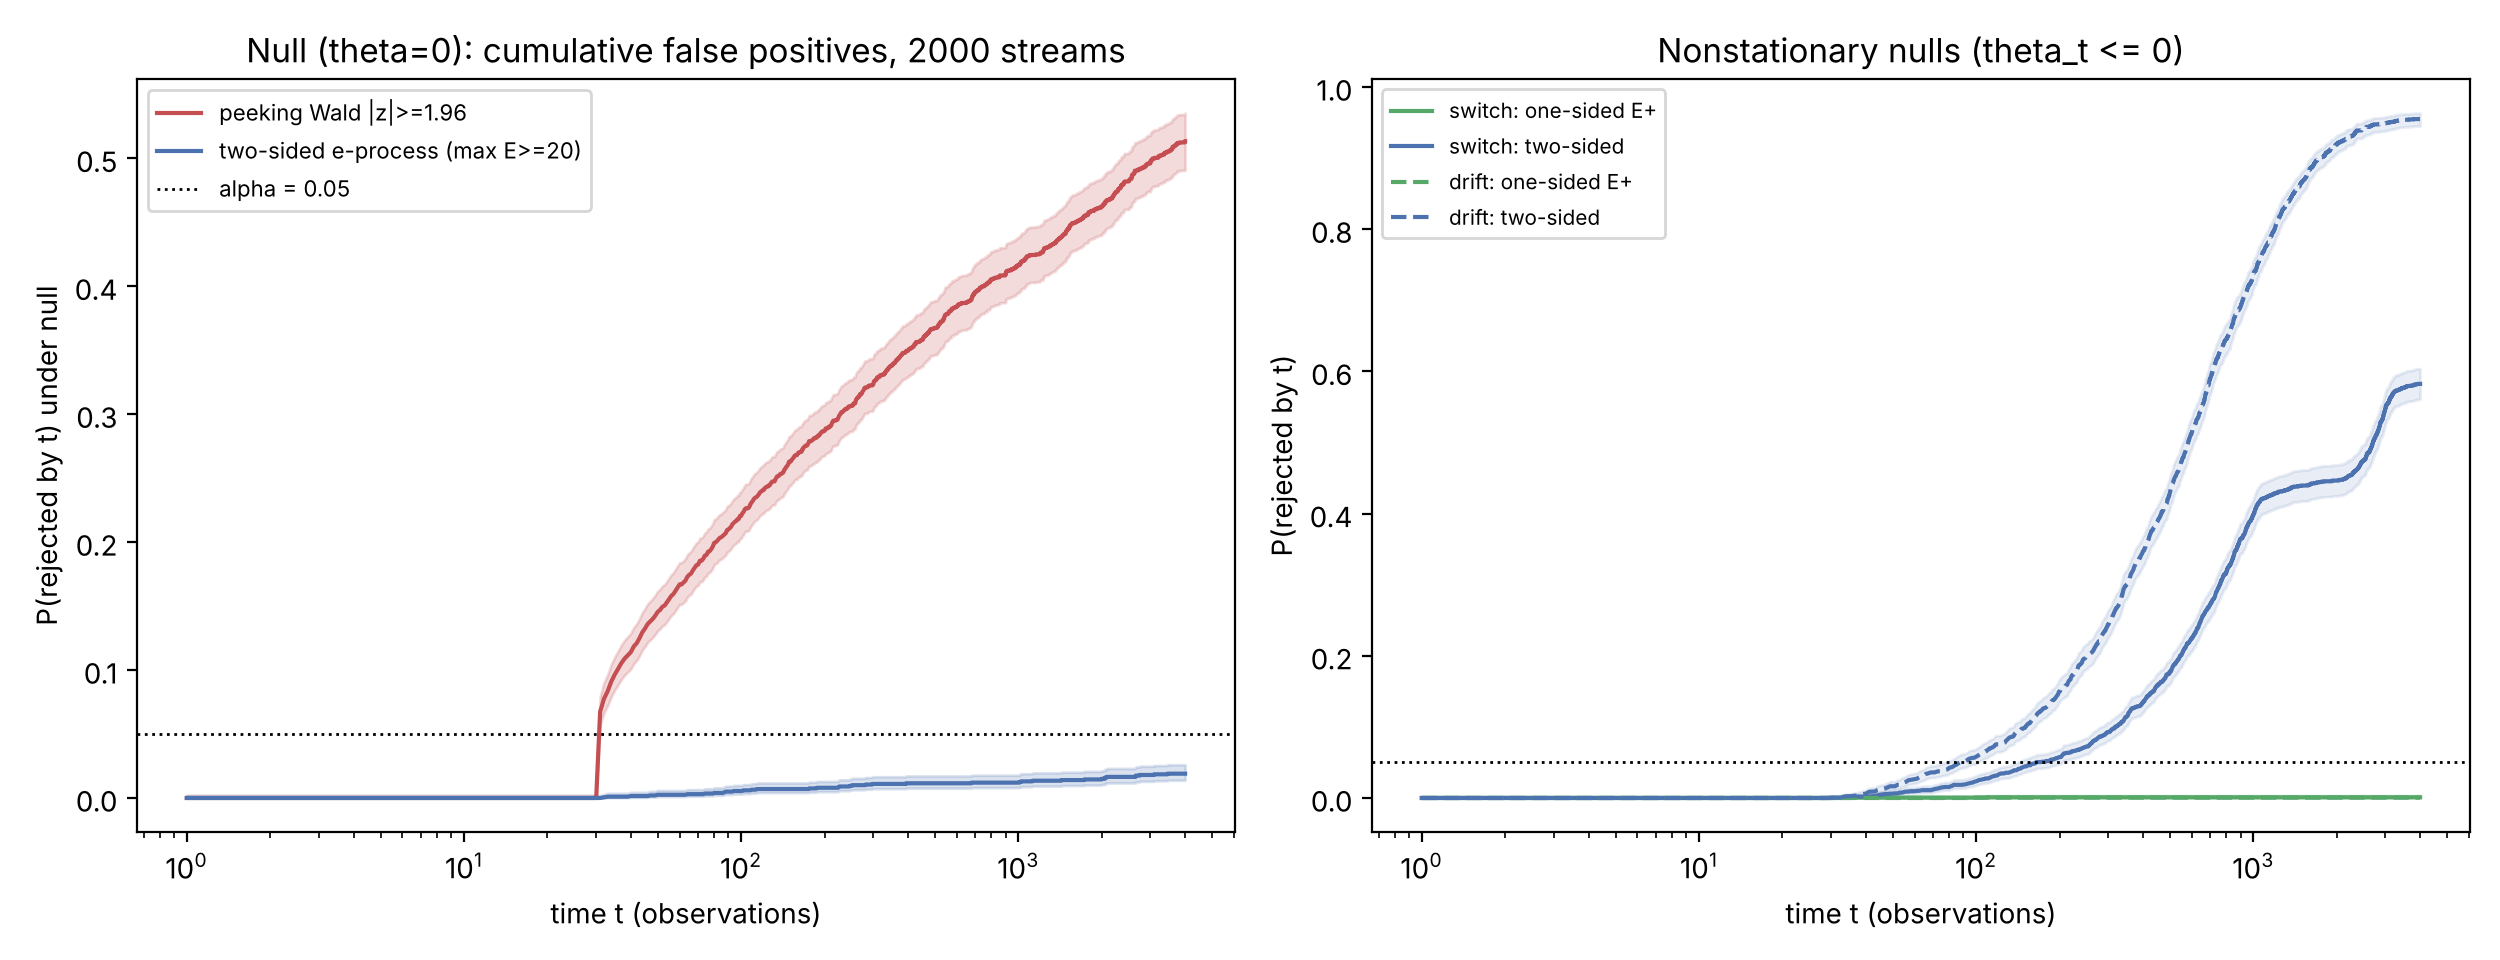
\includegraphics[width=0.98\textwidth]{figures/fig_interv_typeI.png}
\caption{\DIFaddFL{Interventional test. Left: cumulative false-positive rate under $\theta=0$ ($2000$ streams, shaded Wilson
bands) for a Wald test recomputed after every observation and the ANTE e-process. Right: under nonstationary
nulls with $\theta_t\le0$ the one-sided process stays at zero; the two-sided process rejects because its null is false at times}}\label{fig:interv}
\end{figure}

\paragraph{\DIFadd{The clipping argument fails; the new score does not.}} \DIFadd{We reproduce Example~\ref{ex:clipfail} by
simulation. With $\hat\sigma=1$ and clip level $5$, a plug-in bettor on i.i.d.\ draws from the example law
($\E s=-0.65$) reaches $E\ge20$ in $0.978$ of $2000$ streams ($[0.970,0.983]$, median $\log_{10}$ of the running
maximum $8.9$), although the raw null is true; with a data-dependent scale (the expanding root mean square) the same
law is not harmful ($0.004$), which is why such a defect can go unseen in simulations.
For the new score no such construction exists, because Theorem~\ref{thm:sgvalid} does not use the shape of the law of $s_t$}\DIFaddend .
Table~\DIFdelbegin \DIFdel{\ref{tab:datasets} lists the datasets; all code, data, and figure-generating
scripts are released}\footnote{%DIFDELCMD < \url{https://github.com/vinhqdang/REIGN_Regime-Enhanced-Intelligent-Granger-Network}
%DIFDELCMD < %%%
\DIFdel{(ANTE lives in the }\texttt{\DIFdel{sequential-synergy-causality/}} %DIFAUXCMD
\DIFdel{subdirectory).}}
%DIFAUXCMD
\addtocounter{footnote}{-1}%DIFAUXCMD
\DIFdel{(\S\ref{sec:decl}) so that every
number below is reproducible}\DIFdelend \DIFaddbegin \DIFadd{\ref{tab:stress} and Fig.~\ref{fig:stress} report ANTE-SG, the four-model score and the original test on twelve
VAR nulls ($T=2500$, $200$ replications each) built around the structure in the proof: heavy-tailed skewed
innovations, GARCH volatility clustering, source correlation up to $0.99$, cubic additive terms outside the feature span
with correlated sources, a sign break of the additive coefficients at $T/2$, own-nonlinearity, persistent ($\mathrm{AR}=0.9$)
sources, and short ($0.98$) and long ($0.999$) forgetting. ANTE-SG's false-rejection rate is at most $0.010$ ($2/200$) in every
scenario. The four-model score rejects $0.170$ $[0.124,0.228]$ of nulls under persistent sources (N10)
and $0.160$ $[0.110,0.227]$ at a realised source correlation of $0.20$ (Section~\ref{subsec:exp-corr}), although its raw mean score is negative in those cells (about $-0.004$ and $-0.02$). The rejections therefore do not
come from redundancy, which Proposition~\ref{prop:isolation}(b) predicts to make this score negative here; they show that the prequential null of the four-model score fails in finite samples for the learned forecasters (Remark~\ref{rem:notpop}), another reason to prefer the add-versus-joint contrast.
As an additional check against spurious-regression behaviour, independent AR(1) series with coefficient up to $0.999$ ($100$
replications each) give ANTE-SG false-rejection rates of at most $0.01$ ($1/100$ at $\varphi=0.97$, none otherwise) and none for the original test.
The limits of this evidence appear in Section~\ref{subsec:exp-fin} and the discussion: smooth, near-deterministic signals break it}\DIFaddend .

\begin{table}[h]
\caption{\DIFdelbeginFL \DIFdelFL{Datasets}\DIFdelendFL \DIFaddbeginFL \DIFaddFL{False-rejection rate (max $E\ge20$, $200$ replications, $T=2500$) under additive or no-synergy nulls, with Wilson
95\% intervals}\DIFaddendFL . \DIFdelbeginFL \DIFdelFL{Synthetic DGPs provide ground truth}\DIFdelendFL \DIFaddbeginFL \DIFaddFL{Scenarios (realised source correlation in brackets): N1 Gaussian ($0.36$)}\DIFaddendFL ; \DIFdelbeginFL \DIFdelFL{real panels are used for
the case study }\DIFdelendFL \DIFaddbeginFL \DIFaddFL{N2 Student-$t_3$ and skewed innovations ($0.36$); N3 $t_3$ }\DIFaddendFL and \DIFaddbeginFL \DIFaddFL{GARCH ($0.36$); N4, N5 strongly correlated sources ($0.96$, $0.99$);
N6, N7 additive cubic term outside }\DIFaddendFL the \DIFdelbeginFL \DIFdelFL{evidence-of-absence finding.}\DIFdelendFL \DIFaddbeginFL \DIFaddFL{feature span ($0.60$, $0.92$); N8 sign break of the additive coefficients at $T/2$;
N9 own-nonlinearity ($0.60$); N10 AR(0.9) sources ($0.60$); N11, N12 forgetting $0.98$, $0.999$}\DIFaddendFL }\DIFdelbeginFL %DIFDELCMD < \label{tab:datasets}
%DIFDELCMD < %%%
\DIFdelendFL \DIFaddbeginFL \label{tab:stress}
\DIFaddendFL \footnotesize
\DIFdelbeginFL %DIFDELCMD < \begin{tabular*}{\textwidth}{@{\extracolsep\fill}p{2.7cm}p{3.7cm}p{2.3cm}p{3.0cm}}
%DIFDELCMD < %%%
\DIFdelendFL \DIFaddbeginFL \begin{tabular*}{\textwidth}{@{\extracolsep\fill}lccc}
\DIFaddendFL \toprule
\DIFdelbeginFL \DIFdelFL{Dataset }%DIFDELCMD < & %%%
\DIFdelFL{Type }%DIFDELCMD < & %%%
\DIFdelFL{Size }%DIFDELCMD < & %%%
\DIFdelFL{Role }%DIFDELCMD < \\
%DIFDELCMD < \midrule
%DIFDELCMD < %%%
\DIFdelFL{Synthetic interventional }\DIFdelendFL \DIFaddbeginFL \DIFaddFL{Scenario }\DIFaddendFL & \DIFdelbeginFL \DIFdelFL{binary $A,B\!\to\!C$ (null/AND/XOR}\DIFdelendFL \DIFaddbeginFL \DIFaddFL{ANTE-SG (add-vs-joint}\DIFaddendFL ) & \DIFdelbeginFL \DIFdelFL{$\le4000$ steps }\DIFdelendFL \DIFaddbeginFL \DIFaddFL{four-model score }\DIFaddendFL & \DIFdelbeginFL \DIFdelFL{E1--E4 validity/power }\DIFdelendFL \DIFaddbeginFL \DIFaddFL{original clipped test }\DIFaddendFL \\
\DIFdelbeginFL \DIFdelFL{Synthetic common-factor VAR }\DIFdelendFL \DIFaddbeginFL \midrule
\DIFaddFL{N1--N2, N7, N9 }\DIFaddendFL & \DIFdelbeginFL \DIFdelFL{additive / $A^2$ / $A\!\cdot\!B$ + factor }\DIFdelendFL \DIFaddbeginFL \DIFaddFL{$0/200$ each }\DIFaddendFL & \DIFdelbeginFL \DIFdelFL{$T\approx2500$--$4000$ }\DIFdelendFL \DIFaddbeginFL \DIFaddFL{$0/200$ each }\DIFaddendFL & \DIFdelbeginFL \DIFdelFL{S1--S4, benchmark AUC }\DIFdelendFL \DIFaddbeginFL \DIFaddFL{$0/200$ each }\DIFaddendFL \\
\DIFdelbeginFL \DIFdelFL{US sector-ETF }\DIFdelendFL \DIFaddbeginFL \DIFaddFL{N3 (heavy tails }\DIFaddendFL + \DIFdelbeginFL \DIFdelFL{macro panel }%DIFDELCMD < & %%%
\DIFdelFL{16 daily assets }%DIFDELCMD < & %%%
\DIFdelFL{2512 days (2016--26}\DIFdelendFL \DIFaddbeginFL \DIFaddFL{GARCH}\DIFaddendFL ) & \DIFdelbeginFL \DIFdelFL{real scans, portfolio variance }%DIFDELCMD < \\
%DIFDELCMD < %%%
\DIFdelFL{World equity indices }%DIFDELCMD < & %%%
\DIFdelFL{6 daily indices }\DIFdelendFL \DIFaddbeginFL \DIFaddFL{$1/200$ }\DIFaddendFL & \DIFdelbeginFL \DIFdelFL{2138 days }\DIFdelendFL \DIFaddbeginFL \DIFaddFL{$0/200$ }\DIFaddendFL & \DIFdelbeginFL \DIFdelFL{cross-region synergy }\DIFdelendFL \DIFaddbeginFL \DIFaddFL{$0/200$ }\DIFaddendFL \\
\DIFdelbeginFL \DIFdelFL{``Famous stocks'' basket }\DIFdelendFL \DIFaddbeginFL \DIFaddFL{N4 ($\rho=.95$) }\DIFaddendFL & \DIFdelbeginFL \DIFdelFL{13 daily / 12 hourly }\DIFdelendFL \DIFaddbeginFL \DIFaddFL{$1/200$ }\DIFaddendFL & \DIFdelbeginFL \DIFdelFL{2512 d / 3328 h }\DIFdelendFL \DIFaddbeginFL \DIFaddFL{$0/200$ }\DIFaddendFL & \DIFdelbeginFL \DIFdelFL{plain-language scans }\DIFdelendFL \DIFaddbeginFL \DIFaddFL{$0/200$ }\DIFaddendFL \\
\DIFdelbeginFL \DIFdelFL{Crypto (intraday}\DIFdelendFL \DIFaddbeginFL \DIFaddFL{N5 ($\rho=.99$}\DIFaddendFL ) & \DIFdelbeginFL \DIFdelFL{10 coins, hourly }\DIFdelendFL \DIFaddbeginFL \DIFaddFL{$2/200$ $[0.003,0.036]$ }\DIFaddendFL & \DIFdelbeginFL \DIFdelFL{16}%DIFDELCMD < {%%%
\DIFdelFL{,}%DIFDELCMD < }%%%
\DIFdelFL{761 hours }\DIFdelendFL \DIFaddbeginFL \DIFaddFL{$0/200$ }\DIFaddendFL & \DIFdelbeginFL \DIFdelFL{high-sample group scan }\DIFdelendFL \DIFaddbeginFL \DIFaddFL{$0/200$ }\DIFaddendFL \\
\DIFdelbeginFL \DIFdelFL{Climate teleconnections }\DIFdelendFL \DIFaddbeginFL \DIFaddFL{N6, N8, N11, N12 }\DIFaddendFL & \DIFdelbeginFL \DIFdelFL{6 monthly indices }\DIFdelendFL \DIFaddbeginFL \DIFaddFL{$1/200$ each }\DIFaddendFL & \DIFdelbeginFL \DIFdelFL{865 months }\DIFdelendFL \DIFaddbeginFL \DIFaddFL{$0/200$ each }\DIFaddendFL & \DIFdelbeginFL \DIFdelFL{non-finance control }\DIFdelendFL \DIFaddbeginFL \DIFaddFL{$0/200$ each }\DIFaddendFL \\
\DIFdelbeginFL \DIFdelFL{Turbulence energy cascade }\DIFdelendFL \DIFaddbeginFL \DIFaddFL{N10 (persistent sources) }\DIFaddendFL & \DIFdelbeginFL \DIFdelFL{4 scale-resolved signals }\DIFdelendFL \DIFaddbeginFL \DIFaddFL{$0/200$ }\DIFaddendFL & \DIFdelbeginFL \DIFdelFL{21}%DIFDELCMD < {%%%
\DIFdelFL{,}%DIFDELCMD < }%%%
\DIFdelFL{760 samples }\DIFdelendFL \DIFaddbeginFL \DIFaddFL{$\mathbf{34/200}$ $[0.124,0.228]$ }\DIFaddendFL & \DIFdelbeginFL \textbf{\DIFdelFL{positive}} %DIFAUXCMD
\DIFdelFL{3-way (physics) }\DIFdelendFL \DIFaddbeginFL \DIFaddFL{$0/200$ }\DIFaddendFL \\
\botrule
\end{tabular*}
\end{table}

\DIFdelbegin \subsection{\DIFdel{Anytime-validity, discrimination, and power}}%DIFAUXCMD
\addtocounter{subsection}{-1}%DIFAUXCMD
%DIFDELCMD < \label{subsec:exp-validity}
%DIFDELCMD < %%%
\DIFdelend \DIFaddbegin \begin{figure}[h]
\centering
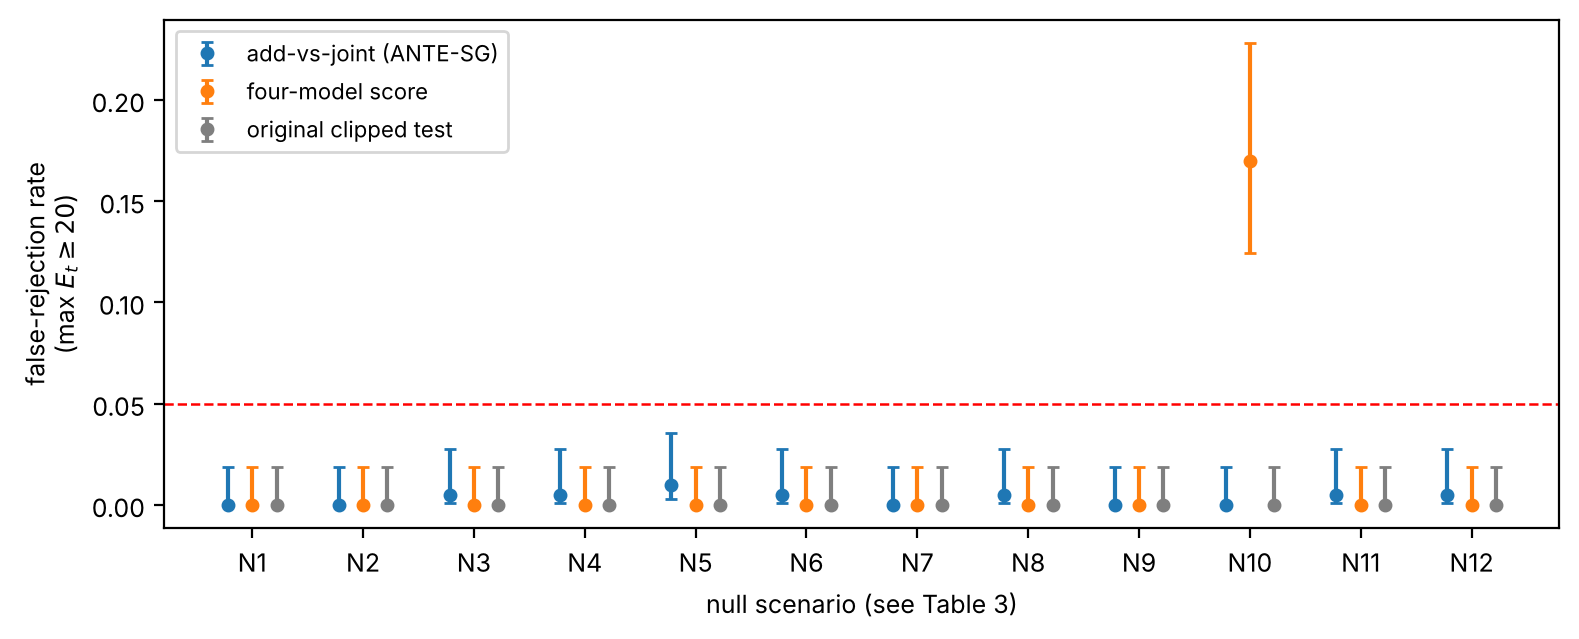
\includegraphics[width=0.98\textwidth]{figures/fig_stress.png}
\caption{\DIFaddFL{False-rejection rate of the three procedures under the twelve nulls of Table~\ref{tab:stress}
(Wilson 95\% intervals; dashed line: $\alpha=0.05$)}}\label{fig:stress}
\end{figure}
\DIFaddend 

\paragraph{\DIFdelbegin \DIFdel{Type-I error under continuous monitoring}\DIFdelend \DIFaddbegin \DIFadd{Power and detection time}\DIFaddend .} \DIFdelbegin \DIFdel{The central claim of
Corollary~\ref{cor:anytime} is that ANTE may be monitored after every observation
without inflating its error rate. We test this directly. On $2000$ independent null
streams of length $4000$ (a balanced $2\times2$ interventional design with
$\theta=0$}\DIFdelend \DIFaddbegin \DIFadd{For a bilinear mechanism $Y_t=cA_{t-1}B_{t-1}+0.2A_{t-1}+0.3Z_t+\varepsilon_t$
(realised source correlation $0.36$, $T=2500$, $500$ replications per $c$}\DIFaddend ), \DIFdelbegin \DIFdel{we record, at every step $t$, whether the running e-process has ever
crossed $1/\alpha$. ANTE's monitored false-positive rate is $\mathbf{0.031}$ and stays uniformly below the nominal $\alpha=0.05$ across the }\emph{\DIFdel{entire}} %DIFAUXCMD
\DIFdel{horizon, consistent with the slight conservativeness Ville's inequality induces.
The
comparison procedure is the one a practitioner is most likely to use by default: a
fixed-$n$ Wald $z$-test }\DIFdelend \DIFaddbegin \DIFadd{ANTE-SG's power is $0.07$ $[0.05,0.09]$ at $c=0.1$, $0.78$ $[0.74,0.81]$ at $c=0.2$ and $\ge0.998$ }\DIFaddend for
\DIFdelbegin \DIFdel{$\theta=0$, recomputed and re-consulted after each new
observation (Remark~\ref{rem:peeking}). Its cumulative false-positive rate climbs
monotonically with the number of looks---past $0.17$ by $t=50$, past $0.40$ by
$t=600$, and reaching $\mathbf{0.505}$ by the end of the stream, a tenfold
violation of the nominal level }\DIFdelend \DIFaddbegin \DIFadd{$c\ge0.3$, with false-rejection $0.000$ at $c=0$; the original test reaches only $0.34$ at $c=0.2$ and $0.60$--$0.69$ for $c\ge0.3$.
At the family-wise thresholds the picture is less favourable (150 replications): at $c=0.2$ power falls from $0.83$ at $1/\alpha$ to $0.06$ at $m/\alpha$ with $m=660$ and $0.03$ with $m=4400$; at $c=0.3$ it is $0.99$, $0.77$ and $0.61$, and at $c=0.45$ it is $1.00$ throughout.
The median detection time of ANTE-SG falls from $1346$ $(1256,1438)$ at $c=0.2$ to $140$ $(132,147)$ at $c=0.9$ (bootstrap intervals), directionally consistent with the $\delta^{-2}$ scaling of Proposition~\ref{prop:latency}
(the effect grows $4.5$-fold while the median detection time falls $9.6$-fold; the proposition is for an oracle bet and a different score, and we do not claim the bound is tight). For the original test, power dips at the largest $c$ ($0.69\to0.63$, within Monte Carlo error: the intervals overlap) and latency rises ($1095\to1473$, outside Monte Carlo error because that test's scale estimator degrades);
ANTE-SG's power is monotone within its intervals and its latency non-increasing in $c\ge0.2$ }\DIFaddend (Fig.~\DIFdelbegin \DIFdel{\ref{fig:type1}). This is the empirical face
of the theory: optional-stopping validity is not a technicality but the difference
between a $5\%$ and a
$50\%$ error rate}\DIFdelend \DIFaddbegin \DIFadd{\ref{fig:power}). Theorem~\ref{thm:consistency} and Proposition~\ref{prop:latency} apply to ANTE-SG with $\psi_t$ replaced by the normalised score $u_t$ ($c=1$) and a
fixed bet; the plug-in bet is evaluated here only empirically}\DIFaddend .

\begin{figure}[h]
\centering
\DIFdelbeginFL %DIFDELCMD < 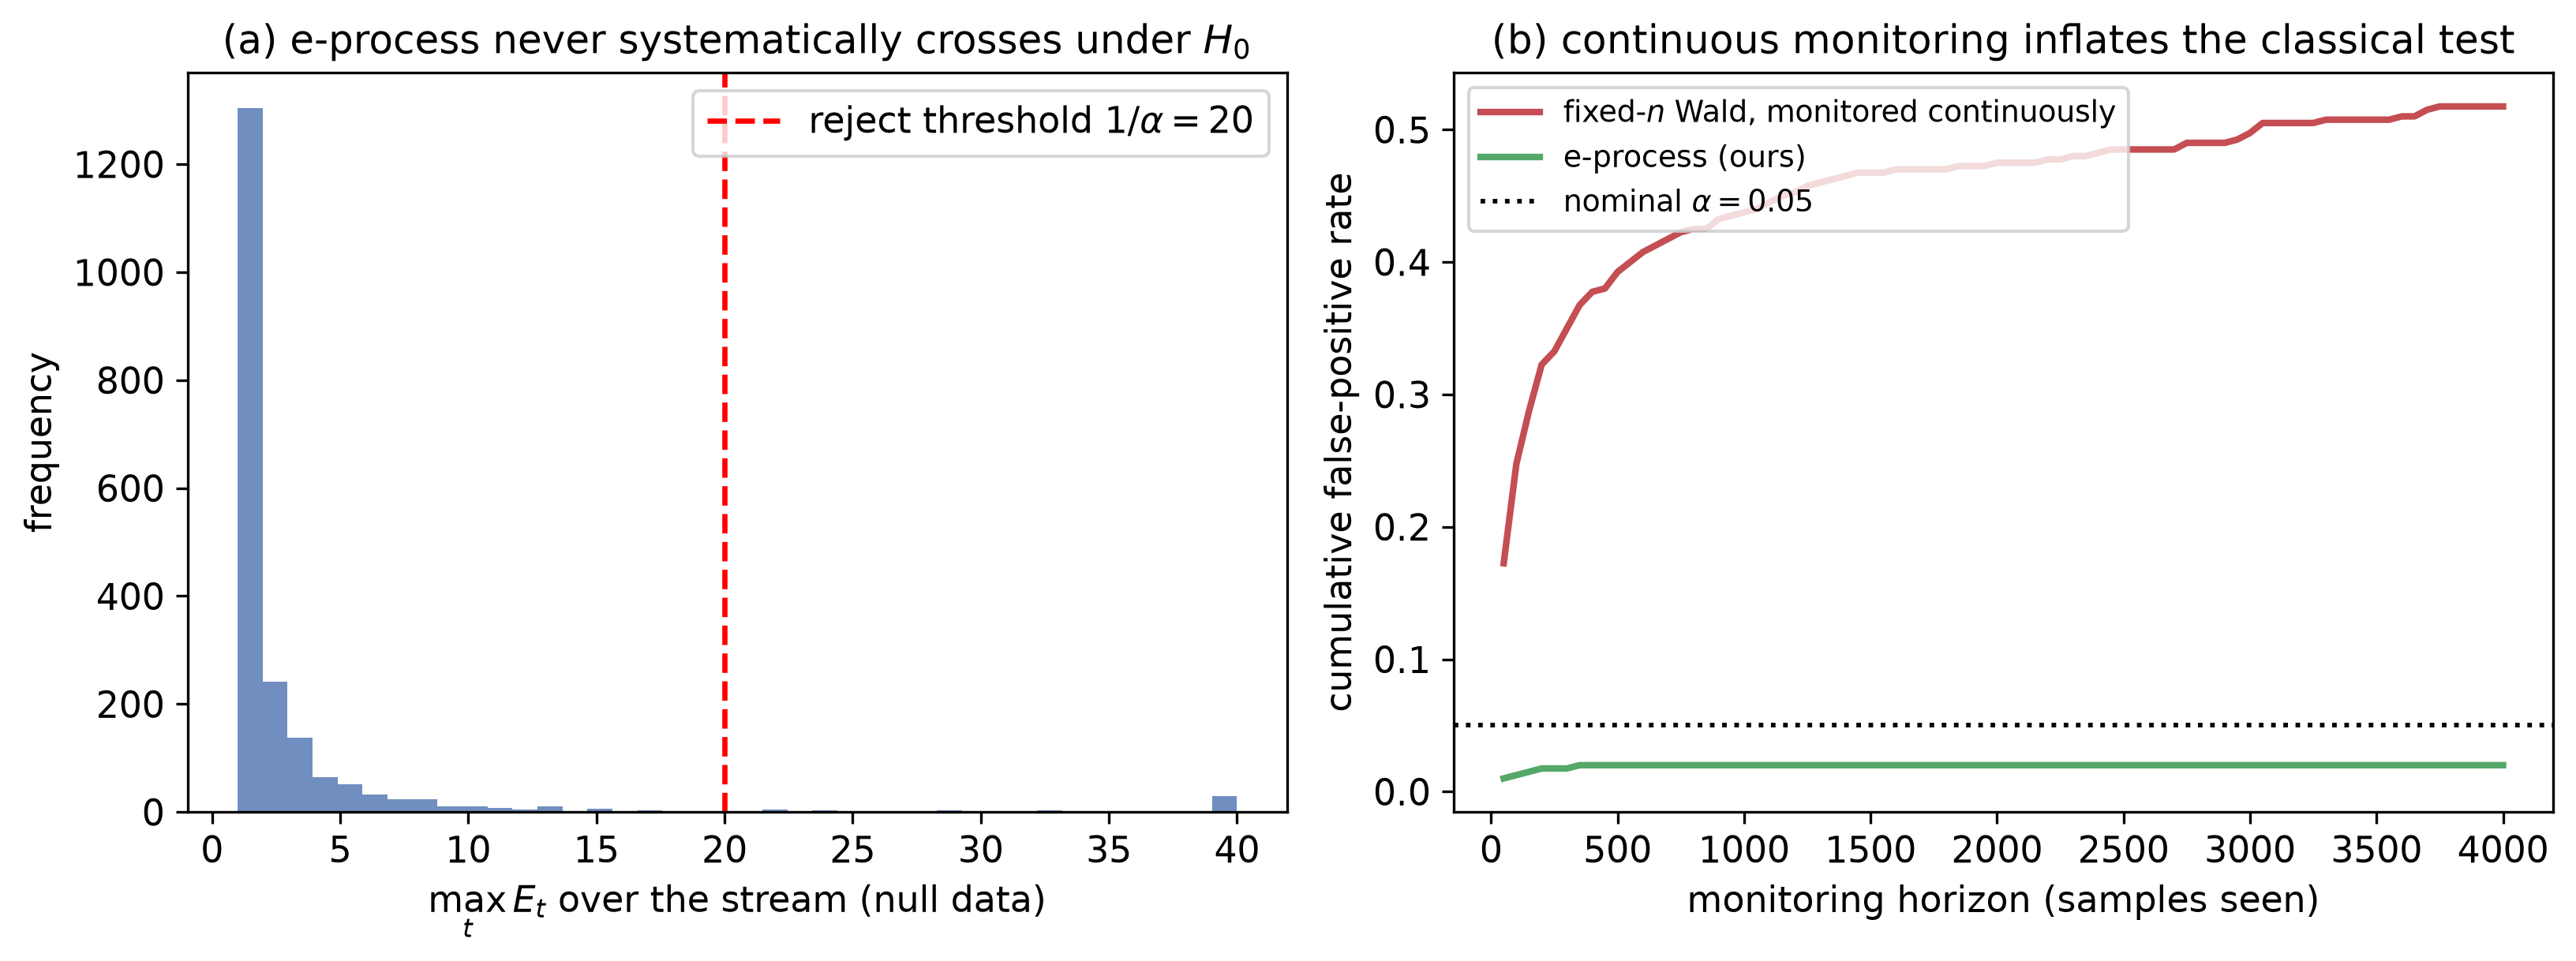
\includegraphics[width=0.9\textwidth]{figures/e1_type_one_error.png}
%DIFDELCMD < %%%
\DIFdelendFL \DIFaddbeginFL 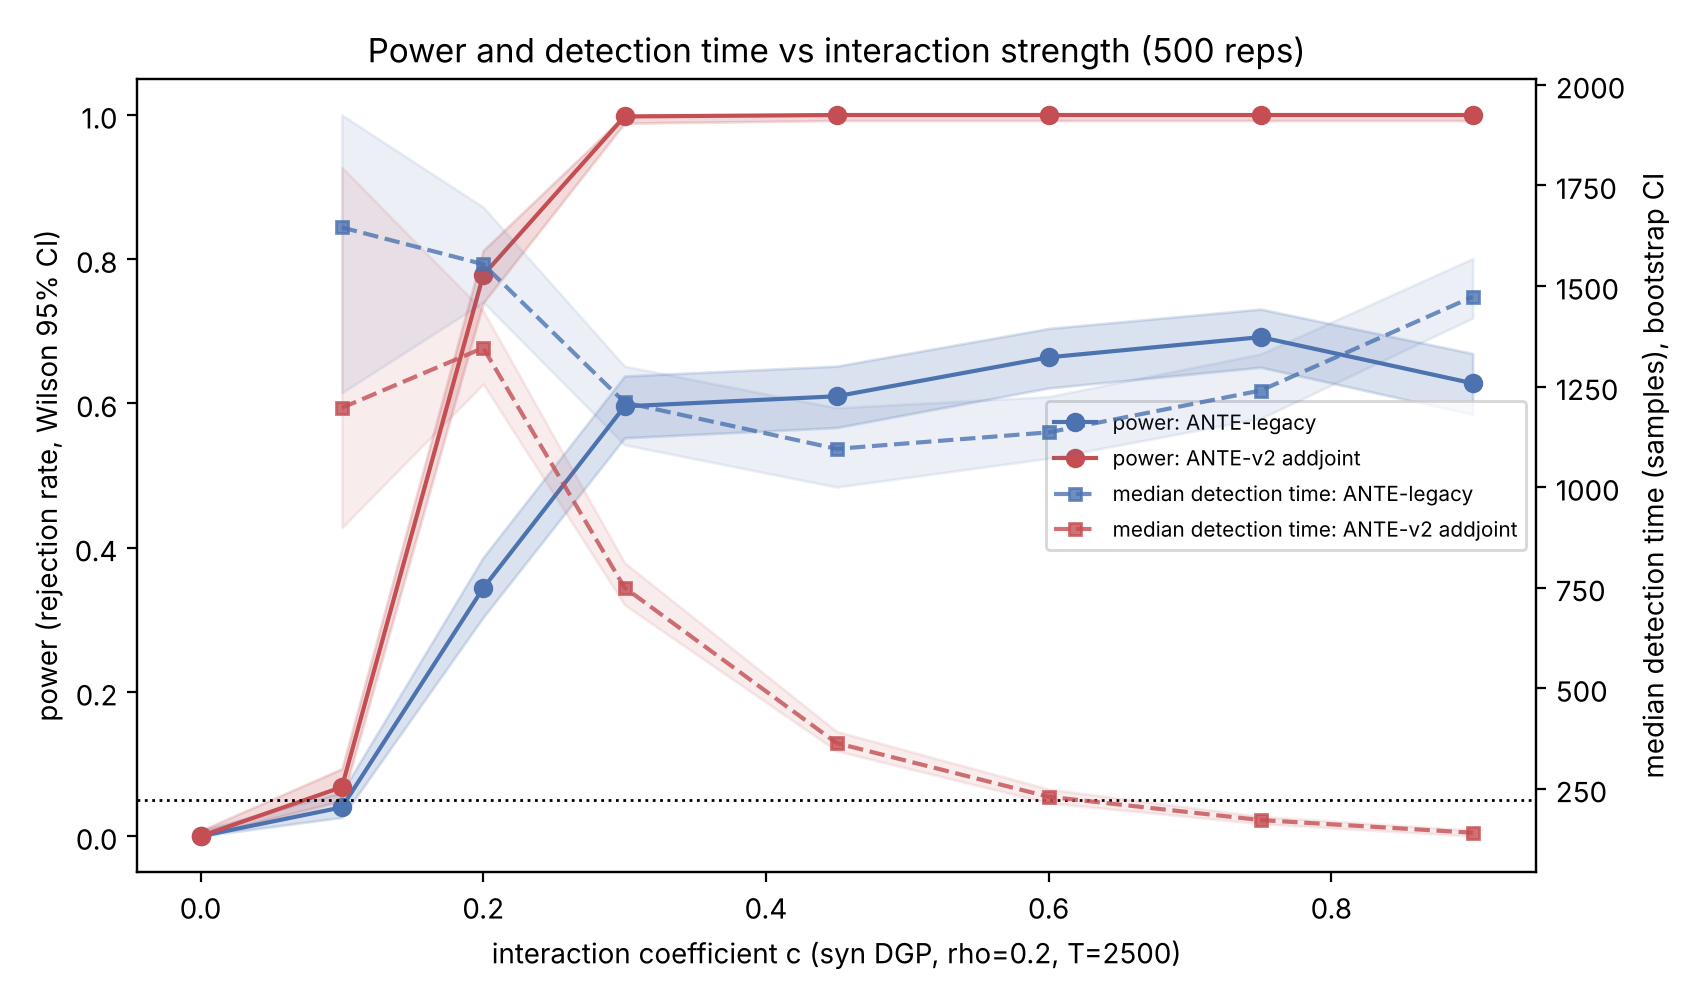
\includegraphics[width=0.85\textwidth]{figures/fig_power.png}
\DIFaddendFL \caption{\DIFdelbeginFL \DIFdelFL{Anytime-valid Type-I control. The ANTE e-process }\DIFdelendFL \DIFaddbeginFL \DIFaddFL{Power }\DIFaddendFL (\DIFdelbeginFL \DIFdelFL{lower curve}\DIFdelendFL \DIFaddbeginFL \DIFaddFL{solid, left axis}\DIFaddendFL ) \DIFdelbeginFL \DIFdelFL{keeps the
monitored false-positive rate below the nominal $\alpha=0.05$ uniformly over }\DIFdelendFL \DIFaddbeginFL \DIFaddFL{and median detection time (dashed, right axis) versus }\DIFaddendFL the \DIFdelbeginFL \DIFdelFL{stream}\DIFdelendFL \DIFaddbeginFL \DIFaddFL{interaction coefficient}\DIFaddendFL , \DIFdelbeginFL \DIFdelFL{while a continuously monitored fixed-sample Wald test }\DIFdelendFL \DIFaddbeginFL \DIFaddFL{with Wilson and bootstrap bands }\DIFaddendFL (\DIFdelbeginFL \DIFdelFL{upper curve}\DIFdelendFL \DIFaddbeginFL \DIFaddFL{$500$ replications per point}\DIFaddendFL )\DIFdelbeginFL \DIFdelFL{inflates past $0.5$. Validity holds at every stopping time}\DIFdelendFL , \DIFdelbeginFL \DIFdelFL{not merely at a
pre-committed horizon}\DIFdelendFL \DIFaddbeginFL \DIFaddFL{for the original test and ANTE-SG}\DIFaddendFL }\DIFdelbeginFL %DIFDELCMD < \label{fig:type1}
%DIFDELCMD < %%%
\DIFdelendFL \DIFaddbeginFL \label{fig:power}
\DIFaddendFL \end{figure}

\DIFdelbegin \paragraph{\DIFdel{Discrimination: interaction versus joint dependence.}} %DIFAUXCMD
\addtocounter{paragraph}{-1}%DIFAUXCMD
\DIFdel{Validity is worthless if the test cannot tell real synergy from its two impostors. We generate
three common-factor VAR DGPs ($T\approx2500$, $n_{\mathrm{rep}}=300$) , each with a
shared market factor so that both sources are individually predictive of the
target: (a)}\emph{\DIFdel{additive}}%DIFAUXCMD
\DIFdel{, $Y_t$ depends on lagged $A$ and lagged $B$
separately; (b)}\emph{\DIFdel{own-nonlinear}}%DIFAUXCMD
\DIFdel{, $Y_t$ depends on $A_{t-1}^2$---a curved but
single-source mechanism; and (c)}\emph{\DIFdel{synergistic}}%DIFAUXCMD
\DIFdel{, $Y_t$ depends on the
cross-product $A_{t-1}B_{t-1}$. ANTE-SG rejects the additive DGP at rate
$\mathbf{0.00}$ and the own-nonlinear DGP at $\mathbf{0.01}$---both at or below
$\alpha$---while firing on genuine cross-interaction at $\mathbf{0.71}$. This is
the practical content of Proposition~\ref{prop:isolation}: the additive and single-source curved mechanisms are absorbed by the marginal predictors and are
not mistaken for synergy, and only irreducible $A\times B$ structure moves the capital. As \S\ref{subsec:exp-benchmark} shows, the information-theoretic
estimators fail exactly this test, reporting spurious positive synergy on the
additive DGP. }\DIFdelend \DIFaddbegin \subsection{\DIFadd{Correlated sources and nonlinear alternatives}}\label{subsec:exp-corr}
\DIFaddend 

\DIFdelbegin \paragraph{\DIFdel{Power and latency.}} %DIFAUXCMD
\addtocounter{paragraph}{-1}%DIFAUXCMD
\DIFdel{We then sweep the interaction coefficient from $0$
}\DIFdelend \DIFaddbegin \DIFadd{A natural question is what happens when sources are strongly correlated while the mechanism is additive. We vary the
source correlation (realised correlation $0.20$ }\DIFaddend to \DIFaddbegin \DIFadd{$0.99$) for an additive mechanism and for an interaction of strength }\DIFaddend $0.9$ (\DIFdelbegin \DIFdel{$n_{\mathrm{rep}}=250$}\DIFdelend \DIFaddbegin \DIFadd{$150$ replications per cell).
ANTE-SG's false-rejection rate is $0.000$ in all seven cells ($[0,0.025]$). The mean raw four-model score decreases from $-0.02$ at correlation $0.2$ to $-1.04$
at $0.99$ on the additive mechanism, as the redundancy term predicts, whereas the add-versus-joint score stays between $-0.04$ and $-0.007$ (Fig.~\ref{fig:corr}). The
cost of isolating the interaction is power when the two sources become nearly collinear: ANTE-SG's power against the interaction is $1.00$ up to correlation $0.68$}\DIFaddend , \DIFdelbegin \DIFdel{$T=2500$) and record both the rejection rate and, among rejections, the median detection time.
Power rises monotonically with synergy
strength ($0\to0.20\to0.47\to0.68\to0.74\to0.79$) }\DIFdelend \DIFaddbegin \DIFadd{$0.97$ $[0.92,0.99]$ at $0.84$}\DIFaddend ,
\DIFdelbegin \DIFdel{and---the sequential signature
that no fixed-sample test exhibits---median detection latency }\emph{\DIFdel{falls}} %DIFAUXCMD
\DIFdel{as the signal grows: strongsynergy is not merely detected more often but detected
}\emph{\DIFdel{sooner}} %DIFAUXCMD
\DIFdel{(Fig.~\ref{fig:power}). This is exactly the
$\tau_\alpha\lesssim\log(1/\alpha)/\delta^2$ behaviour of
Proposition~\ref{prop:latency}: the stronger the effect $\delta$, }\DIFdelend \DIFaddbegin \DIFadd{$0.19$ $[0.13,0.26]$ at $0.92$, $0.007$ at $0.96$ and $0$ at $0.99$. When $A\approx B$ the cross-product $AB$ is nearly collinear with the own-quadratic features
$A^2,B^2$ and }\DIFaddend the \DIFdelbegin \DIFdel{fewer
observations the sceptic needs to bankrupt the null . }\DIFdelend \DIFaddbegin \DIFadd{interaction is not identifiable; this is a property of the problem, not an artefact, and it bounds what any add-versus-joint test can claim for near-collinear assets
(for example for two equity sector funds). }\DIFaddend The \DIFdelbegin \DIFdel{plateau near
$0.8$ at the largest coefficients reflects the finite horizon $T=2500$ combined
with the
conservative warm-up, not a ceiling of the method.
}\DIFdelend \DIFaddbegin \DIFadd{four-model score loses power sooner ($0.013$ at correlation $0.68$) because its redundancy term turns negative, and the original test is the least powerful
throughout ($0.73$ at correlation $0.2$, $0.31$ at $0.44$, $0$ from $0.68$).
}\DIFaddend 

\begin{figure}[h]
\centering
\DIFdelbeginFL %DIFDELCMD < 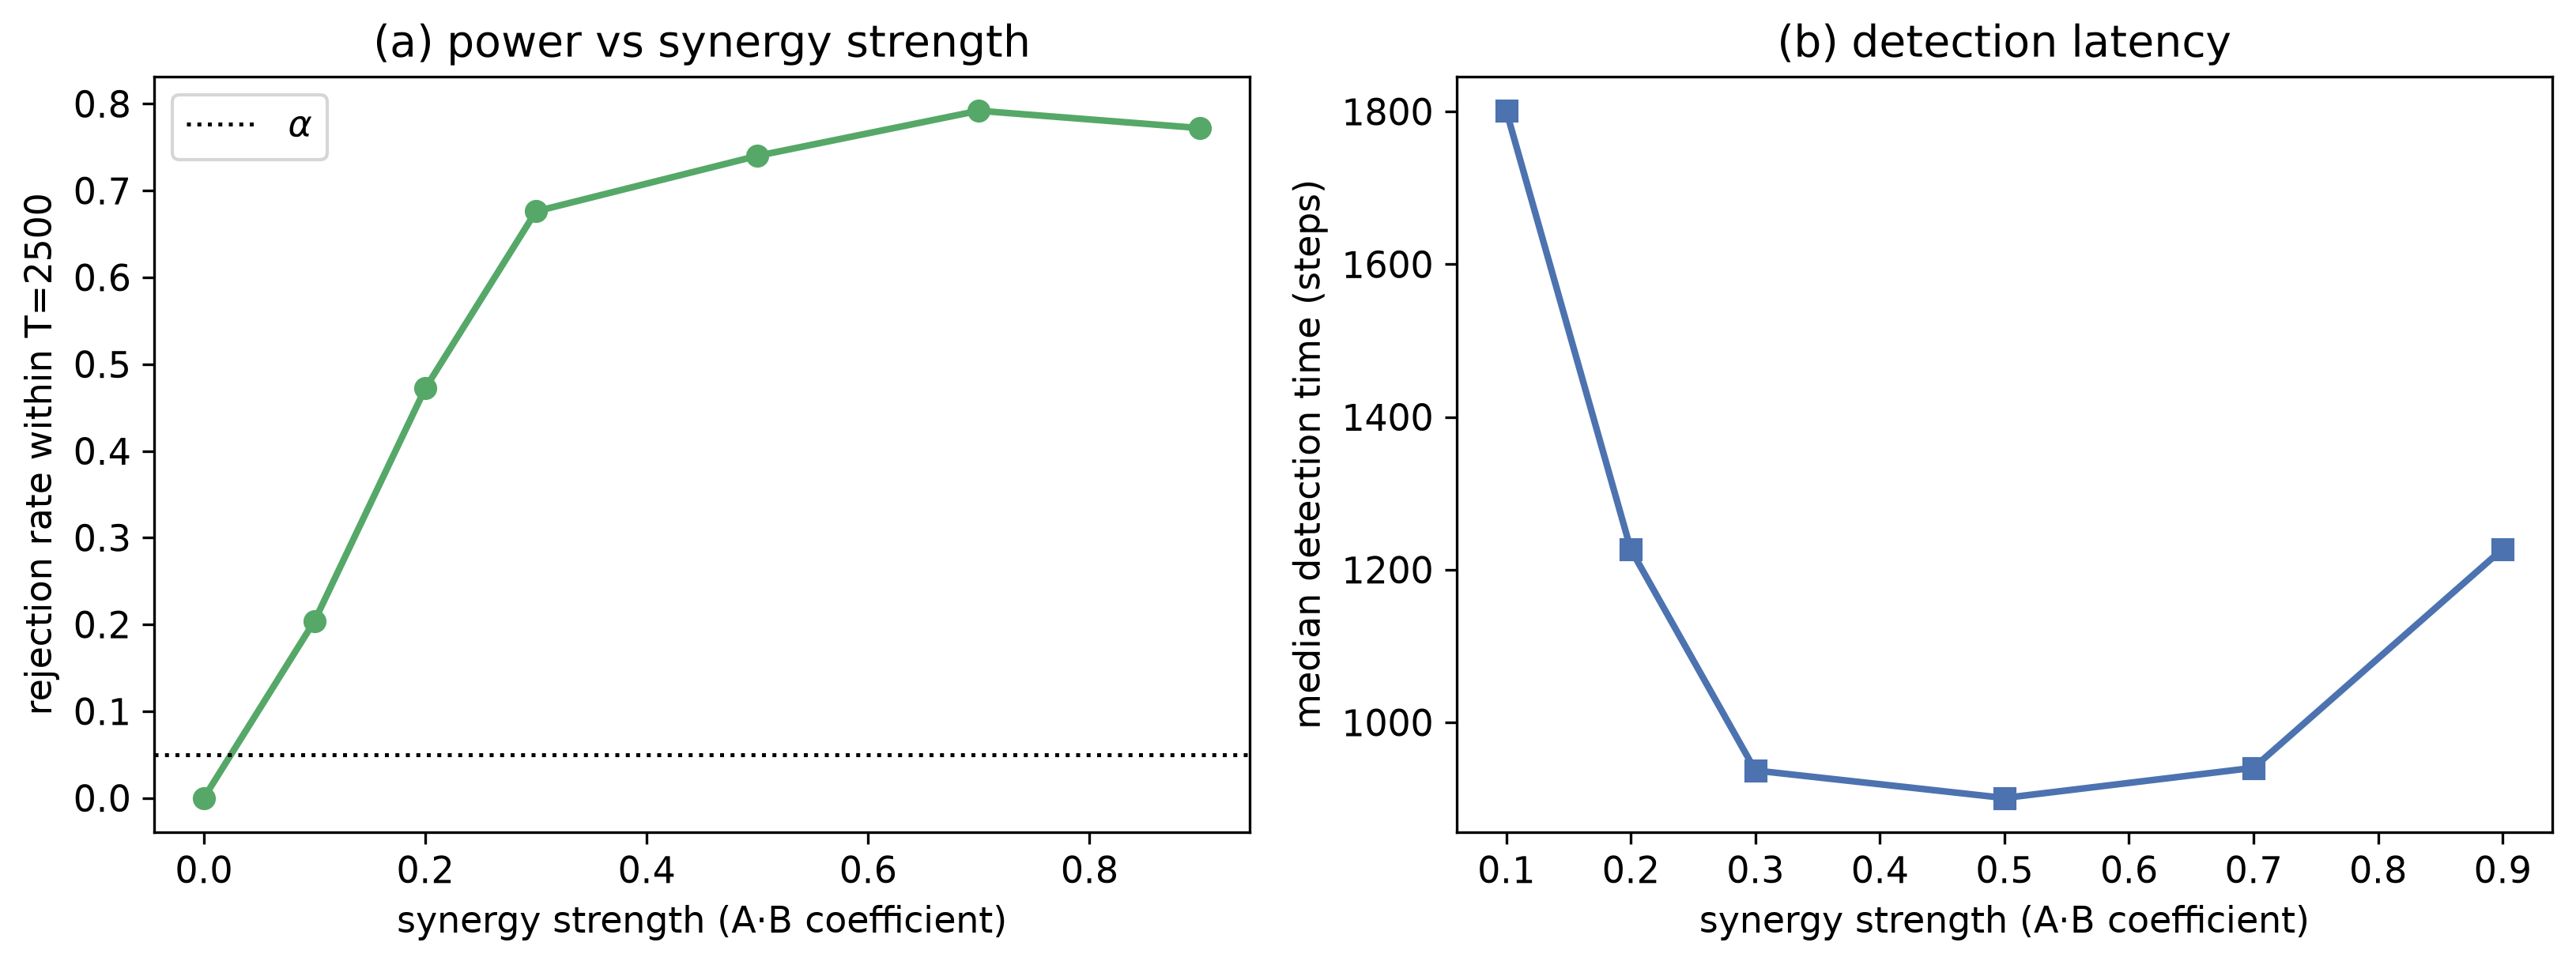
\includegraphics[width=0.9\textwidth]{figures/sg_s3_power_latency.png}
%DIFDELCMD < %%%
%DIFDELCMD < \caption{%
{%DIFAUXCMD
\DIFdelFL{Power (left axis) and median detection time (right axis) versus synergy
strength. Power increases monotonically toward $\approx0.8$; detection latency
shrinks as the signal grows, matching the $\log(1/\alpha)/\delta^2$ scaling of
Proposition~\ref{prop:latency}}}%DIFAUXCMD
%DIFDELCMD < \label{fig:power}
%DIFDELCMD < %%%
\DIFdelendFL \DIFaddbeginFL 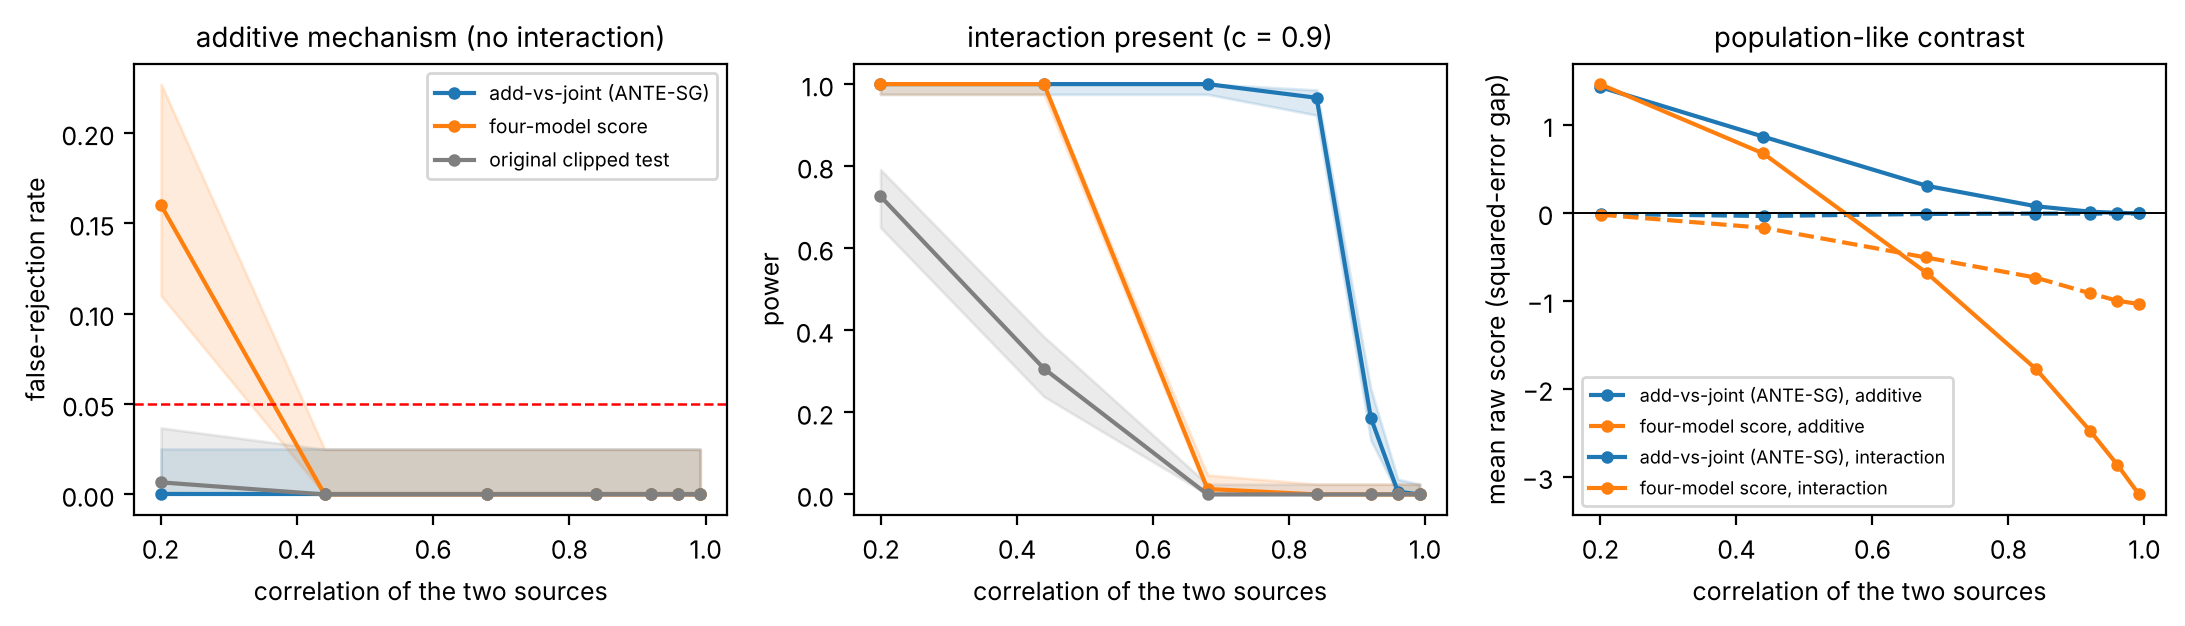
\includegraphics[width=\textwidth]{figures/fig_corr.png}
\caption{\DIFaddFL{Correlated sources. Left: false-rejection rate under an additive mechanism. Centre: power against an interaction of strength $0.9$.
Right: mean raw score (squared-error gap); the four-model score becomes strongly negative with redundancy while the add-versus-joint score stays near zero. Bands: Wilson 95\% intervals ($150$ replications)}}\label{fig:corr}
\DIFaddendFL \end{figure}

\DIFaddbegin \paragraph{\DIFadd{The test is only as nonparametric as its predictor class.}} \DIFadd{The dictionary used above (own linear and squared lags plus
cross-products) detects a bilinear and a bounded }\emph{\DIFadd{tanh$\times$tanh}} \DIFadd{or }\emph{\DIFadd{sin}} \DIFadd{interaction ($100$ replications, power $1.00$ each) because their projections onto the cross-product are strong, but it
fails on $Y_t=0.9A_{t-1}^2B_{t-1}+\dots$, an interaction outside its span: power $0.03$ $[0.01,0.08]$ at $T=2500$ and again at $T=5000$.
Replacing the dictionary by a random-Fourier-feature map \mbox{%DIFAUXCMD
\citep{rahimirecht2007} }\hskip0pt%DIFAUXCMD
(fifteen features per source and fifteen for the pair, with fixed seed-independent frequencies) detects it with power $1.00$ $[0.96,1.00]$
at both sample sizes, while its false-rejection rate on the additive null remains $0.00$ $[0,0.04]$. The framework (the betting construction and Theorem~\ref{thm:sgvalid}) accommodates any predictable forecaster pair; the
RLS-on-polynomials instantiation is one choice, and we describe it as a ``model-based prequential time-series implementation of an anytime-valid testing framework'' rather than as a nonparametric test.
}

\DIFaddend \subsection{Benchmark against \DIFdelbegin \DIFdel{2024--2026 methods}\DIFdelend \DIFaddbegin \DIFadd{batch synergy estimators}\DIFaddend }\label{subsec:exp-benchmark}

\DIFdelbegin \DIFdel{A method's value is relative, so we compare ANTE directly against the strongest
available synergy quantifiers: SURD \mbox{%DIFAUXCMD
\citep{surd2024}}\hskip0pt%DIFAUXCMD
and }\DIFdelend \DIFaddbegin \DIFadd{SURD \mbox{%DIFAUXCMD
\citep{surd2024}}\hskip0pt%DIFAUXCMD
, }\DIFaddend PEID \citep{peid2026}, \DIFdelbegin \DIFdel{the
2024--2026 state of the art; }\DIFdelend Williams--Beer PID \citep{williams2010}\DIFdelbegin \DIFdel{; }\DIFdelend \DIFaddbegin \DIFadd{, }\DIFaddend Gaussian interaction information \citep{mcgill1954} \DIFdelbegin \DIFdel{; }\DIFdelend and
O-information \citep{rosas2019} \DIFdelbegin \DIFdel{. To
guard against implementation error, each }\DIFdelend \DIFaddbegin \DIFadd{are }\emph{\DIFadd{estimators}} \DIFadd{of information-theoretic synergy, a different estimand from the predictive contrast tested here. We therefore report the comparison as one of
complementary tools. Each }\DIFaddend baseline was first \DIFdelbegin \DIFdel{validated }\DIFdelend \DIFaddbegin \DIFadd{checked }\DIFaddend against its own source\DIFdelbegin \DIFdel{. On the canonical logic gates }\DIFdelend \DIFaddbegin \DIFadd{: }\DIFaddend our PEID implementation returns \DIFdelbegin \DIFdel{$\mathrm{Syn}=1.00$ for XOR (pure synergy) }\DIFdelend \DIFaddbegin \DIFadd{$1.00$ for XOR }\DIFaddend and $0.19$ for AND \DIFdelbegin \DIFdel{, matching the paper's
reported }\DIFdelend \DIFaddbegin \DIFadd{(published value }\DIFaddend $0.189$\DIFdelbegin \DIFdel{; }\DIFdelend \DIFaddbegin \DIFadd{), }\DIFaddend PID and SURD agree on XOR ($1.00$) and
give $0.50$ on AND\DIFdelbegin \DIFdel{; and all methods }\DIFdelend \DIFaddbegin \DIFadd{, and all }\DIFaddend return $\approx0$ on a redundant copy and on independent noise. \DIFdelbegin \DIFdel{SURD
itself was run }\DIFdelend \DIFaddbegin \DIFadd{Settings (not tuned per method): SURD with six equal-mass bins per variable on the lagged triple $(A_{t-1},B_{t-1},Y_t)$ }\DIFaddend through
the authors' released code\DIFdelbegin \DIFdel{. This calibration lets us
attribute any downstream difference to the methods, not to our re-implementations}\DIFdelend \DIFaddbegin \DIFadd{; PEID with polynomial-lifted affine-Gaussian mutual information under an independent maximum-entropy intervention; interaction information the Gaussian co-information of the same triple; for the monitoring comparison a permutation test
on interaction information with $50$ permutations at $15$ equally spaced looks}\DIFaddend . \DIFdelbegin %DIFDELCMD < 

%DIFDELCMD < %%%
\DIFdel{We evaluate along the axes that matter for the task, not a single number. First,
}\emph{\DIFdel{detection}}%DIFAUXCMD
\DIFdel{: on }\DIFdelend \DIFaddbegin \DIFadd{Detection AUC uses }\DIFaddend $100$ \DIFdelbegin \DIFdel{replications of the synergistic-versus-non-synergistic
VAR ($T=3000$) we measure the area under the ROC curve (AUC) for separating
synergistic DGPs from additive and }\DIFdelend \DIFaddbegin \DIFadd{replications of each of three DGPs (additive, }\DIFaddend own-nonlinear\DIFdelbegin \DIFdel{ones. Second,
}\emph{\DIFdel{error control under monitoring}}%DIFAUXCMD
\DIFdel{: the false-positive rate when each method is
consulted at $15$ evenly spaced looksalong a null stream. Third, }\emph{\DIFdel{interaction
isolation}}%DIFAUXCMD
\DIFdel{: the value each method reports on the additiveimpostor $Y=A+B$, where
the correct answer is zero. Results are summarised in Fig.~\ref{fig:bench} and
Table~\ref{tab:bench}}\DIFdelend \DIFaddbegin \DIFadd{, synergistic; $T=3000$, per-replication seeds)}\DIFaddend .

\begin{table}[h]
\caption{\DIFdelbeginFL \DIFdelFL{Per-axis comparison. ANTE is not the single best on every axis---SURD }\DIFdelendFL \DIFaddbeginFL \DIFaddFL{Detection AUC (synergistic versus additive }\DIFaddendFL and \DIFdelbeginFL \DIFdelFL{PEID edge it on fixed-sample detection---but it wins on every axis the streaming
group-synergy problem actually requires}\DIFdelendFL \DIFaddbeginFL \DIFaddFL{own-nonlinear DGPs; $100$ replications per DGP}\DIFaddendFL , \DIFaddbeginFL \DIFaddFL{$T=3000$; bootstrap $95\%$ intervals) }\DIFaddendFL and \DIFdelbeginFL \DIFdelFL{matches the best elsewhere. Entries
are rejection rate / power / AUC where numeric}\DIFdelendFL \DIFaddbeginFL \DIFaddFL{behaviour under repeated looks on an additive null
($250$ replications}\DIFaddendFL , \DIFdelbeginFL \DIFdelFL{or a capability mark}\DIFdelendFL \DIFaddbeginFL \DIFaddFL{$15$ looks}\DIFaddendFL ; \DIFdelbeginFL \DIFdelFL{``--''
denotes not applicable}\DIFdelendFL \DIFaddbeginFL \DIFaddFL{Wilson intervals) and power on the synergistic DGP ($100$ replications)}\DIFaddendFL }\label{tab:bench}
\footnotesize
\DIFdelbeginFL %DIFDELCMD < \begin{tabular*}{\textwidth}{@{\extracolsep\fill}p{3.2cm}ccccc p{1.2cm}}
%DIFDELCMD < %%%
\DIFdelendFL \DIFaddbeginFL \begin{tabular*}{\textwidth}{@{\extracolsep\fill}lccc}
\DIFaddendFL \toprule
\DIFdelbeginFL \DIFdelFL{Axis / metric }%DIFDELCMD < & %%%
\DIFdelFL{ANTE }%DIFDELCMD < & %%%
\DIFdelFL{SURD }%DIFDELCMD < & %%%
\DIFdelFL{PEID }\DIFdelendFL \DIFaddbeginFL \DIFaddFL{Procedure }\DIFaddendFL & \DIFdelbeginFL \DIFdelFL{Jha }\DIFdelendFL \DIFaddbeginFL \DIFaddFL{AUC }[\DIFaddFL{95\% CI}] \DIFaddendFL & \DIFdelbeginFL \DIFdelFL{Int.-Info }\DIFdelendFL \DIFaddbeginFL \DIFaddFL{Type-I at $15$ looks }\DIFaddendFL & \DIFdelbeginFL \DIFdelFL{Winner }\DIFdelendFL \DIFaddbeginFL \DIFaddFL{power (synergistic) }\DIFaddendFL \\
\midrule
\DIFdelbeginFL \DIFdelFL{Canonical XOR/AND detection }\DIFdelendFL \DIFaddbeginFL \DIFaddFL{ANTE-SG (add-vs-joint) }\DIFaddendFL & \DIFdelbeginFL \DIFdelFL{$1.00$ }\DIFdelendFL \DIFaddbeginFL \DIFaddFL{$1.000$ $[1.000,1.000]$ }\DIFaddendFL & \DIFdelbeginFL \DIFdelFL{$1.00$ }\DIFdelendFL \DIFaddbeginFL \DIFaddFL{$0/250$ $[0,0.015]$ }\DIFaddendFL & $1.00$ \DIFdelbeginFL %DIFDELCMD < & \xmk & %%%
\DIFdelFL{partial }%DIFDELCMD < & %%%
\DIFdelFL{tie }\DIFdelendFL \DIFaddbeginFL \DIFaddFL{$[0.96,1.00]$ }\DIFaddendFL \\
\DIFdelbeginFL \DIFdelFL{Detection AUC (syn vs non) }%DIFDELCMD < & %%%
\DIFdelFL{$0.98$ }%DIFDELCMD < & %%%
\DIFdelFL{$\mathbf{1.00}$ }%DIFDELCMD < & %%%
\DIFdelFL{$\mathbf{1.00}$ }\DIFdelendFL \DIFaddbeginFL \DIFaddFL{Original clipped test }\DIFaddendFL & \DIFdelbeginFL \DIFdelFL{--- }\DIFdelendFL \DIFaddbeginFL \DIFaddFL{$0.992$ $[0.983,0.998]$ }\DIFaddendFL & \DIFdelbeginFL \DIFdelFL{$0.87$ }\DIFdelendFL \DIFaddbeginFL \DIFaddFL{$0.020$ $[0.009,0.046]$ }\DIFaddendFL & \DIFdelbeginFL \DIFdelFL{SURD/ PEID }\DIFdelendFL \DIFaddbeginFL \DIFaddFL{$0.81$ $[0.72,0.88]$ }\DIFaddendFL \\
\DIFdelbeginFL \DIFdelFL{Fixed-$N$ power @ $N{=}250$ }%DIFDELCMD < & %%%
\DIFdelFL{low }%DIFDELCMD < & %%%
\DIFdelFL{$\mathbf{0.99}$ }%DIFDELCMD < & %%%
\DIFdelFL{--- }%DIFDELCMD < & %%%
\DIFdelFL{--- }%DIFDELCMD < & %%%
\DIFdelFL{$0.20$ }%DIFDELCMD < & %%%
\DIFdelendFL SURD \DIFdelbeginFL %DIFDELCMD < \\
%DIFDELCMD < %%%
\DIFdelFL{Discriminates own-nonlin.\ ($A^2$) }\DIFdelendFL & \DIFdelbeginFL \DIFdelFL{$\mathbf{\cmk}$ }%DIFDELCMD < & %%%
\DIFdelFL{part. }%DIFDELCMD < & %%%
\DIFdelFL{part. }\DIFdelendFL \DIFaddbeginFL \DIFaddFL{$1.000$ $[1.000,1.000]$ }\DIFaddendFL & --- \DIFdelbeginFL %DIFDELCMD < & \xmk & %%%
\textbf{\DIFdelFL{ANTE}} %DIFAUXCMD
%DIFDELCMD < \\
%DIFDELCMD < %%%
\DIFdelFL{Isolates interaction ($\approx0$ on $A{+}B$}\DIFdelendFL \DIFaddbeginFL \DIFaddFL{(point estimate}\DIFaddendFL ) & \DIFdelbeginFL \DIFdelFL{$\mathbf{\cmk}$ }%DIFDELCMD < & \xmk & \xmk & %%%
\DIFdelendFL --- \DIFdelbeginFL %DIFDELCMD < & \xmk & %%%
\textbf{\DIFdelFL{ANTE}} %DIFAUXCMD
\DIFdelendFL \\
\DIFdelbeginFL \DIFdelFL{Type-I under monitoring }%DIFDELCMD < & %%%
\DIFdelFL{$\mathbf{.016}$ }%DIFDELCMD < & %%%
\DIFdelFL{$.14$ }%DIFDELCMD < & %%%
\DIFdelFL{$.14$ }%DIFDELCMD < & \cmk%%%
\DIFdelFL{$^{*}$ }%DIFDELCMD < & %%%
\DIFdelFL{$.14$ }%DIFDELCMD < & %%%
\textbf{\DIFdelFL{ANTE}} %DIFAUXCMD
%DIFDELCMD < \\
%DIFDELCMD < %%%
\DIFdelFL{Group synergy, sequential }%DIFDELCMD < & %%%
\DIFdelFL{$\mathbf{1.00}$ }%DIFDELCMD < & %%%
\DIFdelFL{batch }\DIFdelendFL \DIFaddbeginFL \DIFaddFL{PEID }\DIFaddendFL & \DIFdelbeginFL \DIFdelFL{batch }\DIFdelendFL \DIFaddbeginFL \DIFaddFL{$1.000$ $[1.000,1.000]$ }\DIFaddendFL & \DIFdelbeginFL \DIFdelFL{$0.01$ }\DIFdelendFL \DIFaddbeginFL \DIFaddFL{--- (point estimate) }\DIFaddendFL & --- \DIFdelbeginFL %DIFDELCMD < & %%%
\textbf{\DIFdelFL{ANTE}} %DIFAUXCMD
\DIFdelendFL \\
\DIFdelbeginFL \DIFdelFL{Real portfolio-var.\ sep.\ AUC }\DIFdelendFL \DIFaddbeginFL \DIFaddFL{Interaction information }\DIFaddendFL & \DIFdelbeginFL \DIFdelFL{$\mathbf{1.00}$ }\DIFdelendFL \DIFaddbeginFL \DIFaddFL{$0.865$ $[0.824,0.906]$ }\DIFaddendFL & \DIFdelbeginFL \DIFdelFL{$0.85$ }\DIFdelendFL \DIFaddbeginFL \DIFaddFL{$0.116$ $[0.082,0.162]$ (repeated permutation) }\DIFaddendFL & \DIFdelbeginFL \DIFdelFL{$0.90$ }\DIFdelendFL \DIFaddbeginFL \DIFaddFL{$0.63$ $[0.53,0.72]$ }\\
\DIFaddFL{Group-sequential Pocock (raw score) }\DIFaddendFL & --- & \DIFdelbeginFL \DIFdelFL{$1.00$ }\DIFdelendFL \DIFaddbeginFL \DIFaddFL{$0/250$ $[0,0.015]$ }\DIFaddendFL & \DIFdelbeginFL \DIFdelFL{ANTE/ II }\DIFdelendFL \DIFaddbeginFL \DIFaddFL{$0.99$ $[0.95,1.00]$ }\DIFaddendFL \\
\DIFdelbeginFL \DIFdelFL{Real turbulence group causality }%DIFDELCMD < & %%%
\DIFdelFL{$\mathbf{\cmk}$ }%DIFDELCMD < & \cmk & %%%
\DIFdelFL{--- }\DIFdelendFL \DIFaddbeginFL \DIFaddFL{Group-sequential O'Brien--Fleming (raw score) }\DIFaddendFL & --- & \DIFdelbeginFL \DIFdelFL{--- }\DIFdelendFL \DIFaddbeginFL \DIFaddFL{$0/250$ $[0,0.015]$ }\DIFaddendFL & \DIFdelbeginFL \DIFdelFL{tie }\DIFdelendFL \DIFaddbeginFL \DIFaddFL{$1.00$ $[0.96,1.00]$ }\DIFaddendFL \\
\botrule
\end{tabular*}
\DIFdelbeginFL \footnotetext{\DIFdelFL{$^{*}$Jha's monitoring validity holds for a }\emph{\DIFdelFL{single}} %DIFAUXCMD
\DIFdelFL{source only; it cannot express a group.}}
%DIFAUXCMD
\DIFdelendFL \end{table}

\DIFdelbegin %DIFDELCMD < \begin{figure}[h]
%DIFDELCMD < \centering
%DIFDELCMD < 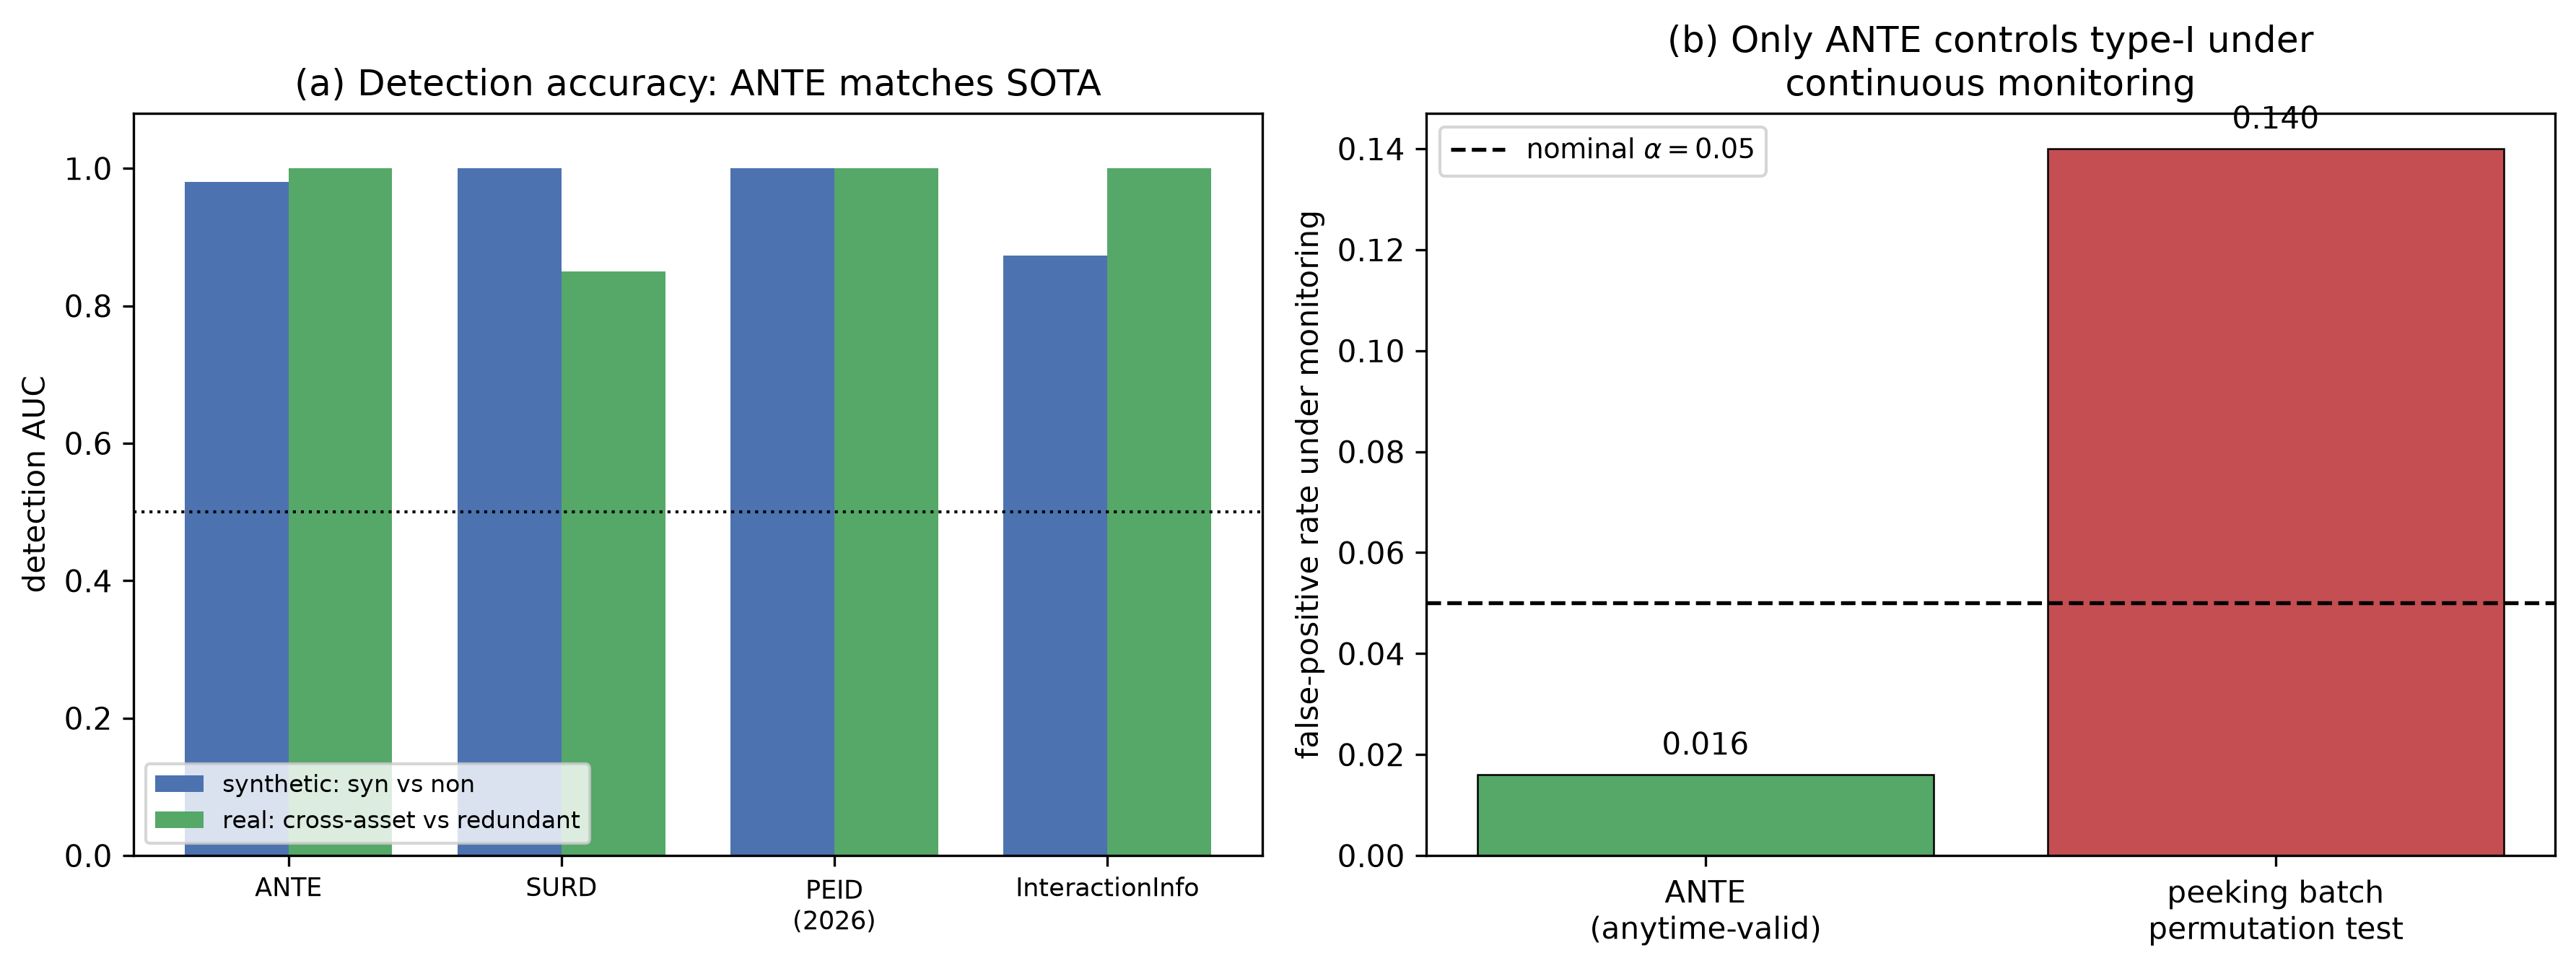
\includegraphics[width=0.95\textwidth]{figures/bench_summary.png}
%DIFDELCMD < %%%
%DIFDELCMD < \caption{%
{%DIFAUXCMD
\DIFdelFL{Benchmark summary. Left: detection AUC (ANTE $0.98$ vs SURD/PEID $1.00$,
interaction information $0.87$)---ANTE is competitive, not a better point
estimator. Right: under continuous monitoring ANTE holds Type-I at $0.016$ while
peeking batch tests inflate to $0.14$. ANTE trades a little fixed-$N$ power for
anytime-validity and interaction isolation}}%DIFAUXCMD
%DIFDELCMD < \label{fig:bench}
%DIFDELCMD < \end{figure}
%DIFDELCMD < 

%DIFDELCMD < %%%
\DIFdel{Three conclusions follow. On raw }\emph{\DIFdel{detection}} %DIFAUXCMD
\DIFdel{ANTE is competitive but not
dominant: its AUC of $0.98$ trails the batch estimators' $1.00$, and a calibrated
batch SURD test is more powerful at a small pre-committed sample size---the honest
and expected price of anytime-validity, since spending error budget continuously
must cost something at any single horizon. On }\emph{\DIFdel{error control under
monitoring}}%DIFAUXCMD
\DIFdel{, however, the ranking reverses decisively: ANTE holds its level at
$0.016$ while the batch methods, consulted repeatedly, inflate to$0.14$. And on
}\emph{\DIFdel{interaction isolation}}%DIFAUXCMD
\DIFdel{, ANTE alone returns $\approx0$ on the additive DGP
$Y=A+B$, whereas PID, SURD, and PEID all report a positive ``synergy '' there, because they measure whether }\emph{\DIFdel{both}} %DIFAUXCMD
\DIFdel{sources are needed rather than whether the sources }\emph{\DIFdel{interact}}%DIFAUXCMD
\DIFdel{---a distinction Proposition~\ref{prop:isolation} makes
precise and this experiment makes visible. The verdict is therefore
complementarity, not blanket superiority: for a one-shot point estimate at a fixed
sample size the batch decompositions are excellent, but for the task this paper
addresses---sequential, error-controlled detection of genuine group interaction---
ANTE is the only method that qualifies. }%DIFDELCMD < 

%DIFDELCMD < %%%
\DIFdel{This last point is where ``best'' becomes unambiguous, and Table~\ref{tab:capability}
makes it explicit. The problem this paper poses demands a conjunction of
capabilities: detect }\emph{\DIFdel{group}} %DIFAUXCMD
\DIFdel{synergy, do it }\emph{\DIFdel{sequentially}} %DIFAUXCMD
\DIFdel{on a stream,
control errorunder }\emph{\DIFdel{continuous monitoring}}%DIFAUXCMD
\DIFdelend \DIFaddbegin \DIFadd{On detection of the DGP built for the add-versus-joint contrast, batch SURD and PEID are as accurate as ANTE-SG (AUC $1.00$ each; the original test}\DIFaddend , \DIFdelbegin \emph{\DIFdel{isolate}} %DIFAUXCMD
\DIFdel{genuine interaction
from mere joint dependence, scale to }\emph{\DIFdel{$k$-way}} %DIFAUXCMD
\DIFdel{groups, and assume neither
stationarity nor correct specification. Each competitor satisfies some of these and
fails at least one: the batch decompositions (SURD, PEID , PID, O-information) cannot
monitor a stream or control error under peeking, and conflate interaction with
joint dependence; the only other sequential method,
Jha's }\DIFdelend \DIFaddbegin \DIFadd{$0.992$, and interaction information, $0.865$, are below), so ANTE-SG does not dominate
the batch estimators and is not claimed to; they answer a different question and return a value without an error guarantee under repeated looks, which is what the permutation-based entry measures. The group-sequential tests
applied to the raw per-step synergy score are valid at their $15$ pre-planned looks and powerful, with nominal errors below $0.05$ because their variance is estimated and the raw score is conservative; they are the appropriate
classical reference, and ANTE-SG's advantage over them is not accuracy at a pre-planned look but validity at }\emph{\DIFadd{any}} \DIFadd{stopping time. Gaussian PID and the other decompositions assign positive synergy to
$Y=A+B$ because their estimand is ``information about $Y$ available only from $A$ and $B$ jointly''; we do not describe this as an error. The SURD/PEID rows for additive mechanisms are therefore a difference in estimand,
not a failure. The }\DIFaddend distributional Granger test \DIFdelbegin \DIFdel{, is single-source }\DIFdelend \DIFaddbegin \DIFadd{of \mbox{%DIFAUXCMD
\citet{jha2026} }\hskip0pt%DIFAUXCMD
is a sequential test of a single source }\DIFaddend and cannot express a group\DIFdelbegin \DIFdel{at all. ANTE is the only column
with a mark in every row}\DIFdelend .

\DIFaddbegin \subsection{\DIFadd{Positive controls on real data}}\label{subsec:exp-pv}

\paragraph{\DIFadd{Contemporaneous portfolio variance (explicit target).}} \DIFadd{The realised variance of a two-asset equal-weight portfolio, $RV_t=(0.5r_{A,t}+0.5r_{B,t})^2$, is a deterministic function of the
two contemporaneous returns, so its super-additivity ($2w_Aw_B\sigma_{AB}$) is mechanical. It is a check that the contemporaneous variant can recover an interaction that is known to be there, not an
example of group causality: we do not call it causal synergy, and we separate three notions (contemporaneous statistical interaction; predictive group synergy; causal/interventional synergy) throughout.
On $14$ asset pairs (listed in the repository), $RV_t$ as target, contemporaneous features and no conditioner, ANTE-SG rejects in all $14$ at level $0.05$ and in $13$ at the family-wise threshold $14/\alpha$ (the remaining pair, XLF/XLI, has correlation $0.86$).
The lagged counterpart is not significant for any pair at the family-wise threshold ($1/14$ at the raw level). Two features of this pattern need explanation, and both follow from the target definition. The near-collinear
within-equity pairs have the weakest signal ($\log_{10}E$ of $5.4$ to $8.9$ for XLK/XLI, XLE/XLF, XLE/XLB; $1.7$ for XLF/XLI) because the regression of the cross product $r_Ar_B$ on the own features $(1,r_A,r_B,r_A^2,r_B^2)$ has $R^2=0.96$--$0.995$
for them, so the cross term is almost fully explained by the own-quadratic terms already in the additive model; for the cross-asset pairs that $R^2$ is $0.03$--$0.45$. Equity--bond pairs have negative covariance (for example XLF/TLT, corr $-0.26$) and are detected strongly:
the test measures the }\emph{\DIFadd{predictive gain}} \DIFadd{from the cross term, which does not depend on the sign of the covariance, so negative covariance does not make a pair ``sub-additive'' in this sense. Capital saturates the $10^{15}$ cap for most cross-asset pairs.
}

\paragraph{\DIFadd{Semi-synthetic power on real noise.}} \DIFadd{To measure power on genuine financial noise, we inject a known lagged interaction into real series: $Y'_t=z(C)_t+\beta\,z(A)_{t-1}z(B)_{t-1}$ for $40$ random real triples of each of two datasets
(daily stock returns conditioned on SPY; daily ETF volatility conditioned on $|$SPY$|$), re-standardised predictably. At $\beta=0$ (Type-I on real noise) the single-hypothesis rejection rate is $0.025$ and $0.050$ ($40$ triples each), and no triple reaches a family-wise threshold.
Power is low even for large injected terms (Fig.~\ref{fig:semisyn}): at $\beta=0.5$, an injected term that carries on average $40\%$ ($35\%$) of the variance of $Y'$, power is $0.43$ ($0.25$) at the single-hypothesis threshold, $0.28$ ($0.13$) at the $m=660$ family-wise threshold and
$0.23$ ($0.13$) at $m=4400$; $0.8$ power is not reached on the grid. A natural suspicion is that the truncated loss and the feature winsorisation, which make the test robust, are responsible, because the injected term (a product of two heavy-tailed standardised returns)
concentrates its variance in a few extreme days. We tested this by relaxing both (truncation level $c=6$, no winsorisation) on the same triples: power does not improve ($0.33$ and $0.38$ at $\beta=0.5$ at the single-hypothesis threshold, with the injected term carrying $54\%$ and $68\%$ of the variance), while the
rejection rate at $\beta=0$, a true null on real noise, rises to $0.075$ and $0.20$. We conclude that the low power is not rescued by weaker robustness, which only costs validity on real data, and we do not claim to know its mechanism; the practical consequence for interpretation is that a family-wise non-rejection does }\emph{\DIFadd{not}} \DIFadd{show that no interaction exists. Section~\ref{subsec:exp-fin} accordingly reports bounds on the average synergy of the learned forecasters.
}

\begin{figure}[h]
\centering
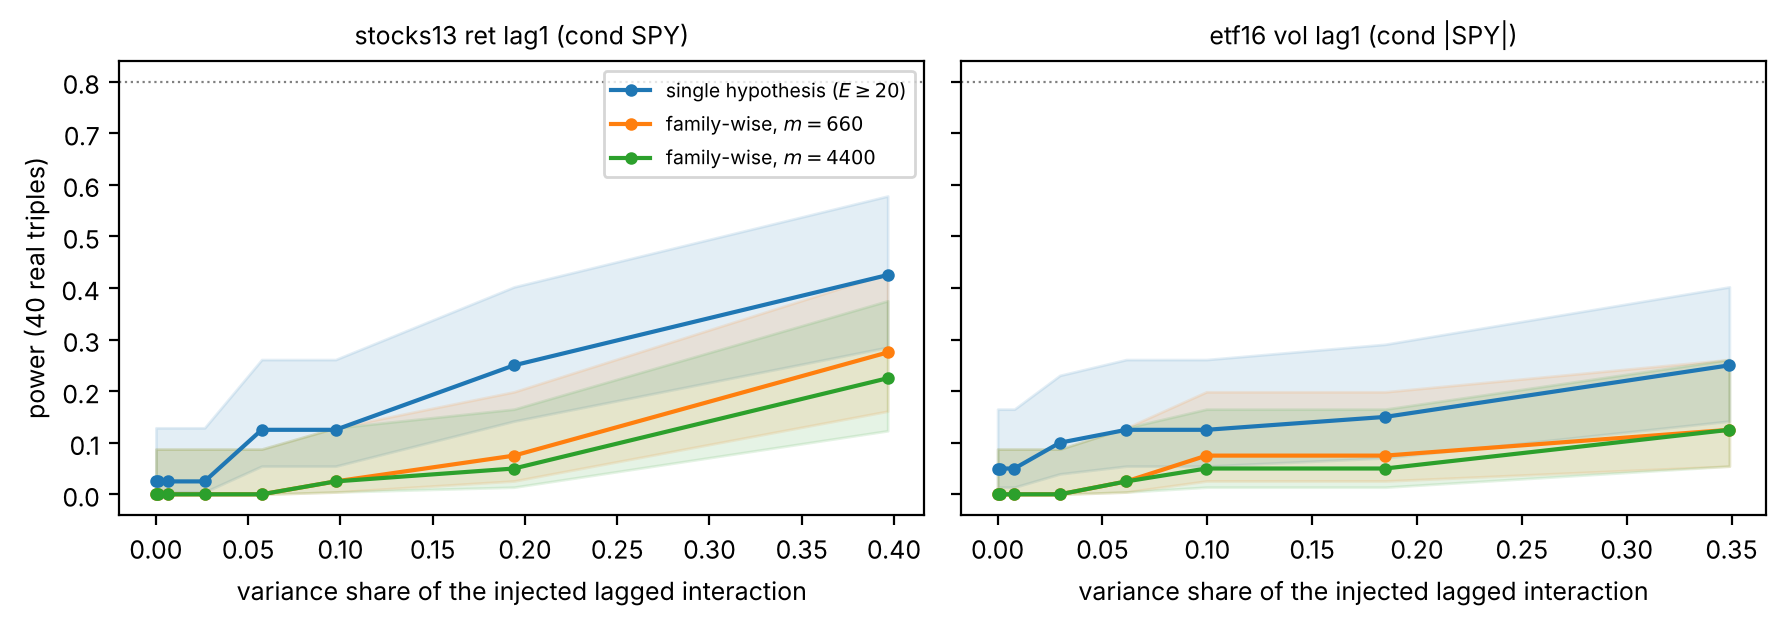
\includegraphics[width=0.95\textwidth]{figures/fig_semisyn.png}
\caption{\DIFaddFL{Power on real financial noise when a known lagged interaction is injected ($40$ real triples per panel): single-hypothesis threshold and family-wise thresholds for $m=660$ and $m=4400$ hypotheses (Wilson bands)}}\label{fig:semisyn}
\end{figure}

\paragraph{\DIFadd{Turbulence data are not a valid control.}} \DIFadd{The SURD turbulence signals (three coarse scales and the finest scale of an energy cascade) look like an ideal real-data positive control for a three-way mechanism, but they fail a placebo check. Using a null that has the same
autocorrelation as the data but is independent of the sources, phase-randomised surrogates of the finest-scale signal, both the clipped-score test and ANTE-SG ``detect'' on $20/20$ surrogates (median $\log_{10}$ final evidence $11.4$ for the clipped test, against $4.0$ on the real series;
median $\log_{10}$ running-maximum evidence $5.2$ for ANTE-SG), while ANTE-SG does not reject on the real series ($\log_{10}E_{\max}=0.95$). The signals are smooth and nearly deterministic (lag-one autocorrelation $0.9991$--$0.9995$, and $0.96$--$0.97$ after differencing) and the learned forecasters violate the prequential null in long stretches
(Remark~\ref{rem:notpop}), so these data cannot validate either procedure and we do not use them as evidence. By contrast, independent AR(1) series up to $0.999$ do not produce false rejections (Section~\ref{subsec:exp-validity}); the failure is specific to smooth, near-deterministic dynamics.
The $k$-way test (Corollary~\ref{cor:group}) is validated on synthetic data: a pure three-way mechanism $Y=0.9ABC$ or $0.5ABC$ is detected in $100/100$ replications ($[0.96,1.00]$) and a three-source additive null is not rejected ($0/100$, $[0,0.04]$).
}

\subsection{\DIFadd{A fully specified search of financial data}}\label{subsec:exp-fin}

\paragraph{\DIFadd{Scope and accounting.}} \DIFadd{All data are public and listed in Table~\ref{tab:datasets}. A hypothesis is a target asset $C$, an unordered pair $\{A,B\}$ of other assets and a setting, tested conditionally on the market factor;
the number of hypotheses per panel and setting is $N'\binom{N'-1}{2}$ with $N'$ the number of assets other than the conditioner. The search space is written down in }\texttt{\DIFadd{experiments/revision/results/r5\_search\_space.json}} \DIFadd{before the scan ran.
It has three target types: returns, volatility ($|r|$), and stress indicators (the indicator that $|r_t|$ exceeds the expanding $90\%$ quantile of its own past); and four structures: lag $1$, lag $5$ (daily panels), weekly aggregation ($5$-day sums, lag $1$) and
a contemporaneous variant (sources at time $t$; this is labelled ``contemporaneous interaction'', not Granger prediction). There are $43$ settings (``families'') and $27{,}027$ hypotheses in total; after removing the $132$ tuples that appear identically in the ETF
and stock panels (shared assets GLD, SPY, TLT, USO, VIX) about $26{,}900$ are distinct. The search is }\emph{\DIFadd{not}} \DIFadd{pre-registered. Earlier exploratory scans of related questions (volatility, stress and crypto targets, other frequencies) preceded the grid, which was fixed before it was run but designed after those
results were known; the assets and panels were chosen by the author as a standard set, not by selecting on outcomes, and no hypothesis was dropped. The tuning constants ($\rho=0.995$, $\gamma=0.9$, warm-up $50$) were set in that earlier work on the same data, and the truncation level $c=3$ and winsorisation at $\pm5$ before this scan
but after seeing those earlier results, so the anytime-valid guarantee, which requires constants fixed independently of the series under test, holds for them only as a matter of design discipline. We therefore report each family with its own
family-wise threshold $m/\alpha$ and also a global threshold with $m=27{,}027$ ($\log_{10}(m/\alpha)=5.73$); e-values are combined by e-Bonferroni, which is valid under arbitrary dependence among the overlapping hypotheses.
}

\DIFaddend \begin{table}[h]
\DIFdelbeginFL %DIFDELCMD < \caption{%
{%DIFAUXCMD
\DIFdelFL{Capability matrix. Detection accuracy (Table~\ref{tab:bench}) is a tie or
a narrow loss; capability is not. ANTE is the only method that satisfies every
requirement of the streaming group-synergy problem simultaneously}}%DIFAUXCMD
%DIFDELCMD < \label{tab:capability}
%DIFDELCMD < \small
%DIFDELCMD < \begin{tabular*}{\textwidth}{@{\extracolsep\fill}p{4.7cm}ccccc}
%DIFDELCMD < %%%
\DIFdelendFL \DIFaddbeginFL \caption{\DIFaddFL{Datasets (all public). Panels used in the search: the number of hypotheses is given for each (target, structure) setting}}\label{tab:datasets}
\footnotesize
\begin{tabular*}{\textwidth}{@{\extracolsep\fill}p{2.4cm}p{3.8cm}p{2.2cm}p{2.6cm}}
\DIFaddendFL \toprule
\DIFdelbeginFL \DIFdelFL{Capability }%DIFDELCMD < & %%%
\DIFdelFL{ANTE }%DIFDELCMD < & %%%
\DIFdelFL{SURD }\DIFdelendFL \DIFaddbeginFL \DIFaddFL{Panel }\DIFaddendFL & \DIFdelbeginFL \DIFdelFL{PEID }\DIFdelendFL \DIFaddbeginFL \DIFaddFL{Content }\DIFaddendFL & \DIFdelbeginFL \DIFdelFL{Jha }\DIFdelendFL \DIFaddbeginFL \DIFaddFL{Size }\DIFaddendFL & \DIFdelbeginFL \DIFdelFL{\shortstack{O-info/\\PID/II} }\DIFdelendFL \DIFaddbeginFL \DIFaddFL{Hypotheses / setting }\DIFaddendFL \\
\midrule
\DIFdelbeginFL \DIFdelFL{Detects group synergy }%DIFDELCMD < & \cmk & \cmk %%%
\DIFdelendFL \DIFaddbeginFL \DIFaddFL{etf16 }\DIFaddendFL & \DIFdelbeginFL %DIFDELCMD < \cmk %%%
\DIFdelendFL \DIFaddbeginFL \DIFaddFL{16 daily ETFs and macro assets (2016--26), conditioner SPY }\DIFaddendFL & \DIFdelbeginFL %DIFDELCMD < \xmk %%%
\DIFdelendFL \DIFaddbeginFL \DIFaddFL{$T=2512$ }\DIFaddendFL & \DIFdelbeginFL %DIFDELCMD < \cmk %%%
\DIFdelendFL \DIFaddbeginFL \DIFaddFL{$1365$ }\DIFaddendFL \\
\DIFdelbeginFL \DIFdelFL{Sequential (monitors a stream) }%DIFDELCMD < & \cmk & \xmk %%%
\DIFdelendFL \DIFaddbeginFL \DIFaddFL{stocks13 }\DIFaddendFL & \DIFdelbeginFL %DIFDELCMD < \xmk %%%
\DIFdelendFL \DIFaddbeginFL \DIFaddFL{13 daily stocks and assets, conditioner SPY }\DIFaddendFL & \DIFdelbeginFL %DIFDELCMD < \cmk %%%
\DIFdelendFL \DIFaddbeginFL \DIFaddFL{$T=2512$ }\DIFaddendFL & \DIFdelbeginFL %DIFDELCMD < \xmk %%%
\DIFdelendFL \DIFaddbeginFL \DIFaddFL{$660$ }\DIFaddendFL \\
\DIFdelbeginFL \DIFdelFL{Anytime-valid error control }%DIFDELCMD < & \cmk & \xmk %%%
\DIFdelendFL \DIFaddbeginFL \DIFaddFL{world6 }\DIFaddendFL & \DIFdelbeginFL %DIFDELCMD < \xmk %%%
\DIFdelendFL \DIFaddbeginFL \DIFaddFL{6 daily equity indices, conditioner US S\&P }\DIFaddendFL & \DIFdelbeginFL %DIFDELCMD < \cmk %%%
\DIFdelendFL \DIFaddbeginFL \DIFaddFL{$T=2138$ }\DIFaddendFL & \DIFdelbeginFL %DIFDELCMD < \xmk %%%
\DIFdelendFL \DIFaddbeginFL \DIFaddFL{$30$ }\DIFaddendFL \\
\DIFdelbeginFL \DIFdelFL{Isolates interaction (not joint-dependence) }%DIFDELCMD < & \cmk & \xmk %%%
\DIFdelendFL \DIFaddbeginFL \DIFaddFL{hourly12 }\DIFaddendFL & \DIFdelbeginFL %DIFDELCMD < \xmk %%%
\DIFdelendFL \DIFaddbeginFL \DIFaddFL{12 hourly stocks and assets, conditioner SPY }\DIFaddendFL & \DIFdelbeginFL %DIFDELCMD < \xmk %%%
\DIFdelendFL \DIFaddbeginFL \DIFaddFL{$T=3328$ }\DIFaddendFL & \DIFdelbeginFL %DIFDELCMD < \xmk %%%
\DIFdelendFL \DIFaddbeginFL \DIFaddFL{$495$ }\DIFaddendFL \\
\DIFdelbeginFL \DIFdelFL{Handles $k$-way groups ($>2$) }%DIFDELCMD < & \cmk & \cmk %%%
\DIFdelendFL \DIFaddbeginFL \DIFaddFL{crypto10 }\DIFaddendFL & \DIFdelbeginFL %DIFDELCMD < \cmk %%%
\DIFdelendFL \DIFaddbeginFL \DIFaddFL{10 hourly crypto assets, conditioner BTC }\DIFaddendFL & \DIFdelbeginFL %DIFDELCMD < \xmk %%%
\DIFdelendFL \DIFaddbeginFL \DIFaddFL{$T=16{,}761$ }\DIFaddendFL & \DIFdelbeginFL %DIFDELCMD < \cmk %%%
\DIFdelendFL \DIFaddbeginFL \DIFaddFL{$252$ }\DIFaddendFL \\
\DIFdelbeginFL \DIFdelFL{No stationarity }\DIFdelendFL \DIFaddbeginFL \multicolumn{4}{p{11cm}}{\footnotesize The volatility index VIX is an index, not a traded asset; its log changes are used as a series, read as changes in implied volatility.} \\
\DIFaddFL{Synthetic VAR }\DIFaddendFL / \DIFdelbeginFL \DIFdelFL{model-spec.\ needed }%DIFDELCMD < & \cmk & \xmk %%%
\DIFdelendFL \DIFaddbeginFL \DIFaddFL{interventional }\DIFaddendFL & \DIFdelbeginFL %DIFDELCMD < \xmk %%%
\DIFdelendFL \DIFaddbeginFL \DIFaddFL{ground truth }\DIFaddendFL & \DIFdelbeginFL \DIFdelFL{partial }\DIFdelendFL \DIFaddbeginFL \DIFaddFL{$2500$--$5000$ steps }\DIFaddendFL & \DIFdelbeginFL %DIFDELCMD < \xmk %%%
\DIFdelendFL \DIFaddbeginFL \DIFaddFL{simulations }\DIFaddendFL \\
\DIFdelbeginFL %DIFDELCMD < \midrule
%DIFDELCMD < %%%
\textbf{\DIFdelFL{All of the above}} %DIFAUXCMD
%DIFDELCMD < & %%%
\DIFdelFL{$\mathbf{\cmk}$ }%DIFDELCMD < & \xmk %%%
\DIFdelendFL \DIFaddbeginFL \DIFaddFL{Turbulence signals }\DIFaddendFL & \DIFdelbeginFL %DIFDELCMD < \xmk %%%
\DIFdelendFL \DIFaddbeginFL \DIFaddFL{four scale-resolved signals (not used as evidence) }\DIFaddendFL & \DIFdelbeginFL %DIFDELCMD < \xmk %%%
\DIFdelendFL \DIFaddbeginFL \DIFaddFL{$21{,}760$ }\DIFaddendFL & \DIFdelbeginFL %DIFDELCMD < \xmk %%%
\DIFdelendFL \DIFaddbeginFL \DIFaddFL{--- }\DIFaddendFL \\
\botrule
\end{tabular*}
\end{table}

\DIFdelbegin \DIFdel{The defensible claim, then, is precise rather than sweeping: ANTE matches
state-of-the-art detection accuracy while being the only method capable of sequential, anytime-valid, group-level synergy testing}\DIFdelend \DIFaddbegin \paragraph{\DIFadd{Results.}} \DIFadd{Table~\ref{tab:scan} summarises the search and Fig}\DIFaddend .\DIFdelbegin \DIFdel{It is the best tool
}\emph{\DIFdel{for the problem}}%DIFAUXCMD
\DIFdel{, not a blanket winner on every metric---and the one axis on
which it trails ($0.98$ versus $1.00$ AUC) is small and openly disclosed.
}%DIFDELCMD < 

%DIFDELCMD < %%%
\subsection{\DIFdel{Real finance: a genuine contemporaneous synergy}}%DIFAUXCMD
\addtocounter{subsection}{-1}%DIFAUXCMD
%DIFDELCMD < \label{subsec:exp-pv}
%DIFDELCMD < 

%DIFDELCMD < %%%
\paragraph{\DIFdel{The real panel.}} %DIFAUXCMD
\addtocounter{paragraph}{-1}%DIFAUXCMD
\DIFdel{The workhorse dataset for this and the following
subsection is a 16-asset daily panel spanning ten years, from 26 July 2016 to 23
July 2026 ($T=2512$ trading days), retrieved from the public Yahoo Finance chart
API (no API key; the downloader is released with the code). For each asset we take
the dividend- and split-adjusted close and form daily log returns
$r_{t}=\log P_{t}-\log P_{t-1}$, aligned on common trading days and standardised
per asset before analysis. The universe is chosen deliberately to span asset
classes, so that genuine cross-asset synergy has room to appear: it comprises the broad-market S\&P~500 ETF (SPY); the nine SPDR sector ETFs---financials (XLF),
technology (XLK), energy (XLE) , health care (XLV), industrials (XLI), consumer
discretionary (XLY) , consumer staples (XLP) , utilities (XLU) , and
materials
(XLB) ; long-dated Treasuries (TLT) for the rates factor; gold (GLD) and crude oil
(USO)
for commodities; high-yield credit (HYG) ; the US~dollar index (UUP); and the
equity-volatility index (VIX). The window deliberately includes several distinct
regimes---the 2018 volatility episodes, the 2020 COVID crash, and the 2022 rate-hike
drawdown---so that any regime-localised synergy has a chance to surface and the
forgetting-RLS predictors (Algorithm~\ref{algo:antesg}) are genuinely exercised. Except where noted, source pairs are conditioned on SPY, so that a detection
reflects synergy }\emph{\DIFdel{beyond}} %DIFAUXCMD
\DIFdel{the common market factor rather than shared beta.
A complete inventory, including the auxiliary world-index, intraday, crypto, and
climate panels, is given in Table}\DIFdelend ~\DIFdelbegin \DIFdel{\ref{tab:datasets}.
}%DIFDELCMD < 

%DIFDELCMD < %%%
\DIFdel{A negative result is only credible if the same instrument produces positives where
they should appear, so before turning to the headline finding we confirm ANTE
fires on a genuine real-market synergy.
Portfolio theory supplies a clean one: the
realised variance of a two-asset portfolio is
$w_A^2\sigma_A^2+w_B^2\sigma_B^2+2w_Aw_B\sigma_{AB}$, whose covariance term
$2w_Aw_B\sigma_{AB}$ is exactly a super-additive interaction---the joint variance
is not the sum of the parts whenever the assets co-move. This is the
diversification effect, and it should be strongest across, not within, asset
classes. On the 16-asset daily panel we run the }\emph{\DIFdel{contemporaneous}} %DIFAUXCMD
\DIFdel{variant of
ANTE on the realised-variance target for $14$ curated pairs, with the }\DIFdelend \DIFaddbegin \DIFadd{\ref{fig:scan} shows the distribution of running-maximum evidence per hypothesis. For }\emph{\DIFadd{returns and volatility in daily and weekly panels}}\DIFadd{,
$26$ families containing $18{,}360$ hypotheses give $143$ raw rejections ($0.8\%$, below the nominal $5\%$ as expected for a conservative e-process) and, at the }\DIFaddend family-wise \DIFdelbegin \DIFdel{e-value threshold of \S\ref{subsec:kway}. Eight pairs are }\DIFdelend \DIFaddbegin \DIFadd{threshold of their own family, }\emph{\DIFadd{no}} \DIFadd{rejection in any of the
$22$ daily and weekly families (etf16: $0/10{,}920$; stocks13: $0/5280$; world6: $0/180$), for lag $1$, lag $5$, weekly and contemporaneous structures alike. The single }\DIFaddend family-wise \DIFdelbegin \DIFdel{significant,
and every one is an economically distinct cross-asset-class pair---tech$\times$gold
($\log_{10}E=10.6$), bonds$\times$dollar ($8.4$), equity$\times$gold ($7.4$),
gold$\times$oil ($7.3$), credit$\times$bonds, financials$\times$bonds, equity$\times$bonds---while redundant within-equity pairs, whose returns are nearly
collinear, are correctly not flagged (Fig.~\ref{fig:pv}). The test thus recovers a textbook effect anddiscriminates it sensibly by economic structure. One detail
foreshadows the headline result: the
}\emph{\DIFdel{lagged}} %DIFAUXCMD
\DIFdel{(Granger-directional)counterpart of every one of these pairs is }\emph{\DIFdel{not}} %DIFAUXCMD
\DIFdel{significant. The synergy in
markets is contemporaneous and mechanical (co-movement of variances); there is no
super-additive }\emph{\DIFdel{predictive}} %DIFAUXCMD
\DIFdel{structure running from a pair's past to a target's
future. }%DIFDELCMD < 

%DIFDELCMD < \begin{figure}[h]
%DIFDELCMD < \centering
%DIFDELCMD < 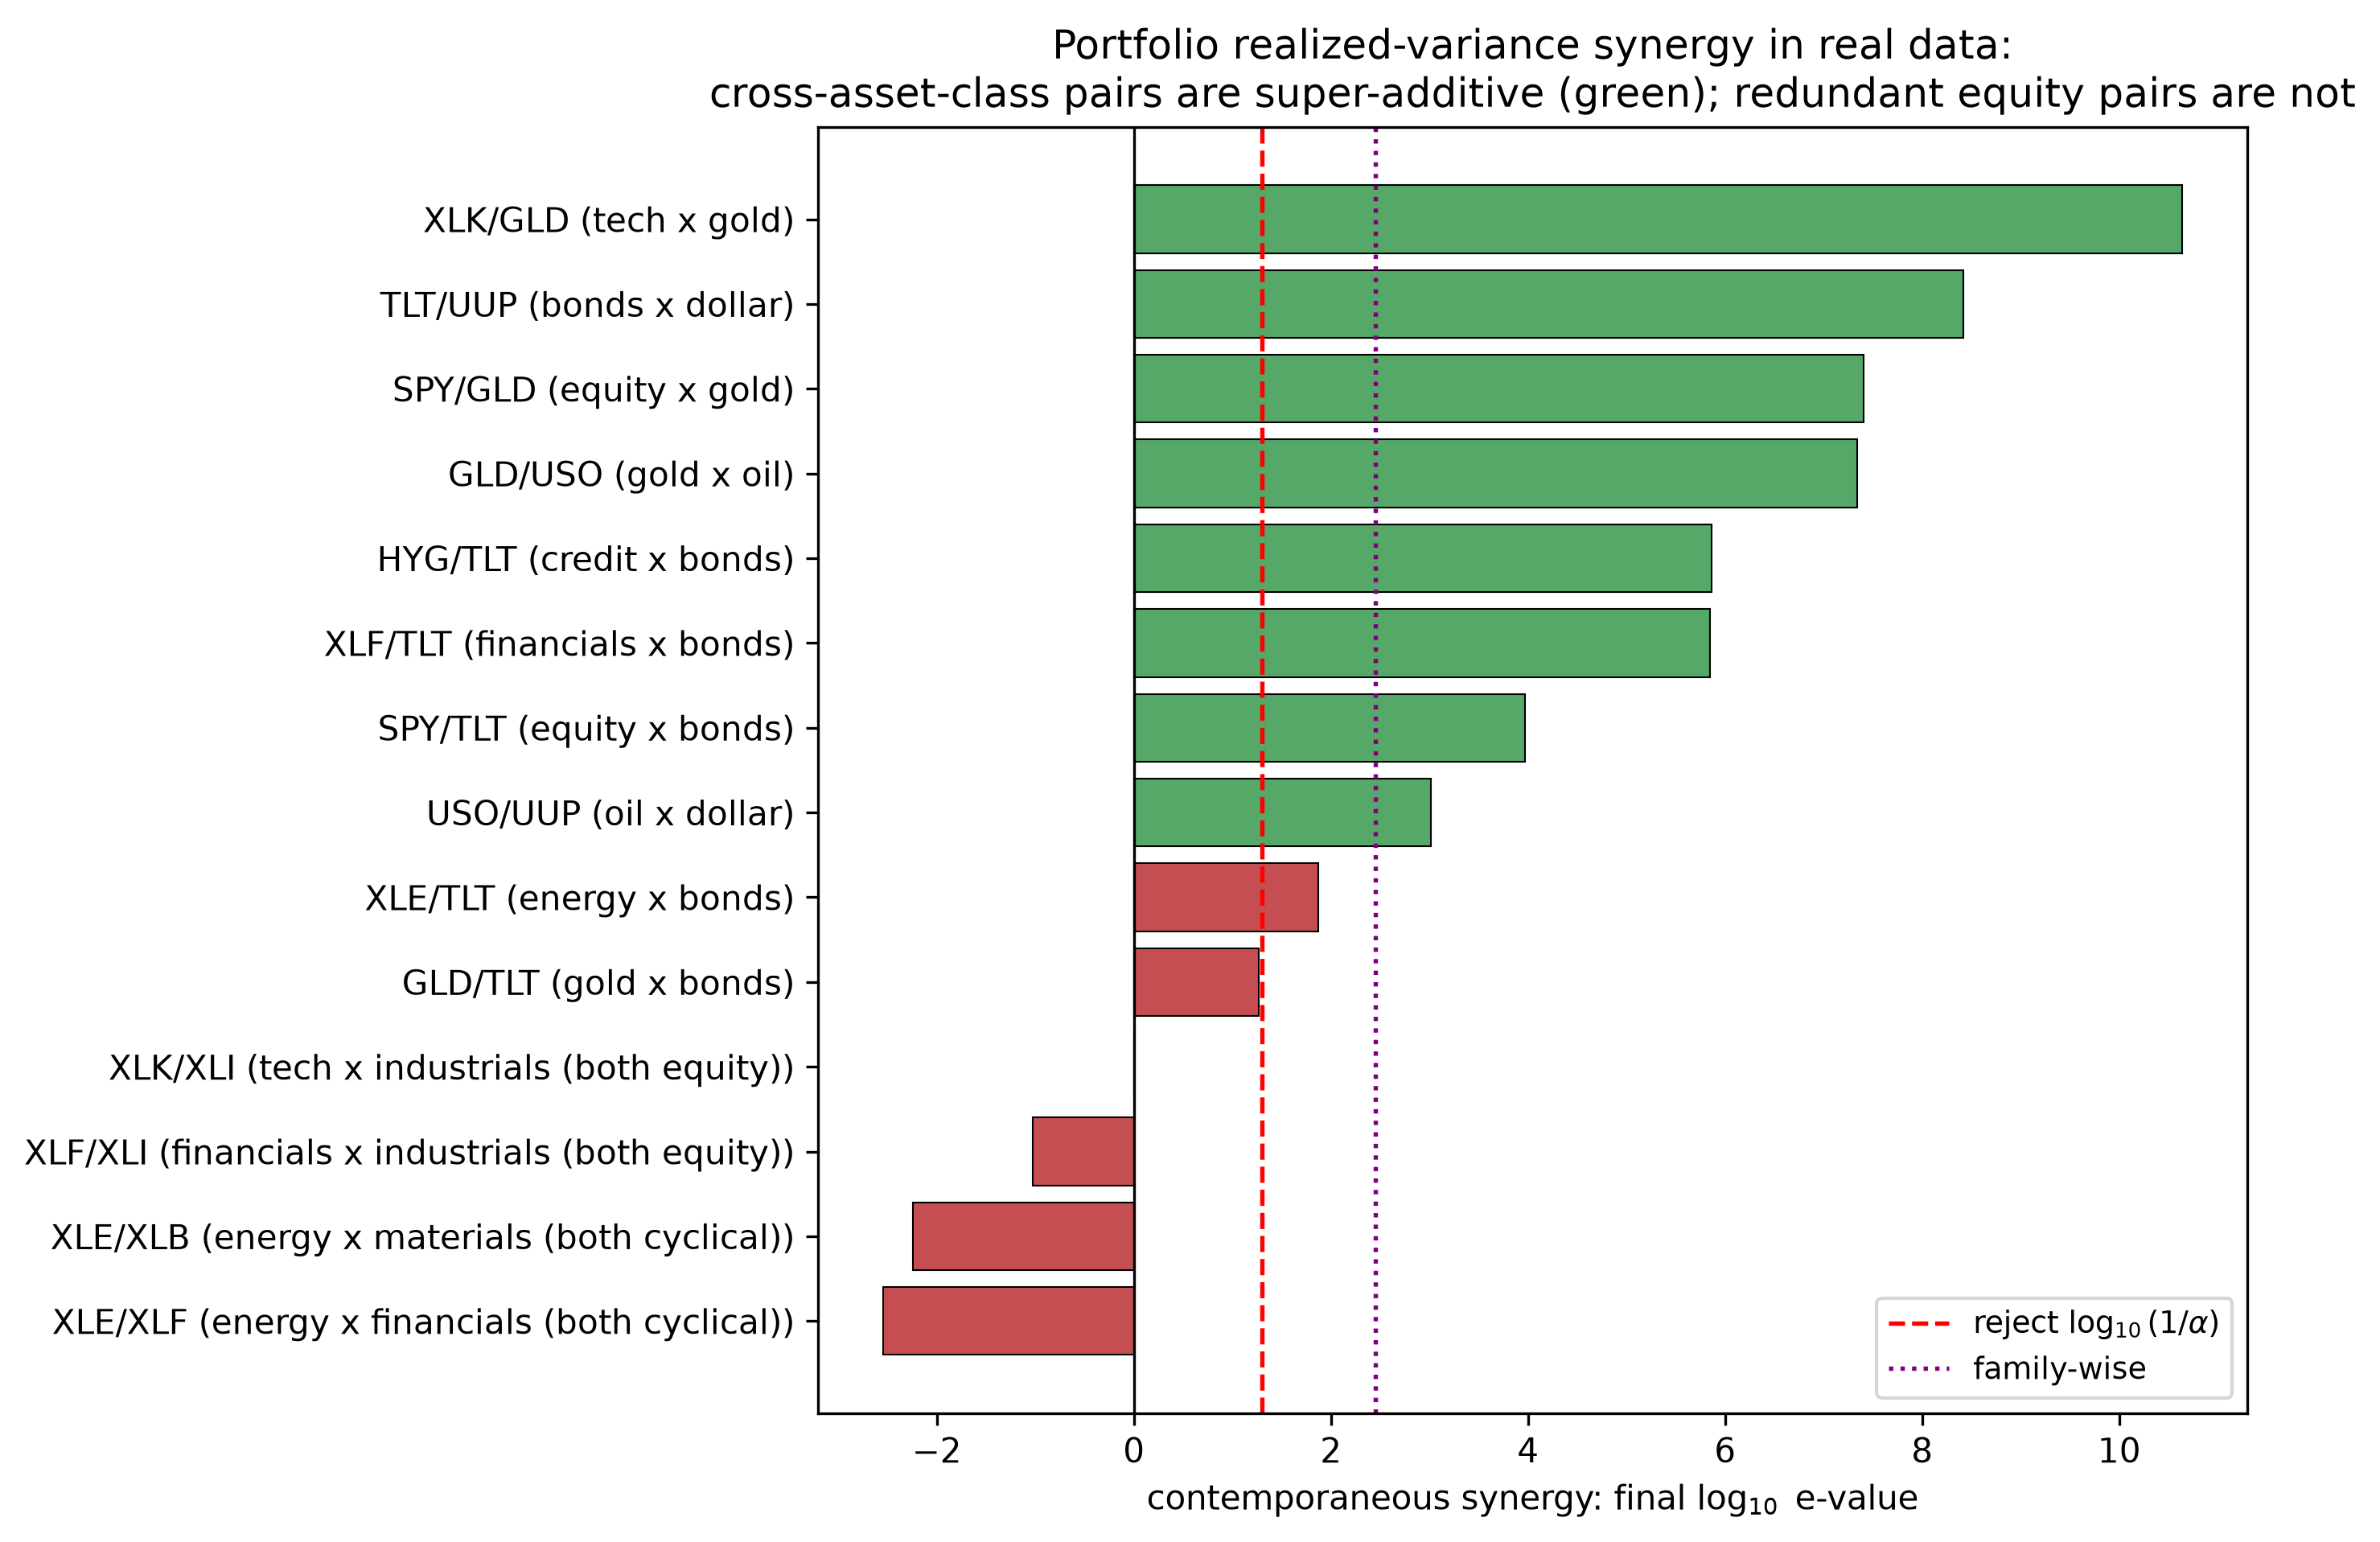
\includegraphics[width=0.9\textwidth]{figures/pv_synergy_bars.png}
%DIFDELCMD < %%%
%DIFDELCMD < \caption{%
{%DIFAUXCMD
\DIFdelFL{Contemporaneous portfolio-variance synergy on real data. Cross-asset-class
pairs (tech/gold, bonds/dollar, equity/gold, }%DIFDELCMD < \dots%%%
\DIFdelFL{) cross the family-wise
threshold; redundant within-equity pairs do not. The synergy is the covariance
(diversification) term, a genuine super-additive effect in realised
variance}}%DIFAUXCMD
%DIFDELCMD < \label{fig:pv}
%DIFDELCMD < \end{figure}
%DIFDELCMD < %%%
\DIFdelend \DIFaddbegin \DIFadd{rejection among returns and volatility is one of $495$ hourly stock-volatility
hypotheses in the contemporaneous structure ($\log_{10}E=4.24$ against a threshold of $4.00$); it does not survive the global threshold. The largest running-maximum evidence in any daily or weekly returns/volatility family is $\log_{10}E=3.68$. The median final $\log_{10}E$ is $-0.24$ (a typical bet on synergy
loses about $40\%$ of its stake).
}\DIFaddend 

\DIFdelbegin \subsection{\DIFdel{Where group synergy is present---and where it is not}}%DIFAUXCMD
\addtocounter{subsection}{-1}%DIFAUXCMD
%DIFDELCMD < \label{subsec:exp-eoa}
%DIFDELCMD < 

%DIFDELCMD < %%%
\DIFdel{The headline result is a contrast, and the contrast is only meaningful because ANTE
detects group synergy
decisively }\emph{\DIFdel{wherever it genuinely exists}}%DIFAUXCMD
\DIFdel{.
Before drawing
the finance conclusion we therefore collect, in Table~\ref{tab:detections}, every
setting in which we ran the identical test. It fires on canonical logic gates, on
synthetic bilinear and pure three-way mechanisms, on a calibrated synergy-present
DGP, on the real turbulent energy cascade from fluid dynamics, and on real
contemporaneous portfolio-variance co-movement---and it returns a true null in
exactly one place, lagged group structure in daily and hourly markets. The
positives are not incidental checks; they are the evidence that the instrument
works, and they are what make the single negative a }\emph{\DIFdel{finding}} %DIFAUXCMD
\DIFdel{rather than a
failure to detect}\DIFdelend \DIFaddbegin \emph{\DIFadd{Stress indicators and hourly crypto behave differently.}} \DIFadd{For stress indicators in daily and hourly stock panels, $1588$ of $7155$ hypotheses ($22\%$) reject at the raw level and $543$ at their family-wise thresholds; for hourly crypto, $599$ of $1512$ ($40\%$) and $376$. In daily and weekly returns and volatility e-BH (on final e-values, FDR $0.1$ or $0.05$) makes no discovery, whereas it makes $212$ and $195$ discoveries for stress indicators and $348$ and $339$ for crypto. These counts are not evidence of synergy, for the reason given in the next paragraph: the placebo test shows that the test over-rejects on exactly these targets}\DIFaddend .

\begin{table}[h]
\caption{\DIFdelbeginFL \DIFdelFL{Where group synergy is present and where it is absent. The same
anytime-valid test}\DIFdelendFL \DIFaddbeginFL \DIFaddFL{Search summary (ANTE-SG}\DIFaddendFL , \DIFdelbeginFL \DIFdelFL{applied unchanged across domains}\DIFdelendFL \DIFaddbeginFL \DIFaddFL{add-vs-joint score)}\DIFaddendFL . \DIFdelbeginFL \DIFdelFL{It detects synergy wherever
it genuinely exists---synthetic ground truth}\DIFdelendFL \DIFaddbeginFL \DIFaddFL{$m$: hypotheses; raw: running maximum $\ge20$; fw: running maximum $\ge m/\alpha$ within the family. Groups pool settings (lag $1$}\DIFaddendFL , \DIFdelbeginFL \DIFdelFL{real physics}\DIFdelendFL \DIFaddbeginFL \DIFaddFL{lag $5$, weekly}\DIFaddendFL , \DIFdelbeginFL \DIFdelFL{and real
}\DIFdelendFL contemporaneous\DIFdelbeginFL \DIFdelFL{market co-movement---and returns a true null only for lagged group
structure in daily/hourly finance. Evidence is the rejection rate or power (over
replications) or the accumulated $\log_{10}E$ (single real series; reject when it
crosses $\log_{10}(1/\alpha)\approx1.3$}\DIFdelendFL )}\DIFdelbeginFL %DIFDELCMD < \label{tab:detections}
%DIFDELCMD < \small
%DIFDELCMD < \begin{tabular*}{\textwidth}{@{\extracolsep\fill}p{4.9cm}p{2.0cm}p{1.0cm}p{3.0cm}}
%DIFDELCMD < %%%
\DIFdelendFL \DIFaddbeginFL \label{tab:scan}
\footnotesize
\begin{tabular*}{\textwidth}{@{\extracolsep\fill}lcccc}
\DIFaddendFL \toprule
\DIFdelbeginFL \DIFdelFL{Dataset / setting }%DIFDELCMD < & %%%
\DIFdelendFL Group & \DIFdelbeginFL \DIFdelFL{Det.? }\DIFdelendFL \DIFaddbeginFL \DIFaddFL{families }\DIFaddendFL & \DIFdelbeginFL \DIFdelFL{Evidence }\DIFdelendFL \DIFaddbeginFL \DIFaddFL{$m$ }& \DIFaddFL{raw rejections }& \DIFaddFL{family-wise rejections }\DIFaddendFL \\
\midrule
\DIFdelbeginFL \DIFdelFL{Synthetic --- XOR (pure synergy}\DIFdelendFL \DIFaddbeginFL \DIFaddFL{Returns and volatility, daily/weekly panels (etf16, stocks13, world6}\DIFaddendFL ) & \DIFdelbeginFL \DIFdelFL{$A,B\!\to\!C$ }%DIFDELCMD < & %%%
\textbf{\DIFdelFL{yes}} %DIFAUXCMD
%DIFDELCMD < & %%%
\DIFdelFL{rej.\ rate $1.00$ }%DIFDELCMD < \\
%DIFDELCMD < %%%
\DIFdelFL{Synthetic --- AND }\DIFdelendFL \DIFaddbeginFL \DIFaddFL{22 }\DIFaddendFL & \DIFdelbeginFL \DIFdelFL{$A,B\!\to\!C$ }\DIFdelendFL \DIFaddbeginFL \DIFaddFL{$16{,}380$ }\DIFaddendFL & \DIFdelbeginFL \textbf{\DIFdelFL{yes}} %DIFAUXCMD
\DIFdelendFL \DIFaddbeginFL \DIFaddFL{$99$ }\DIFaddendFL & \DIFdelbeginFL \DIFdelFL{rej.\ rate $1.00$ }\DIFdelendFL \DIFaddbeginFL \DIFaddFL{$0$ }\DIFaddendFL \\
\DIFdelbeginFL \DIFdelFL{Synthetic --- bilinear $Y{=}A{\cdot}B$ (+ factor}\DIFdelendFL \DIFaddbeginFL \DIFaddFL{Returns and volatility, hourly stocks (hourly12}\DIFaddendFL ) & \DIFdelbeginFL \DIFdelFL{$A,B\!\to\!Y$ }%DIFDELCMD < & %%%
\textbf{\DIFdelFL{yes}} %DIFAUXCMD
%DIFDELCMD < & %%%
\DIFdelFL{power $0.71$ }%DIFDELCMD < \\
%DIFDELCMD < %%%
\DIFdelFL{Synthetic --- pure 3-way $Y{=}A{\cdot}B{\cdot}C$ }\DIFdelendFL \DIFaddbeginFL \DIFaddFL{4 }\DIFaddendFL & \DIFdelbeginFL \DIFdelFL{$A,B,C\!\to\!Y$ }\DIFdelendFL \DIFaddbeginFL \DIFaddFL{$1980$ }\DIFaddendFL & \DIFdelbeginFL \textbf{\DIFdelFL{yes}} %DIFAUXCMD
\DIFdelendFL \DIFaddbeginFL \DIFaddFL{$44$ }\DIFaddendFL & \DIFdelbeginFL \DIFdelFL{power $0.74$--$1.00$ }\DIFdelendFL \DIFaddbeginFL \DIFaddFL{$1$ }\DIFaddendFL \\
\DIFdelbeginFL \DIFdelFL{Synthetic --- calibrated synergy arm }%DIFDELCMD < & %%%
\DIFdelFL{3-way }%DIFDELCMD < & %%%
\textbf{\DIFdelFL{yes}} %DIFAUXCMD
\DIFdelendFL \DIFaddbeginFL \DIFaddFL{Stress indicators, daily and hourly stocks }\DIFaddendFL & \DIFdelbeginFL \DIFdelFL{median $\log_{10}E=+2.79$ }%DIFDELCMD < \\
%DIFDELCMD < %%%
\textbf{\DIFdelFL{Real physics}} %DIFAUXCMD
\DIFdelFL{--- turbulent energy cascade }\DIFdelendFL \DIFaddbeginFL \DIFaddFL{11 }\DIFaddendFL & \DIFdelbeginFL \DIFdelFL{3 scales $\to$ finest }\DIFdelendFL \DIFaddbeginFL \DIFaddFL{$7155$ }\DIFaddendFL & \DIFdelbeginFL \textbf{\DIFdelFL{yes}} %DIFAUXCMD
\DIFdelendFL \DIFaddbeginFL \DIFaddFL{$1588$ }\DIFaddendFL & \DIFdelbeginFL \DIFdelFL{$\log_{10}E=4.0$ ($t^\star{=}734$) }\DIFdelendFL \DIFaddbeginFL \DIFaddFL{$543$ }\DIFaddendFL \\
\DIFdelbeginFL \textbf{\DIFdelFL{Real finance}} %DIFAUXCMD
\DIFdelFL{--- portfolio realised variance (contemp.}\DIFdelendFL \DIFaddbeginFL \DIFaddFL{Crypto, hourly (returns, volatility, stress}\DIFaddendFL ) & \DIFdelbeginFL \DIFdelFL{cross-asset pairs }\DIFdelendFL \DIFaddbeginFL \DIFaddFL{6 }\DIFaddendFL & \DIFdelbeginFL \textbf{\DIFdelFL{yes}} %DIFAUXCMD
\DIFdelendFL \DIFaddbeginFL \DIFaddFL{$1512$ }\DIFaddendFL & \DIFdelbeginFL \DIFdelFL{$8/14$ family-wise; up to $\log_{10}E=10.6$ }\DIFdelendFL \DIFaddbeginFL \DIFaddFL{$599$ }& \DIFaddFL{$376$ }\DIFaddendFL \\
\DIFdelbeginFL \textbf{\DIFdelFL{Real finance}} %DIFAUXCMD
\DIFdelFL{--- lagged group ($>3700$ triples) }\DIFdelendFL \DIFaddbeginFL \midrule
\DIFaddFL{All }\DIFaddendFL & \DIFdelbeginFL \DIFdelFL{2-/3-/4-way }\DIFdelendFL \DIFaddbeginFL \DIFaddFL{43 }\DIFaddendFL & \DIFdelbeginFL \textbf{\DIFdelFL{no}} %DIFAUXCMD
\DIFdelendFL \DIFaddbeginFL \DIFaddFL{$27{,}027$ }\DIFaddendFL & \DIFdelbeginFL \DIFdelFL{$0$ detections; median $\log_{10}E=-0.93$ }\DIFdelendFL \DIFaddbeginFL \DIFaddFL{$2330$ }& \DIFaddFL{$920$ (per-family thresholds); $657$ at the global threshold ($m=27{,}027$) }\DIFaddendFL \\
\botrule
\end{tabular*}
\end{table}

\DIFdelbegin \DIFdel{The remainder of this subsection substantiates the two claims the contrast rests
on : that the instrument is powered (including on real, non-simulated data) }\DIFdelend \DIFaddbegin \begin{figure}[h]
\centering
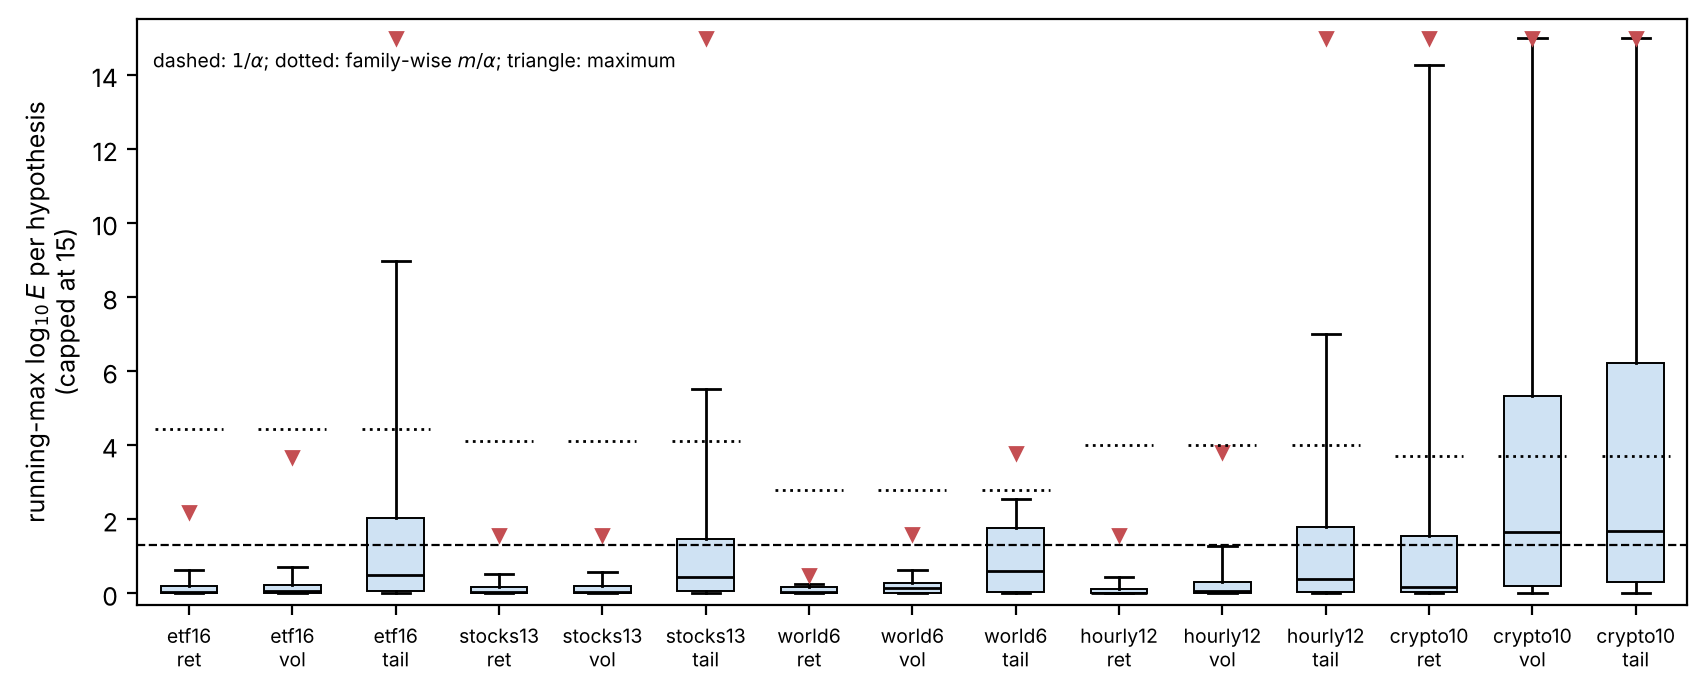
\includegraphics[width=\textwidth]{figures/fig_scan.png}
\caption{\DIFaddFL{Running-maximum evidence $\log_{10}E$ per hypothesis for the lag-$1$ families of each panel and target (box: quartiles, whiskers: $5$th--$95$th percentile, triangle: maximum, dotted line: family-wise threshold, dashed: $1/\alpha$). Returns and volatility stay below the family-wise thresholds in daily panels; stress indicators and crypto do not}}\label{fig:scan}
\end{figure}

\paragraph{\DIFadd{Null calibration on the real data.}} \DIFadd{A simulated null says little about how the test behaves on real series. We therefore calibrate on the data themselves: for a random sample of hypotheses, the target is circularly shifted by at least a year (a quarter, for weekly data) relative to
sources and conditioner, which preserves its marginal law and autocorrelation but destroys every cross-dependence, so every null is true. For daily stock volatility, daily ETF returns, hourly stock volatility and hourly stock returns ($250$, $250$}\DIFaddend , \DIFaddbegin \DIFadd{$250$ }\DIFaddend and \DIFdelbegin \DIFdel{that the financial evidence positively favours the no-synergy hypothesis rather
than merely failing to reject it.}%DIFDELCMD < 

%DIFDELCMD < %%%
\paragraph{\DIFdel{The instrument is powered---including in physics.}} %DIFAUXCMD
\addtocounter{paragraph}{-1}%DIFAUXCMD
\DIFdel{The first leg is that
ANTE detects group synergy wherever it genuinely exists, on data outside our own
simulations. The turbulent energy cascade is a canonical physical example of
genuine multi-scale synergy: energy injected at large scales flows to }\DIFdelend \DIFaddbegin \DIFadd{$200$ hypotheses), the distribution of the running maximum
under the placebo coincides with the real one up to the extreme tail (Fig.~\ref{fig:placebo}); raw rejections are $2/250$ (real) versus $0/250$ (placebo) for stock volatility, $2/250$ versus $0/250$ for ETF returns, $10/250$ versus $9/250$ for hourly volatility
(placebo rate $0.036$ $[0.019,0.067]$) and $1/200$ versus $1/200$ for hourly returns. Across nine further returns-and-volatility families (lag $5$, weekly, contemporaneous and lag-$1$ variants, $150$ hypotheses each) the placebo rejects in at most $2/150$ hypotheses ($0.013$) against at most $4/150$ for the real series. The real evidence in these settings therefore sits on the placebo null, which is a more convincing calibration than comparison with a simulated null. It also explains why the median final $\log_{10}E$ is negative: with the present test the simulated null median is $-0.15$,
the placebo median $-0.20$ to $-0.26$ and the real financial median $-0.27$ ($150$ real triples). The drift concentrates in the first third of }\DIFaddend the \DIFdelbegin \DIFdel{smallest
dissipative scales through the joint action of intermediate scales. On the SURD
turbulence dataset (four scale-resolved energy signals, $\sim$21}%DIFDELCMD < {%%%
\DIFdel{, }%DIFDELCMD < }%%%
\DIFdel{760 samples), we
run the $k$-way test of Proposition~\ref{prop:kway} with the three coarser scales
as the group and the finest scale as the target.
ANTE detects the 3-way group
synergy decisively, crossing $1/\alpha$ at $t^\star=734$ and reaching
$\log_{10}E=\mathbf{4.0}$ }\DIFdelend \DIFaddbegin \DIFadd{sample (median contribution $-0.17$ for finance, $-0.11$ for the simulated null), where the forgetting learners are still estimating
the larger model, as the out-of-sample penalty of Section~\ref{subsec:cw} predicts, and is not driven by winning bets that later reverse (a running maximum above $0.3$ followed by a final value below $-0.3$ occurs for $13\%$ of finance triples and $8\%$--$11\%$ of simulated nulls).
}

\emph{\DIFadd{Where the calibration fails.}} \DIFadd{The same placebo applied to the families that do reject shows that the test is not calibrated there }\DIFaddend (Fig.~\DIFdelbegin \DIFdel{\ref{fig:multi})---in agreement with SURD's own
decomposition of the same data. On synthetic ground truth, including a
}\emph{\DIFdel{pure}} %DIFAUXCMD
\DIFdel{3-way mechanism $Y=A\cdot B\cdot C$ with no lower-order structure, power is $74$--$100\%$. A null result in finance therefore cannot be attributed to
a blunt instrument: the same test}\DIFdelend \DIFaddbegin \DIFadd{\ref{fig:placebo}). With a true null, hourly crypto returns reject in $76/200$ hypotheses ($0.38$}\DIFaddend , \DIFdelbegin \DIFdel{unchanged, lights up on real physical synergy}\DIFdelend \DIFaddbegin \DIFadd{$[0.32,0.45]$; real data $53/200$) and hourly crypto volatility in $79/200$ ($0.40$; real $108/200$);
binary stress indicators reject in $28/200$ ($0.14$) for the ETF panel, $19/200$ ($0.095$) for the stock panel and $56/200$ ($0.28$) for hourly stocks (real data: $68/200$, $56/200$ and $65/200$). For these targets the prequential null is violated by the learned forecasters (binary or extremely heavy-tailed series, with strong volatility clustering and a nonlinear link between the cross-product features and the target), and
a rejection does not indicate an $A\times B$ interaction. For daily stress indicators the real rejection rates exceed the placebo rates ($0.34$ versus $0.14$; $0.28$ versus $0.095$), which suggests some genuine cross-sectional dependence in tail events beyond the test's own bias, but we cannot separate it from a misspecified forecaster}\DIFaddend .

\begin{figure}[h]
\centering
\DIFdelbeginFL %DIFDELCMD < 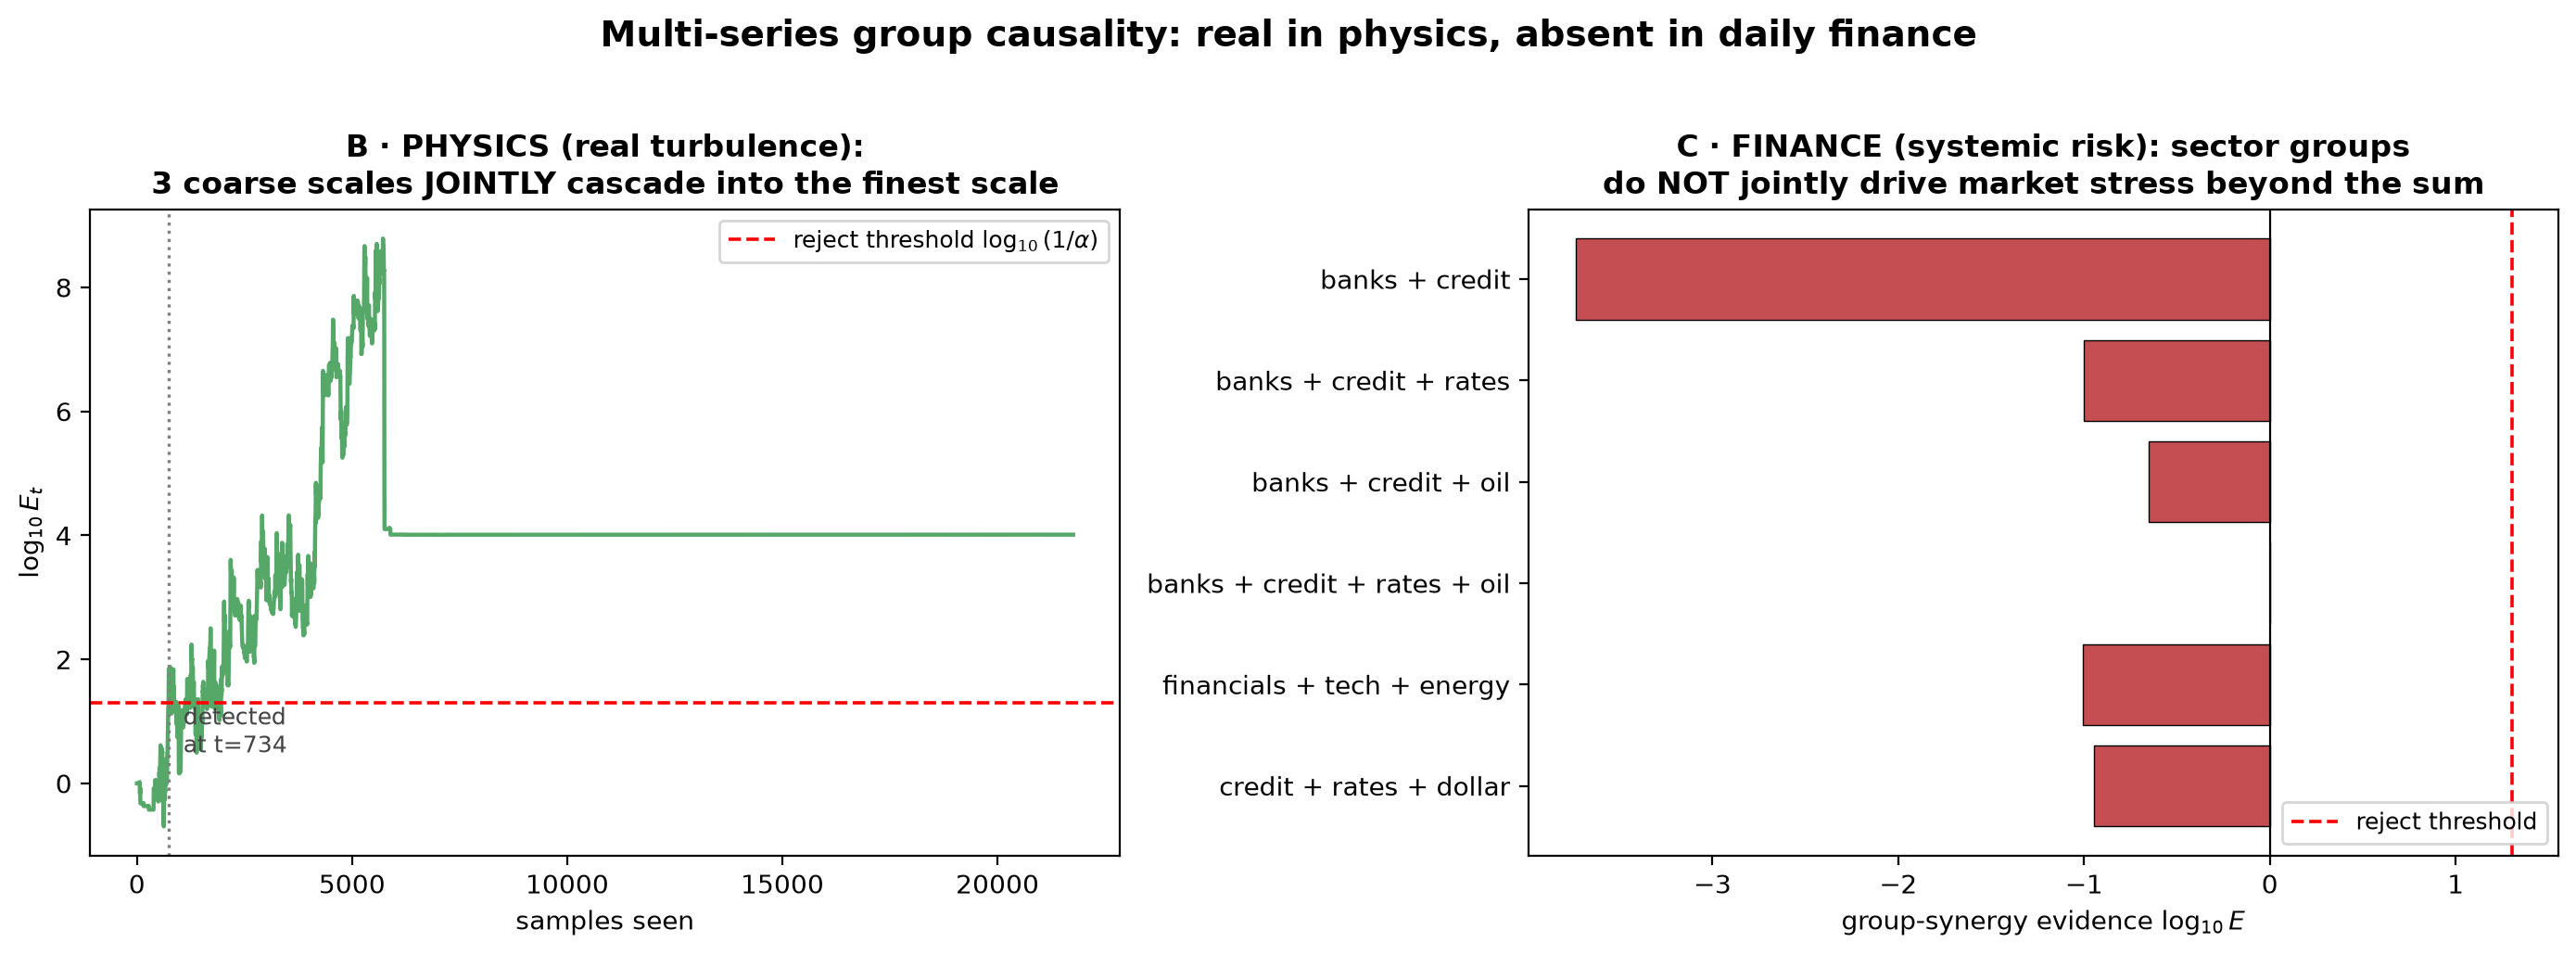
\includegraphics[width=0.9\textwidth]{figures/multiseries_group_causality.png}
%DIFDELCMD < %%%
\DIFdelendFL \DIFaddbeginFL 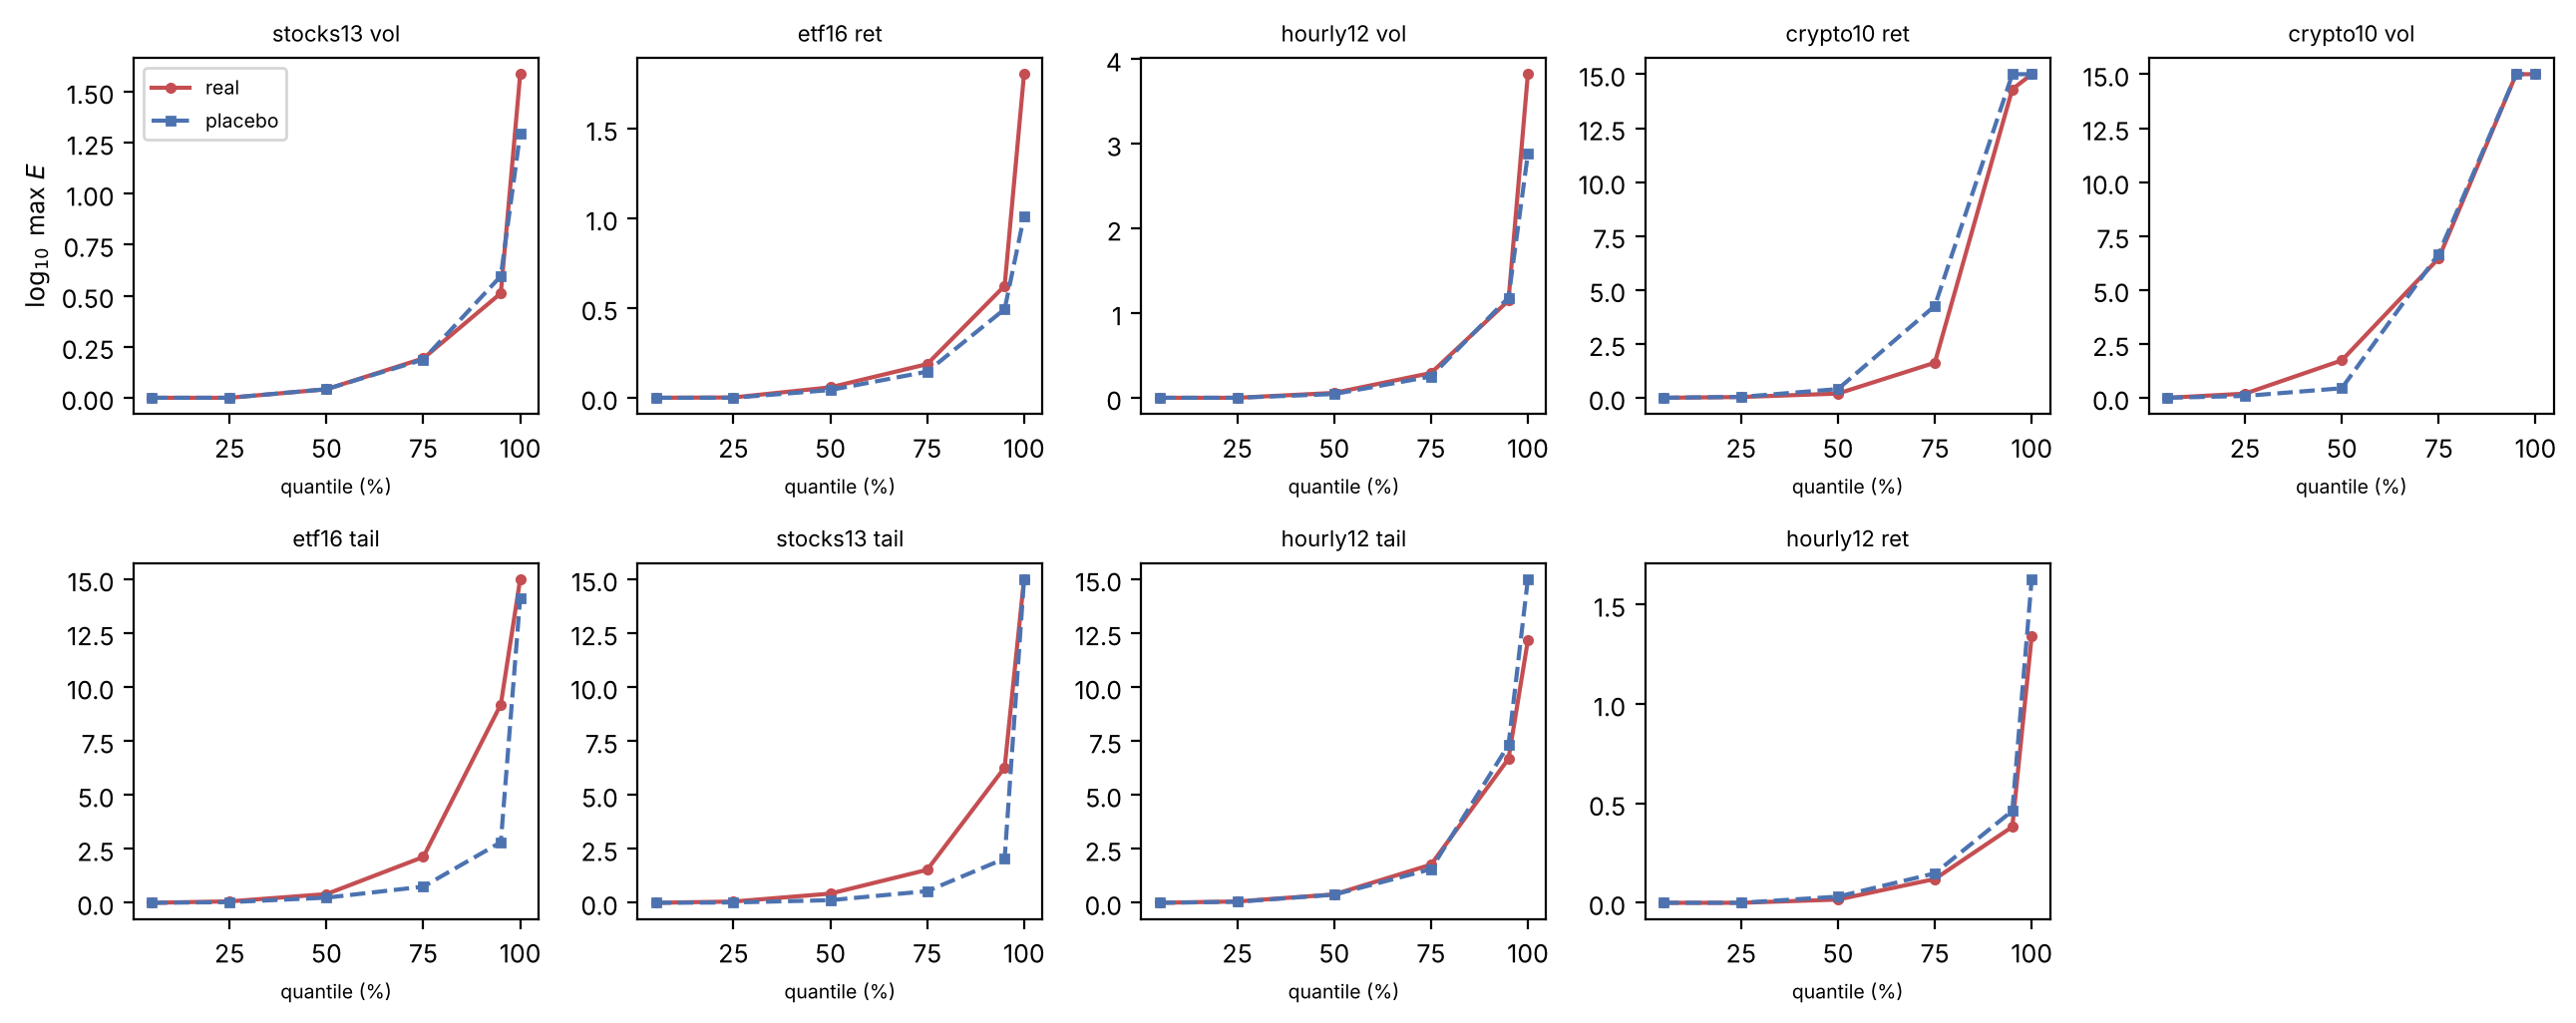
\includegraphics[width=\textwidth]{figures/fig_placebo.png}
\DIFaddendFL \caption{\DIFdelbeginFL \DIFdelFL{The same $k$-way test, two domains. In physics }\DIFdelendFL \DIFaddbeginFL \DIFaddFL{Real versus placebo }\DIFaddendFL (\DIFdelbeginFL \DIFdelFL{turbulence}\DIFdelendFL \DIFaddbeginFL \DIFaddFL{circularly shifted target}\DIFaddendFL ) \DIFaddbeginFL \DIFaddFL{distribution of }\DIFaddendFL the \DIFdelbeginFL \DIFdelFL{capital
process }\DIFdelendFL \DIFaddbeginFL \DIFaddFL{running-maximum evidence }\DIFaddendFL for \DIFaddbeginFL \DIFaddFL{random samples of hypotheses; coinciding curves indicate that real data behave like }\DIFaddendFL the \DIFdelbeginFL \DIFdelFL{3-way energy cascade grows past $1/\alpha$ ($\log_{10}E=4.0$),
establishing genuine group causality. In finance, systemic-risk groups
(banks$+$credit$+$rates, etc.) never accumulate evidence: capital stays flat or
loses money}\DIFdelendFL \DIFaddbeginFL \DIFaddFL{true null in the setting}\DIFaddendFL }\DIFdelbeginFL %DIFDELCMD < \label{fig:multi}
%DIFDELCMD < %%%
\DIFdelendFL \DIFaddbeginFL \label{fig:placebo}
\DIFaddendFL \end{figure}

\paragraph{\DIFdelbegin \DIFdel{Finance matches a true null}\DIFdelend \DIFaddbegin \DIFadd{How much is excluded}\DIFaddend .} The \DIFdelbegin \DIFdel{second leg is that the financial
evidence does not merely fail to reach significance---it }\emph{\DIFdel{positively favours}}
%DIFAUXCMD
\DIFdel{the no-synergy hypothesis. Across $1320$ real financial group triples (a candidate
pair acting on a }\emph{\DIFdel{distinct}} %DIFAUXCMD
\DIFdel{third asset, so that we test genuine group
causality rather than a pair's internal dependence; on volatility and tail-stress
targets; conditioned on the market factor), }\DIFdelend \DIFaddbegin \DIFadd{persistent-alternative e-process of Proposition~\ref{prop:excl} is uninformative on these data, because the learners often agree to within the smallest $\delta$ on the grid ($0.0005$) and the process then wins mechanically. We therefore use the time-uniform bound on }\DIFaddend the \DIFdelbegin \DIFdel{median accumulated evidence is $\log_{10}E=\mathbf{-0.93}$. Because $E_t$ is }\DIFdelend \DIFaddbegin \emph{\DIFadd{running-average}} \DIFadd{conditional synergy of Proposition~\ref{prop:avg}
(loss units; $K=22$ grid points; level $0.05$ divided over the hypotheses of a family; Table~\ref{tab:avgbound} in Appendix~\ref{secA:bounds}). For the lag-$1$ and contemporaneous families of daily returns and volatility, the median hypothesis excludes an average synergy above $0.057$--$0.122$ loss units,
but the least well-bounded hypothesis of a family only excludes values above $0.11$--$2.15$; for lag-$5$ and weekly families, where the forecasters have more regressors or fewer observations, }\DIFaddend the \DIFdelbegin \DIFdel{sceptic's capital, a value below
one means the bet on synergy }\emph{\DIFdel{lost}} %DIFAUXCMD
\DIFdel{money: the }\DIFdelend median \DIFdelbegin \DIFdel{e-value of $\approx0.12$
says a wager on group synergy would, on the typical financial triple, be reduced to
an eighth of its stake.
This is }\DIFdelend \DIFaddbegin \DIFadd{bound is $0.22$--$0.75$ and the worst case is much larger. The realised mean score is negative in every family (median $-0.005$ to $-0.034$ per step), as the out-of-sample penalty predicts.
Because the bound uses the worst-case variance proxy $b_s^2$, it is conservative, and it is weak against magnitudes that are plausible for daily returns (a gain of order $1\%$ of the variance): the data exclude average synergies of }\DIFaddend the \DIFdelbegin \DIFdel{operational meaning of evidence }\emph{\DIFdel{for}} %DIFAUXCMD
\DIFdel{the null. To calibrate it we simulate two references at the identical sample sizes and conditioning---a true-null DGP (additive, common-factor, no interaction)}\DIFdelend \DIFaddbegin \DIFadd{order of several percent of the (truncated) target variance per step, and they do }\emph{\DIFadd{not}} \DIFadd{exclude smaller ones.
}

\paragraph{\DIFadd{Crises.}} \DIFadd{Running e-processes are plotted across whole families in Fig.~\ref{fig:traj}, so that evidence that rises in a crisis and then decays is visible, which a final-value summary would hide. In the $660$ stock-volatility }\DIFaddend and \DIFdelbegin \DIFdel{a
synergy-present DGP---and compare the three distributions
(Table~\ref{tab:eoa}) . The financial distribution sits essentially on top of the true-null (median $\log_{10}E\approx-0.93$ versus $0.00$; detection rate $0.00$
versus the nominal $\approx0.007$}\DIFdelend \DIFaddbegin \DIFadd{$1365$ ETF-return families the maximum over hypotheses of $\log_{10}E_t$ never approaches the family-wise thresholds ($4.1$ and $4.4$): its peak is $1.59$ (January 2017}\DIFaddend ) and \DIFdelbegin \DIFdel{nowhere near the synergy-present
distribution (}\DIFdelend \DIFaddbegin \DIFadd{$2.20$ (5 February 2020, }\emph{\DIFadd{before}} \DIFadd{the COVID sell-off, after which it decays), and during the three windows examined (the 2018 volatility spike, February--June 2020, and 2022) the }\DIFaddend median \DIFdelbegin \DIFdel{$+2.79$, detection rate $0.74$}\DIFdelend \DIFaddbegin \DIFadd{over hypotheses of the within-window maximum is between $-0.10$ and $-0.22$, with only $1.2\%$--$2.2\%$ of hypotheses exceeding $\log_{10}E=0.3$ at any time in a window. The cross-sectional median drifts to about $-0.26$ and the $95$th percentile stays at zero (the bet is switched off}\DIFaddend ).


\DIFdelbegin %DIFDELCMD < \begin{table}[h]
%DIFDELCMD < %%%
\DIFdelendFL \DIFaddbeginFL \begin{figure}[h]
\centering
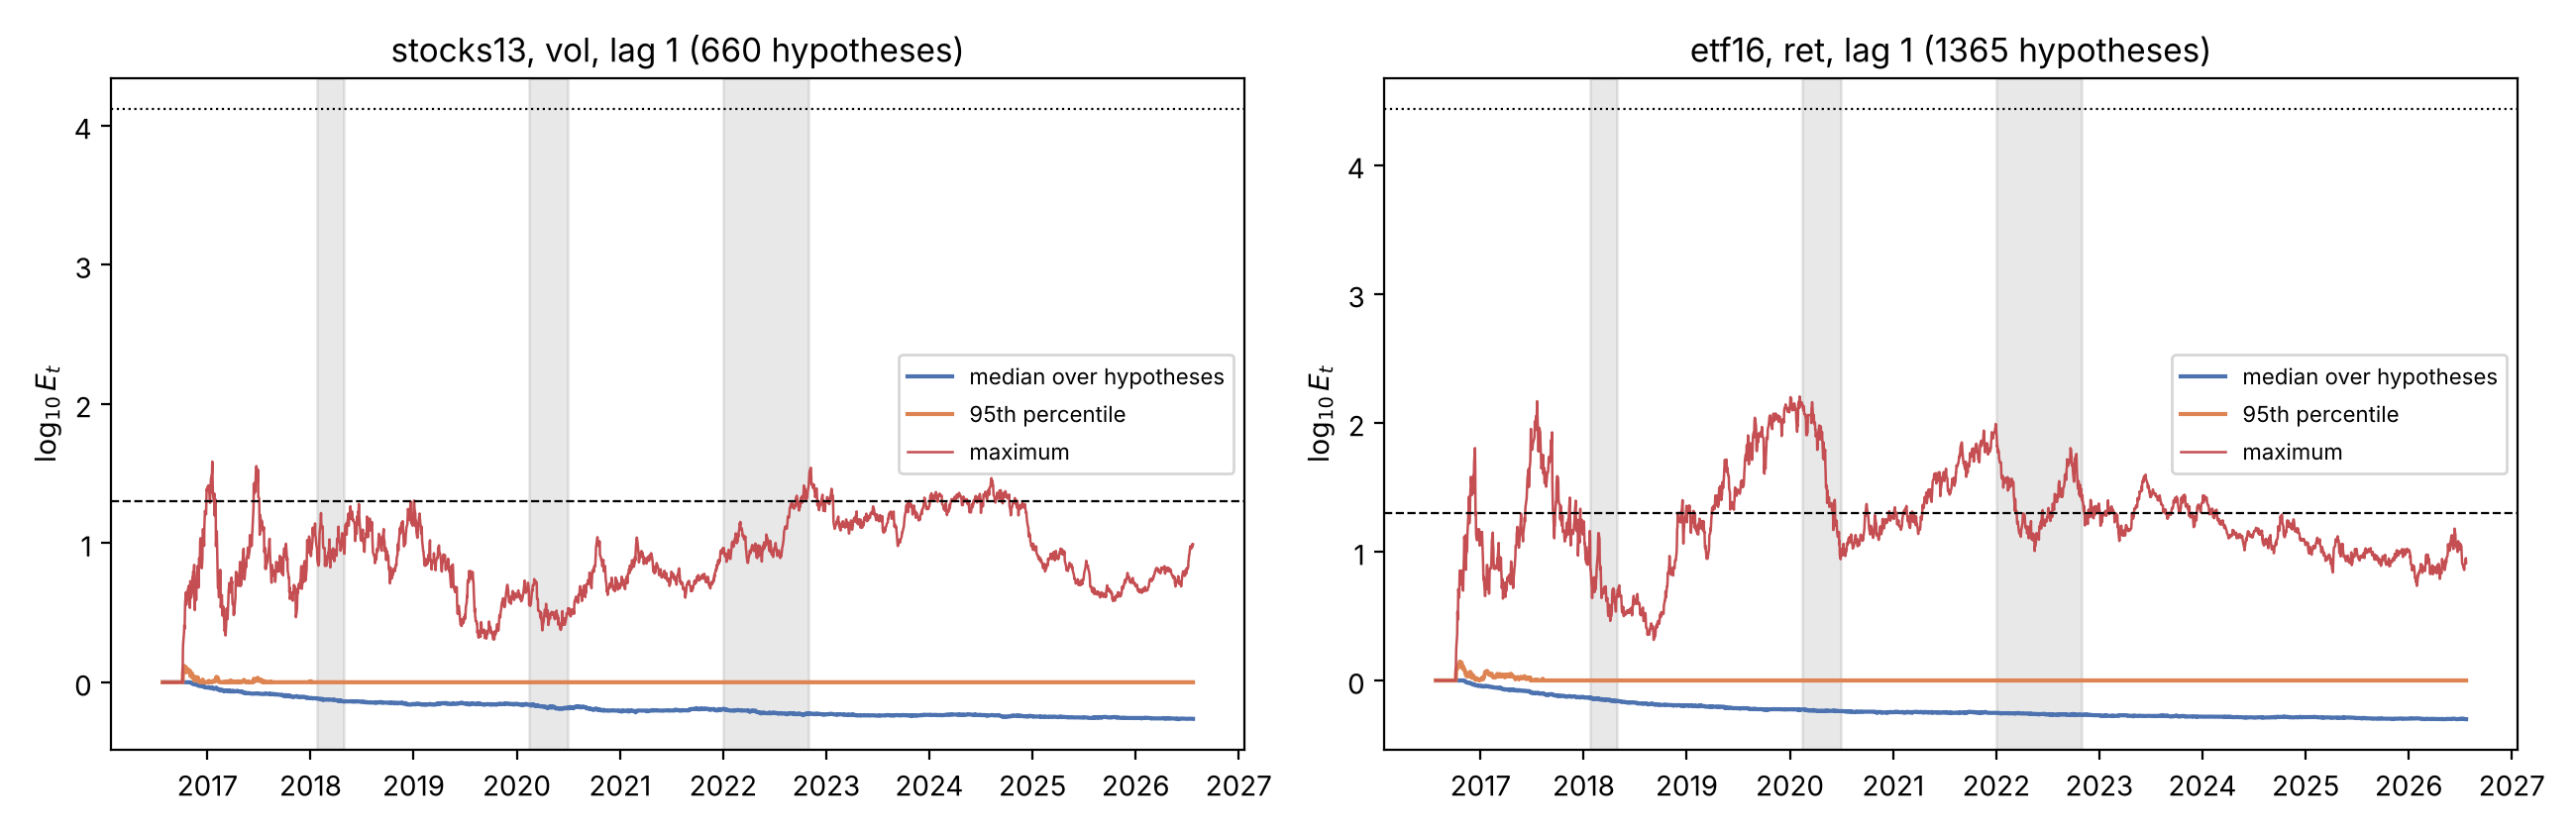
\includegraphics[width=\textwidth]{figures/fig_traj.png}
\DIFaddendFL \caption{\DIFdelbeginFL \DIFdelFL{Evidence of absence. The financial }\DIFdelendFL \DIFaddbeginFL \DIFaddFL{Running }\DIFaddendFL evidence \DIFdelbeginFL \DIFdelFL{distribution sits on top }\DIFdelendFL \DIFaddbeginFL \DIFaddFL{$\log_{10}E_t$ across all hypotheses }\DIFaddendFL of \DIFaddbeginFL \DIFaddFL{two families (median, $95$th percentile, maximum). Shaded: }\DIFaddendFL the \DIFdelbeginFL \DIFdelFL{calibrated true-null and far from }\DIFdelendFL \DIFaddbeginFL \DIFaddFL{2018 volatility spike, }\DIFaddendFL the \DIFdelbeginFL \DIFdelFL{synergy-present distribution. The test
detects synergy with high power where it exists}\DIFdelendFL \DIFaddbeginFL \DIFaddFL{2020 COVID window and 2022; dashed: $1/\alpha$; dotted: family-wise threshold}\DIFaddendFL }\DIFdelbeginFL %DIFDELCMD < \label{tab:eoa}
%DIFDELCMD < \begin{tabular*}{\textwidth}{@{\extracolsep\fill}lccc}
%DIFDELCMD < \toprule
%DIFDELCMD < %%%
\DIFdelFL{Quantity }%DIFDELCMD < & %%%
\DIFdelFL{Real finance }%DIFDELCMD < & %%%
\DIFdelFL{Calibrated true-null }%DIFDELCMD < & %%%
\DIFdelFL{Real synergy }%DIFDELCMD < \\
%DIFDELCMD < \midrule
%DIFDELCMD < %%%
\DIFdelFL{Median evidence $\log_{10}E$ }%DIFDELCMD < & %%%
\DIFdelFL{$\mathbf{-0.93}$ }%DIFDELCMD < & %%%
\DIFdelFL{$0.00$ }%DIFDELCMD < & %%%
\DIFdelFL{$+2.79$ }%DIFDELCMD < \\
%DIFDELCMD < %%%
\DIFdelFL{Detection rate }%DIFDELCMD < & %%%
\DIFdelFL{$\mathbf{0.00}$ }%DIFDELCMD < & %%%
\DIFdelFL{$0.007$ }%DIFDELCMD < & %%%
\DIFdelFL{$0.74$ }%DIFDELCMD < \\
%DIFDELCMD < \botrule
%DIFDELCMD < \end{tabular*}
%DIFDELCMD < \end{table}
%DIFDELCMD < %%%
\DIFdelend \DIFaddbegin \label{fig:traj}
\end{figure}
\DIFaddend 

\paragraph{\DIFdelbegin \DIFdel{The absence is broad }\DIFdelend \DIFaddbegin \DIFadd{Truncation level }\DIFaddend and \DIFdelbegin \DIFdel{robust}\DIFdelend \DIFaddbegin \DIFadd{winsorisation}\DIFaddend .} \DIFdelbegin \DIFdel{A single scan could be an artefact of one target, frequency, or asset universe,
so we searched exhaustively. Group
causality---a group jointly driving a }\emph{\DIFdel{distinct}} %DIFAUXCMD
\DIFdel{target beyond the sum of
parts---was looked for, and found absent, in every regime we could construct:
returns, realised volatility, and tail/stress targets; daily and hourly sampling; US sector ETFs, macro and commodity assets, world equity indices, and intraday
crypto; pairs and $3$- and $4$-way groups; and purpose-built systemic-risk targets
(banks$+$credit$+$rates, financials$+$tech$+$energy, credit$+$rates$+$dollar) . The
totals include a $660$-triple daily volatility scan,
a $660$-triple tail-contagion
scan, a $495$-triple intraday volatility scan and its tail counterpart, and }\DIFdelend \DIFaddbegin \DIFadd{For $200$ random hypotheses from each of daily stock volatility and daily ETF returns, varying the truncation level ($c=2,3,5$) and removing the feature winsorisation changes the raw rejection count by at most two hypotheses ($1$--$2/200$ at $c=2$, $0/200$ for $c=5$ or without winsorisation,
$1/200$ at the default) and the median final $\log_{10}E$ stays between $-0.15$ and $-0.33$; the conclusions for daily returns and volatility are therefore not sensitive to these choices.
}

\paragraph{\DIFadd{Forgetting factor and the Clark--West diagnostic.}} \DIFadd{With forgetting factors from $0.98$ to $0.999$ }\DIFaddend the \DIFdelbegin \DIFdel{$1320$-triple calibrated study above. Across more than $3700$ triples in all, there
were }\emph{\DIFdel{zero}} %DIFAUXCMD
\DIFdel{family-wise detections (Fig.~\ref{fig:eoa}); even the single most
extreme daily-volatility triple fell short of the }\DIFdelend \DIFaddbegin \DIFadd{false-rejection rate is at most $0.010$ in every simulated null cell ($100$ replications each; Wilson upper limits up to $0.054$) and the real-data rejection rate at most $0.047$ ($150$ financial triples, $\rho=0.98$), and the median final
$\log_{10}E$ stays between $-0.04$ and $-0.27$; $\rho=0.98$ makes the learners unstable (the Clark--West adjustment term explodes) and is not recommended. The Clark--West-adjusted mean score is $0.03$--$0.13$ for $\rho\in[0.99,0.999]$ on both simulated and financial data,
which gives the size of the noise floor; as stated in Section~\ref{subsec:cw} we do not use it for inference.
}

\paragraph{\DIFadd{The pairwise layer.}} \DIFadd{\mbox{%DIFAUXCMD
\citet{billio2012} }\hskip0pt%DIFAUXCMD
measure connectedness through pairwise Granger networks. On the same panels, the fraction of significant ordered pairs (Bonferroni at $0.05$) is $0.20$ for ETF returns and $0.78$ for ETF volatility at lag $1$
($0.10$ and $0.61$ for stocks), and a rolling $252$-day window gives a density of up to $0.55$ (ETFs) and $0.40$ (stocks) around the 2020 crash against a median of about $0.1$. Daily markets therefore have a strong pairwise layer, particularly in volatility. For $660$ stock-volatility triples, $145$ have both single-source tests
significant after conditioning on SPY ($29$ after Bonferroni), but only $4$ reach a raw ANTE-SG rejection and none a }\DIFaddend family-wise \DIFdelbegin \DIFdel{threshold. The
interpretation is structural: daily markets are dominated by a common factor and pairwise co-movement, and once those are accounted for , essentially no irreducible
higher-order structure remains that survives an out-of-sample, anytime-valid
criterion.
}\DIFdelend \DIFaddbegin \DIFadd{one: the pairwise structure is not accompanied by detectable super-additive structure.
}\DIFaddend 

\DIFdelbegin %DIFDELCMD < \begin{figure}[h]
%DIFDELCMD < \centering
%DIFDELCMD < 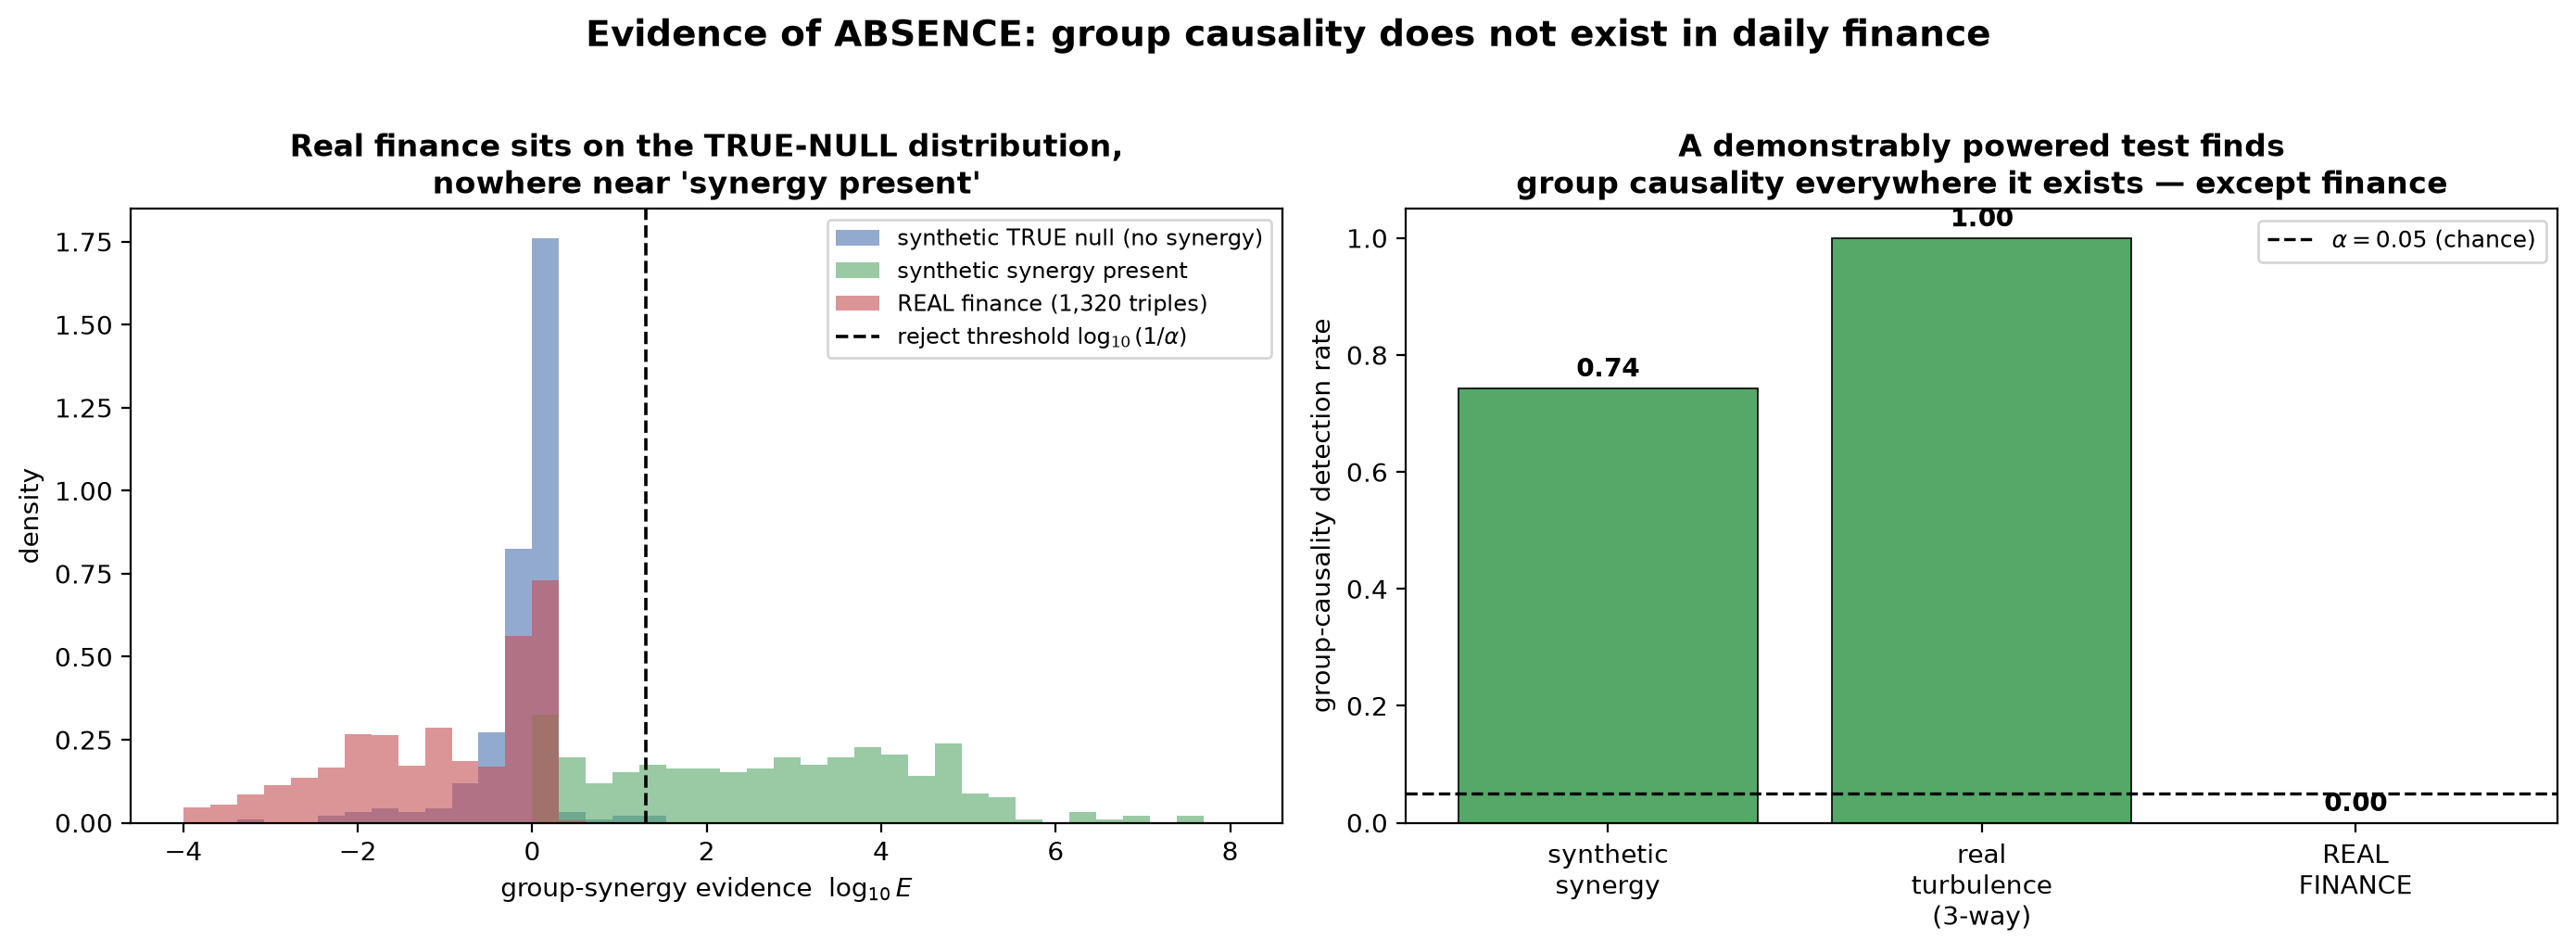
\includegraphics[width=0.9\textwidth]{figures/evidence_of_absence.png}
%DIFDELCMD < %%%
%DIFDELCMD < \caption{%
{%DIFAUXCMD
\DIFdelFL{Evidence of absence. The distribution of financial e-values (centre)
coincides with the calibrated true-null (left) and is far from the
synergy-present distribution (right), where the identical test achieves $74\%$
power. Daily markets carry no irreducible group synergy}}%DIFAUXCMD
%DIFDELCMD < \label{fig:eoa}
%DIFDELCMD < \end{figure}
%DIFDELCMD < %%%
\DIFdelend \DIFaddbegin \subsection{\DIFadd{Interpretation}}\label{subsec:exp-interp}
\DIFaddend 

\DIFdelbegin \DIFdel{This is a substantive statement about market structure and a direct, quantified
caution to the strand of }\DIFdelend \DIFaddbegin \DIFadd{We summarise what the evidence supports, keeping the wording to the searched space. In daily and weekly returns and volatility of the panels examined, for lag $1$, lag $5$ and contemporaneous structures, the ANTE-SG test finds no statistically significant super-additive predictive group effect
at the family-wise level, and }\DIFaddend the \DIFdelbegin \DIFdel{synergy-in-finance literature that reports such
effects from in-sample information-theoretic decompositions
\mbox{%DIFAUXCMD
\citep{scagliarini2020}}\hskip0pt%DIFAUXCMD
: under an out-of-sample, anytime-valid test they do not hold. Synergistic group causality is real---turbulence proves it---but it is a
physics/biology phenomenon, not a daily-markets one}\DIFdelend \DIFaddbegin \DIFadd{real-data evidence has the distribution of a placebo null. Where significant evidence does appear (stress indicators; hourly crypto), a placebo test shows that the test rejects a true null in $10$--$40\%$ of hypotheses for these targets, so the rejections are not interpretable as synergy and the test would need a different forecaster or score (binary or heavy-tailed targets) to be usable there;
We do not claim that synergy is absent from financial markets in general, and not even from the settings searched, for three reasons developed above: the test has low power on real financial noise even for large injected interactions (semi-synthetic power), the predictor class limits what can be detected,
and non-rejection is a statement about these online forecasters (Remark~\ref{rem:notpop})}\DIFaddend .

%%==========================================================%%
\section{Discussion and conclusions}\label{sec:discussion}

ANTE reframes synergy detection from estimation to \emph{testing} \DIFdelbegin \DIFdel{, }\DIFdelend and from fixed-sample to \emph{anytime-valid} \DIFaddbegin \DIFadd{inference}\DIFaddend . The methodological \DIFdelbegin \DIFdel{payoff is a guarantee no
prior synergy method offers: continuous monitoring }\DIFdelend \DIFaddbegin \DIFadd{result is a pair of tests }\DIFaddend with time-uniform error control\DIFdelbegin \DIFdel{, on groups, isolating genuine interaction, without stationarity or
correct-specification assumptions}\DIFdelend \DIFaddbegin \DIFadd{: an interventional test under a known randomised design
whose null is sequential and therefore allows nonstationarity, and a predictive test for time series whose null compares two learned forecasters and whose validity proof is exact (Theorem~\ref{thm:sgvalid}) once the score is built from a truncated loss and
a bound that is known before each observation}\DIFaddend . The cost \DIFdelbegin \DIFdel{, made explicit in
Fig.~\ref{fig:bench}, is a modest loss of fixed-$N$ power relative to a calibrated
batch estimator---the standard and honest price of validity under optional
stopping}\DIFdelend \DIFaddbegin \DIFadd{of exactness is a loss of sensitivity to interactions concentrated in rare extreme observations, which we quantified on real noise (Section~\ref{subsec:exp-pv}); a second cost, common to every
anytime-valid procedure, is lower power than an oracle fixed-sample test at a single pre-committed sample size}\DIFaddend .

\DIFdelbegin \DIFdel{The scientific payoff is the evidence-of-absence finding. It is easy to
}\emph{\DIFdel{find}} %DIFAUXCMD
\DIFdel{synergy in-sample: with enough basis functions any joint model
out-fits the sum of marginals on training data. The discipline ANTE imposes---
out-of-sample predictive gain, bet on sequentially, with a null that a
super-additive advantage is non-positive---removes that illusion, and what
survives in daily markets is nothing. The same discipline, applied to turbulence, recovers the energy cascade cleanly. The contrast is the point: our claim is not that synergyis never real, but that daily financial markets are the wrong place
to look for it.
}\DIFdelend \DIFaddbegin \paragraph{\DIFadd{Arguments that do not hold.}} \DIFadd{Three tempting arguments are avoided here. (i) A validity proof for the group score by clipping fails, because clipping does not in general preserve the sign of the conditional mean
(Example~\ref{ex:clipfail}). (ii) Isolation of an interaction from joint dependence does not follow from additivity of the mechanism: it needs orthogonality, which holds under independence or span conditions and can fail when sources are dependent and the mechanism lies outside the feature span (Proposition~\ref{prop:isolation}),
and the four-model contrast is contaminated by redundancy and suppression. (iii) A real-data positive or negative control is only informative if the test has been calibrated against a placebo null on the same kind of data: smooth near-deterministic signals (turbulence), binary stress indicators and hourly crypto series show that the test can reject a true null there.
}\DIFaddend 

\paragraph{Limitations.} \DIFdelbegin \DIFdel{The predictive null tests super-additive
}\emph{\DIFdel{predictability}}%DIFAUXCMD
\DIFdel{, not a structural intervention; the interventional test
requires a known or randomized design (relaxed by the AIPW score of \S\ref{subsec:score}, whose finite-sample behaviour under estimated propensities
we leave to future work).
Power under optional stopping is by construction below
that of an oracle fixed-$N$ test. The financial finding is }\DIFdelend \DIFaddbegin \DIFadd{(1) A rejection means that the joint forecaster had a persistently positive conditional advantage over the additive one (Remark~\ref{rem:notpop}); reading it as an irreducible $A\times B$ interaction needs the conditions of Proposition~\ref{prop:isolation}, which cannot be checked in data, and reading it as causal needs an
interventional design. (2) The prequential null is not implied by zero population synergy, so Type-I control for population-level nulls is established by simulation and placebo calibration, not by theorem; the simulations include heavy tails, GARCH, nonstationarity and correlated sources but are not exhaustive, and the test fails on smooth, near-deterministic signals such as the turbulence data.
(3) Power: the test has low power for lagged interactions between heavy-tailed returns (which relaxing the truncation does not cure), loses power as the two sources become nearly collinear (the interaction is then not identifiable), and its detectable alternatives depend on the dictionary; a random-feature dictionary removes one blind spot but the choice of dictionary is fixed in advance. For the implemented plug-in bet we prove validity only.
(4) Families are not pre-registered and overlap (shared assets, repeated targets), so the e-Bonferroni thresholds, though valid under arbitrary dependence, are conservative. (5) Conclusions are }\DIFaddend specific to the \DIFdelbegin \DIFdel{frequencies and horizons studied (daily and hourly); higher-frequency or
longer-horizon regimes could in principle harbour synergy the present scan would
not see, and we report the searched space rather than claiming universality}\DIFdelend \DIFaddbegin \DIFadd{panels, targets, lag structures and sample periods searched; for hourly crypto data and binary stress indicators the test is not calibrated (Section~\ref{subsec:exp-fin}), so the significant evidence there cannot be interpreted. (6) The augmented (AIPW) interventional score with estimated propensities is an extension without a finite-sample guarantee}\DIFaddend .

\paragraph{Future work.} \DIFdelbegin \DIFdel{Nonlinear (kernel or neural ) predictors }\DIFdelend \DIFaddbegin \DIFadd{Kernel or neural forecasters }\DIFaddend in the same betting scaffold\DIFdelbegin \DIFdel{; the doubly-robust and graph/GNN instantiations sketched in
\S\ref{subsec:score}; and the }\DIFdelend \DIFaddbegin \DIFadd{, together with the sequential kernelised tests of \mbox{%DIFAUXCMD
\citet{podkopaev2023}}\hskip0pt%DIFAUXCMD
; anytime-valid conditional-independence tests \mbox{%DIFAUXCMD
\citep{grunwald2024ci} }\hskip0pt%DIFAUXCMD
to condition on confounders and move from predictive to causal readings;
a sequential comparison with regret guarantees for the plug-in bet; and an }\DIFaddend information-theoretic instantiation \DIFdelbegin \DIFdel{, }\DIFdelend in which a permutation-recentred PEID increment is bet on\DIFdelbegin \DIFdel{to give the first }\emph{\DIFdel{sequential}}
%DIFAUXCMD
\DIFdel{synergy monitor on the information scale}\DIFdelend .

\paragraph{Conclusion.} We introduced ANTE, \DIFdelbegin \DIFdel{the first }\DIFdelend \DIFaddbegin \DIFadd{an }\DIFaddend anytime-valid \DIFdelbegin \DIFdel{, nonparametric, }\DIFdelend sequential test of \DIFdelbegin \DIFdel{synergistic (group ) causality. Built on testing-by-betting, it }\DIFdelend \DIFaddbegin \DIFadd{group synergy with an interventional and a predictive formulation. It }\DIFaddend controls Type-I error uniformly over all stopping times \DIFdelbegin \DIFdel{(Theorem~\ref{thm:validity} ,
Corollary~\ref{cor:anytime}), rejects with probability one under any persistent
super-additive alternative with an explicit $\delta^{-2}$ }\DIFdelend \DIFaddbegin \DIFadd{for the sequential null of the interventional part and for the forecaster-comparison null of the predictive part (Theorems~\ref{thm:validity} and~\ref{thm:sgvalid}); for population-level nulls in real data, control is established only by simulation and placebo calibration. The test has power one and a high-probability }\DIFaddend detection-time bound \DIFaddbegin \DIFadd{for an oracle bet }\DIFaddend (Theorem~\ref{thm:consistency}, Proposition~\ref{prop:latency}), extends to $k$-way groups (\DIFdelbegin \DIFdel{Proposition~\ref{prop:kway}}\DIFdelend \DIFaddbegin \DIFadd{Corollary~\ref{cor:group}}\DIFaddend ), and \DIFdelbegin \DIFdel{provably isolates genuine
interaction from joint dependence and own-nonlinearity
}\DIFdelend \DIFaddbegin \DIFadd{comes with an exclusion e-process, a time-uniform bound on average synergy and a precise account of what a rejection means }\DIFaddend (Proposition~\ref{prop:isolation}).
Empirically it \DIFdelbegin \DIFdel{matches state-of-the-art batch
estimators in detection while being the only method that monitors continuously
with valid error control. Turned on real data as a powered instrument, ANTE
establishes that }\DIFdelend \DIFaddbegin \DIFadd{holds its level under continuous monitoring and under a range of stress nulls, and in a fully specified search of financial data it finds no statistically significant }\DIFaddend super-additive \DIFdelbegin \DIFdel{group causality is absent from daily financial
markets, while it detects the turbulent energy cascade in physics. The tool and the finding are, we hope, of independent value:
the tool, wherever streaming
group-causality decisions must be made under continuous monitoring; the finding,
as a quantified correction to synergy-in-finance claims}\DIFdelend \DIFaddbegin \DIFadd{predictive group effect in daily and weekly returns and volatility, with real-data evidence that matches a placebo null. The methodological result and the empirical finding are separate:
the first is a theorem and simulation record; the second is a finding about the specific panels searched}\DIFaddend .

\backmatter

\bmhead{Supplementary information}
Code, data \DIFdelbegin \DIFdel{, and scripts reproducing }\DIFdelend \DIFaddbegin \DIFadd{and scripts that reproduce }\DIFaddend every figure and table are available in the
public repository (\DIFdelbegin \DIFdel{\S\ref{sec:decl}}\DIFdelend \DIFaddbegin \DIFadd{see Declarations}\DIFaddend ).

\bmhead{Acknowledgements}
The \DIFdelbegin \DIFdel{authors }\DIFdelend \DIFaddbegin \DIFadd{author }\DIFaddend received no specific funding for this work.

\section*{\DIFdelbegin \DIFdel{Statements and }\DIFdelend Declarations}\label{sec:decl}

\DIFdelbegin \paragraph{\DIFdel{Funding.}} %DIFAUXCMD
\addtocounter{paragraph}{-1}%DIFAUXCMD
\DIFdelend \DIFaddbegin \subsection*{\DIFadd{Ethical approval}}
\DIFadd{Not applicable. This study uses only publicly available market and turbulence (fluid-dynamics)
data and synthetic simulations. It involves no human participants, human data or animals,
and no ethical approval was required.
}

\subsection*{\DIFadd{Consent to participate}}
\DIFadd{Not applicable. The study involved no human participants.
}

\subsection*{\DIFadd{Consent to publish}}
\DIFadd{Not applicable. The manuscript contains no individual person's data, images or details
that would require consent for publication.
}

\subsection*{\DIFadd{Funding}}
\DIFaddend No funding was received to assist with the preparation of this manuscript.

\DIFdelbegin \paragraph{\DIFdel{Competing interests.}} %DIFAUXCMD
\addtocounter{paragraph}{-1}%DIFAUXCMD
\DIFdel{The authors have }\DIFdelend \DIFaddbegin \subsection*{\DIFadd{Competing interests}}
\DIFadd{The author has }\DIFaddend no competing interests to declare that are relevant to the content of this
article.

\DIFdelbegin \paragraph{\DIFdel{Ethics approval.}} %DIFAUXCMD
\addtocounter{paragraph}{-1}%DIFAUXCMD
\DIFdel{Not applicable. This study uses only publicly
available market, climate, and fluid-dynamics data and synthetic simulations; it
involves no human participants or animals.
}%DIFDELCMD < 

%DIFDELCMD < %%%
\paragraph{\DIFdel{Data availability.}} %DIFAUXCMD
\addtocounter{paragraph}{-1}%DIFAUXCMD
\DIFdelend \DIFaddbegin \subsection*{\DIFadd{Data availability}}
\DIFaddend All datasets are public\DIFdelbegin \DIFdel{: financial }\DIFdelend \DIFaddbegin \DIFadd{. Financial }\DIFaddend series were obtained from the Yahoo Finance chart API \DIFdelbegin \DIFdel{, climate teleconnection indices from
NOAA PSL, }\DIFdelend and the turbulence energy-cascade signals \DIFaddbegin \DIFadd{(used only in a placebo check) }\DIFaddend from
the released SURD repository \citep{surd2024}. Downloaders and processed \DIFdelbegin \DIFdel{CSVs }\DIFdelend \DIFaddbegin \DIFadd{CSV files }\DIFaddend are included in the
project repository\DIFdelbegin \DIFdel{at }%DIFDELCMD < \url{https://github.com/vinhqdang/REIGN_Regime-Enhanced-Intelligent-Granger-Network}
%DIFDELCMD < %%%
\DIFdel{(the ANTE code and data reside in the }\texttt{\DIFdel{sequential-synergy-causality/}}
%DIFAUXCMD
\DIFdel{subdirectory )}\DIFdelend \DIFaddbegin \DIFadd{,
}\href{https://github.com/vinhqdang/REIGN_Regime-Enhanced-Intelligent-Granger-Network}{\texttt{\DIFadd{github.com/vinhqdang/REIGN\_Regime-Enhanced-Intelligent-Granger-Network}}}\DIFadd{,
in the subdirectory }\texttt{\DIFadd{sequential-synergy-causality/}}\DIFaddend .

\DIFdelbegin \paragraph{\DIFdel{Code availability.}} %DIFAUXCMD
\addtocounter{paragraph}{-1}%DIFAUXCMD
\DIFdelend \DIFaddbegin \subsection*{\DIFadd{Code availability}}
\DIFaddend All source code (the ANTE and ANTE-SG implementations \DIFaddbegin \DIFadd{including the revised test
}\texttt{\DIFadd{src/ante\_v2.py}}\DIFaddend , the re-implemented baselines, the experiment scripts \DIFaddbegin \DIFadd{under
}\texttt{\DIFadd{experiments/revision/}}\DIFaddend , and the figure-generation code) is openly released \DIFdelbegin \DIFdel{in the same repository,
}%DIFDELCMD < \url{https://github.com/vinhqdang/REIGN_Regime-Enhanced-Intelligent-Granger-Network}%%%
\DIFdelend \DIFaddbegin \DIFadd{at
}\href{https://github.com/vinhqdang/REIGN_Regime-Enhanced-Intelligent-Granger-Network}{\texttt{\DIFadd{github.com/vinhqdang/REIGN\_Regime-Enhanced-Intelligent-Granger-Network}}}\DIFaddend , under
\texttt{sequential-synergy-causality/}. \DIFaddbegin \DIFadd{The experiments were run with Python 3.13.16 using
NumPy 2.5.3, SciPy 1.18.1, pandas 3.0.5 and Matplotlib 3.11.2 on a four-core Linux container; all random number
generators are seeded, and the seeds are given in the scripts.
}\DIFaddend 

\DIFdelbegin \paragraph{\DIFdel{Author contributions.}} %DIFAUXCMD
\addtocounter{paragraph}{-1}%DIFAUXCMD
\DIFdelend \DIFaddbegin \subsection*{\DIFadd{Author contributions}}
\DIFaddend Q.-V.~Dang is the sole author and conceived the method, developed the theory, implemented the
algorithms and experiments, and wrote the manuscript.

\begin{appendices}

\section{Proofs \DIFaddbegin \DIFadd{and supporting results}\DIFaddend }\label{secA:proofs}

\DIFdelbegin \subsection*{\DIFdel{Proof of Theorem~\ref{thm:consistency}}}
%DIFAUXCMD
\DIFdelend \DIFaddbegin \DIFadd{Throughout, ``predictable'' means $\F_{t-1}$-measurable, $\gamma<1$, and Ville's inequality is
used in the form: if $(M_t)_{t\ge0}$ is a nonnegative supermartingale with $\E M_0\le1$ then
$\Prob(\exists t:M_t\ge1/\alpha)\le\alpha$.
}

\subsection*{\DIFadd{A.1 Proofs for Part A}}

\begin{proof}[Proof of Lemma~\ref{lem:unbiased}]
\DIFadd{Write $\psi_t=\sum_{a,b}c(a,b)\indic\{A_t=a,B_t=b\}C_t(a,b)/\pi_t(a,b)$. Condition on
$(\mathcal H_t,\{C_t(\cdot)\})$. By sequential randomisation each term has conditional mean
$c(a,b)C_t(a,b)$, because $\pi_t$ is $\mathcal H_t$-measurable. Taking $\E[\cdot\mid\mathcal H_t]$ gives
$\theta_t(X_t)$, and the tower property gives $\E[\psi_t\mid\F_{t-1}]=\theta_t$. The bound follows from
$0\le C_t\le1$ and positivity.
}\end{proof}

\begin{proof}[Proof of Theorem~\ref{thm:validity} and Corollary~\ref{cor:anytime}]
\DIFadd{Each factor $1+\lambda_t\psi_t\ge1-\gamma>0$, so $E_t\in(0,(1+\gamma)^t]$ is integrable. Since $\lambda_t$ is predictable,
$\E[E_t\mid\F_{t-1}]=E_{t-1}(1+\lambda_t\theta_t)$. Under $H_0^{\le}$ and $\lambda_t\ge0$ this is at
most $E_{t-1}$. Under $H_0^{=}$ it equals $E_{t-1}$, and an average of two martingales for the
same filtration is a martingale. Ville's inequality gives the crossing bound, and optional stopping
for nonnegative supermartingales gives $\E E_\tau\le1$ for every stopping time.
}\end{proof}

\begin{proof}[Proof of Lemma~\ref{lem:log}]
\DIFadd{Put $q(x)=(x-\log(1+x))/x^2=\int_0^1v/(1+xv)\,dv$ for $x>-1$; $q$ is strictly decreasing, so
$q(x)\le q(-\gamma)=C_\gamma$ on $[-\gamma,\infty)$, with equality at $-\gamma$. Finally
$q(-\gamma)=\int_0^1v/(1-\gamma v)dv\le1/(2(1-\gamma))$.
}\end{proof}

\begin{proof}[Proof of Theorem~\ref{thm:consistency}]
\DIFaddend Let $W_s=\log(1+\lambda\psi_s)$. Since \DIFdelbegin \DIFdel{$|\lambda\psi_s|\le\gamma<1$, $W_s$ is
bounded: $|W_s|\le\log\frac{1}{1-\gamma}$.
Using $\log(1+x)\ge x-\tfrac{x^2}
{2(1-\gamma)}$ for $x\ge-\gamma$, }%DIFDELCMD < \[
%DIFDELCMD < \E[W_s\mid\F_{s-1}]\ \ge\ \lambda\,\E[\psi_s\mid\F_{s-1}]-\frac{\lambda^2}{2(1-\gamma)}\E[\psi_s^2\mid\F_{s-1}]\ \ge\ \lambda\delta-\frac{\lambda^2c_\psi^2}{2(1-\gamma)},
%DIFDELCMD < \]
%DIFDELCMD < %%%
\DIFdel{using Assumption~\ref{ass:alt} and $\psi_s^2\le c_\psi^2$. Absorbing the harmless
$(1-\gamma)^{-1}$ into the
constant (or restricting to small $\lambda$ where
$\log(1+x)\ge x-x^2$ on $[-\tfrac12,\tfrac12]$) gives the stated lower bound$\lambda\delta-\tfrac12\lambda^2c_\psi^2=:g_0>0$ for $\lambda<2\delta/c_\psi^2$}\DIFdelend \DIFaddbegin \DIFadd{$|\lambda\psi_s|\le\bar\gamma$, Lemma~\ref{lem:log} gives
$\E[W_s\mid\F_{s-1}]\ge\lambda\delta-C_{\bar\gamma}\lambda^2c^2=g_0$}\DIFaddend . The differences
$D_s=W_s-\E[W_s\mid\F_{s-1}]$ are \DIFdelbegin \DIFdel{bounded martingale differences ,
so by the strong law for martingales }\DIFdelend \DIFaddbegin \DIFadd{martingale differences bounded by
$\ell_\lambda=\log\frac{1+\lambda c}{1-\lambda c}$, so $\sum_s\E D_s^2/s^2<\infty$ and the martingale
strong law gives }\DIFaddend $t^{-1}\sum_{s\le t}D_s\to0$ a.s. \DIFdelbegin \DIFdel{; hence
$t^{-1}\log E_t=t^{-1}\sum_{s\le t}W_s\to g(\lambda)\ge g_0>0$ }\DIFdelend \DIFaddbegin \DIFadd{Hence
$\liminf t^{-1}\log E_t\ge g_0$ }\DIFaddend a.s. \DIFdelbegin \DIFdel{Therefore $\log E_t\to+\infty$}\DIFdelend \DIFaddbegin \DIFadd{The statement for the cap-based Kelly bet follows by
substituting $\lambda^\star=\delta(1-\gamma)/c^2$ and the bound $C_{\bar\gamma}\le1/(2(1-\gamma))$.
(Almost-sure }\emph{\DIFadd{convergence}} \DIFadd{of $t^{-1}\log E_t$ would need an ergodicity assumption; the
$\liminf$ statement does not.)
}\end{proof}

\begin{proof}[Proof of Proposition~\ref{prop:latency}]
\DIFadd{$\{\tau_\alpha>t\}\subseteq\{\log E_t<\log(1/\alpha)\}$ and $\log E_t\ge tg_0+M_t$ with
$M_t=\sum_{s\le t}D_s$. Each $D_s$ lies in a predictable interval of length $\ell_\lambda$}\DIFaddend , so
\DIFdelbegin \DIFdel{$E_t\ge1/\alpha$ for all large $t$ and the test rejects with probability one.
}%DIFDELCMD < \qed
%DIFDELCMD < %%%
\DIFdelend \DIFaddbegin \DIFadd{Azuma--Hoeffding \mbox{%DIFAUXCMD
\citep{azuma1967} }\hskip0pt%DIFAUXCMD
gives $\Prob(M_t\le-\epsilon)\le\exp(-2\epsilon^2/(t\ell_\lambda^2))$;
take $\epsilon=tg_0-\log(1/\alpha)>0$. For $t\ge2\log(1/\alpha)/g_0$ the exponent is at least
$tg_0^2/(2\ell_\lambda^2)$, which exceeds $\log(1/\beta)$ once $t\ge2\ell_\lambda^2\log(1/\beta)/g_0^2$.
(Using the range at the cap, $\log\frac{1+\gamma}{1-\gamma}$, in place of $\ell_\lambda$ is valid but
gives a bound of order $\delta^{-4}$.)
}\end{proof}
\DIFaddend 

\DIFdelbegin \subsection*{\DIFdel{Proof of Proposition~\ref{prop:latency}}}
%DIFAUXCMD
\DIFdel{By Theorem~\ref{thm:consistency}, $t^{-1}\log E_t\to g>0$ a }\DIFdelend \DIFaddbegin \begin{proof}[Proof of Proposition~\ref{prop:mixture}]
\DIFadd{An average of supermartingales for one filtration is a supermartingale; a sum of nonnegative
terms is at least its largest term, so $E^{\mathrm{mix}}_t\ge K^{-1}\max_jE_t(\lambda_j)$. On the geometric grid,
$g_0$ is a concave quadratic with maximiser $\lambda^\star$, so some grid point in
$[\lambda^\star/2,\lambda^\star]$ has $g_0\ge\tfrac34g_0(\lambda^\star)$}\DIFaddend .
\DIFdelbegin \DIFdel{s.
Fix
$\eta\in(0,g)$; a }\DIFdelend \DIFaddbegin \end{proof}

\paragraph{\DIFadd{Known-design AIPW.}} \DIFadd{Conditioning as in Lemma~\ref{lem:unbiased}, the weighted residual term
of $\phi_t$ has conditional mean $\sum c(a,b)(\E[C_t(a,b)\mid\mathcal H_t]-\hat\mu_{ab,t})$ and the
$\hat\mu$ terms cancel, so $\E[\phi_t\mid\mathcal H_t]=\theta_t(X_t)$ for any $\F_{t-1}$-measurable $\hat\mu$.
One indicator is nonzero, contributing at most $1/\pi_{\min}$, and $|\sum c\,\hat\mu|\le2$, so
$|\phi_t|\le1/\pi_{\min}+2$}\DIFaddend .
\DIFdelbegin \DIFdel{s. \ there is a finite $T_\eta$ with $\log E_t\ge(g-\eta)t$ for $t\ge T_\eta$.
The rejection time satisfies $E_{\tau_\alpha}\ge1/\alpha$, i}\DIFdelend \DIFaddbegin 

\subsection*{\DIFadd{A.2 Proofs for Part B}}

\paragraph{\DIFadd{Why the clipped score fails (Example~\ref{ex:clipfail}).}} \DIFadd{Let $s_t$ be i.i.d.\ with the law in the
example and bet a fixed $\lambda=0.1$ on $u_t=\clip(s_t,-5,5)$. Then
$t^{-1}\log E_t\to0.1\log(1-5\lambda)+0.9\log(1+1.5\lambda)=0.0565>0$ a.s., so $E_t\to\infty$ although
$\E s_t=-0.65$. The plug-in bet behaves identically: $\hat\mu/\hat v\to0.188$ exceeds the cap $0.1$, so $\lambda_t=0.1$
eventually. A data-dependent scale does not repair this: $\Prob(s=-100)=0.01$, $\Prob(s=1)=0.99$ has $\E s=-0.01$, root
mean square $10.05$ and, with $b=5$, $\E\,\clip(s/\mathrm{RMS},-5,5)=+0.0485$; and
$\Prob(s=-1000)=0.001$, $\Prob(s=0.99)=0.999$ with $b=10$ has $\E s=-0.011$, RMS $31.6$ and clipped mean $+0.0213$.
Two sufficient conditions do exist. Writing $m_t=\E[s_t\mid\F_{t-1}]$, $\sigma$ for the scale and
$U_t=\E[(s_t-b\sigma)_+\mid\F_{t-1}]$, $L_t=\E[(-s_t-b\sigma)_+\mid\F_{t-1}]$, one has the exact identity
$\sigma\,\E[\clip(s_t/\sigma,-b,b)\mid\F_{t-1}]=m_t-U_t+L_t$, so the raw null implies the clipped null if and
only if $L_t\le U_t-m_t$. In particular, if the conditional law of $s_t$ is symmetric about $m_t$, then $m_t\le0$ implies
the clipped mean is $\le0$ for every predictable $\sigma>0$ and $b>0$ (the map $x\mapsto\int\clip(x+z)Q(dz)$ is nondecreasing and
vanishes at $0$ for symmetric $Q$). The null stated on the clipped score itself is always valid
(supermartingale by the argument below), but it is not the scientific null.
}

\begin{lemma}[Predictable bound]\label{lem:bound}
\DIFadd{For $\ell_c(e)=\min(e^2,c^2)$ and any $y,p^1,p^2$,
$|\ell_c(y-p^1)-\ell_c(y-p^2)|\le c^2-(c-|p^1-p^2|)_+^2\le\min\{2c|p^1-p^2|,c^2\}$, and the first bound is attained.
}\end{lemma}
\begin{proof}
\DIFadd{$\ell_c(e)=h(|e|)$ with $h(r)=\min(r^2,c^2)$, which is $2c$-Lipschitz, and $||e|-|e'||\le|e-e'|$; this gives the
$2c|p^1-p^2|$ bound. For the sharp bound take $r_1=|y-p^1|\le r_2=|y-p^2|\le r_1+d$ with $d=|p^1-p^2|$; the difference
$\min(r_2,c)^2-\min(r_1,c)^2$ is at most $\min(r_1+d,c)^2-\min(r_1,c)^2$, which is maximised over $r_1$
at $c^2-(c-d)_+^2$}\DIFaddend .
\DIFdelbegin \DIFdel{e.$\log E_{\tau_\alpha}\ge\log(1/\alpha)$; combining with the linear lower bound
gives $\tau_\alpha\le\log(1/\alpha)/(g-\eta)$ once past $T_\eta$. Optimising the lower bound $g_0(\lambda)=\lambda\delta-\tfrac12\lambda^2c_\psi^2$ over $\lambda$
yields $\lambda^\star=\delta/c_\psi^2$ and$g_0(\lambda^\star)=\delta^2/(2c_\psi^2)$, so $\tau_\alpha\lesssim 2c_\psi^2\log(1/\alpha)/\delta^2$.
}%DIFDELCMD < \qed
%DIFDELCMD < %%%
\DIFdelend \DIFaddbegin \end{proof}
\DIFaddend 

\DIFdelbegin \subsection*{\DIFdel{Proof of Proposition~\ref{prop:isolation}}}
%DIFAUXCMD
\DIFdel{Consider the population least-squares predictors over the
feature classes
described. Write the target as $Y_t=f(\mathcal A_t)+h(\mathcal B_t)+\varepsilon_t$
with $\varepsilon_t$ mean-zero given the past and $\mathcal A_t,\mathcal B_t$ the
respective source histories. The $A$-model's feature span contains the projection
of $f(\mathcal A_t)$ realisable from $A$'s linear and quadratic lags; denote its
residual $r^A_t$, orthogonal to the $A$-features. Symmetrically for $B$.
The joint
model additionally spans cross-products $A_{t-\ell}B_{t-\ell}$. Under the additive
DGP the optimal joint coefficients on the cross-products are zero, because the }\DIFdelend \DIFaddbegin \begin{proof}[Proof of Theorem~\ref{thm:sgvalid} and Corollary~\ref{cor:group}]
\DIFadd{By Lemma~\ref{lem:bound}, $|s_t|\le b_t$ for every outcome, so $|u_t|\le1$ and $s_t$ is integrable. Because $b_t$ and
$\indic\{b_t>\varepsilon\}$ are predictable (functions of predictions made before $Y_t$ is seen),
$\E[u_t\mid\F_{t-1}]=\indic\{b_t>\varepsilon\}\E[s_t\mid\F_{t-1}]/b_t\le0$ under $H_0^{\mathrm{preq}}$.
With $\lambda_t\in[0,\gamma]$ predictable, $1+\lambda_tu_t\ge1-\gamma>0$ and
$\E[E_t\mid\F_{t-1}]=E_{t-1}(1+\lambda_t\E[u_t\mid\F_{t-1}])\le E_{t-1}$. Ville's inequality applies. For the capped
process, $x\mapsto\min(x,C)$ is concave, so by Jensen $\E[E'_t\mid\F_{t-1}]\le\min\{E'_{t-1}(1+\lambda_t\E[u_t\mid\F_{t-1}]),C\}\le E'_{t-1}$.
For contemporaneous features, replace $\F_{t-1}$ by $\mathcal G_t$ in the conditional mean of $u_t$ and use the tower property:
$\E[E_t\mid\F_{t-1}]=\E[E_{t-1}(1+\lambda_t\E[u_t\mid\mathcal G_t])\mid\F_{t-1}]\le E_{t-1}$. The group case only changes the feature maps.
}\end{proof}

\begin{proof}[Proof of Proposition~\ref{prop:isolation}]
\DIFadd{Let $\Pi_S$ denote orthogonal projection onto the span of feature set $S$, $r_{\mathrm{add}}=Y-\Pi_{\mathrm{add}}Y$ and $\tilde X=X-\Pi_{\mathrm{add}}X$
for the }\DIFaddend cross-product \DIFdelbegin \DIFdel{features are }\DIFdelend \DIFaddbegin \DIFadd{block $X$.
(a) The joint span is the orthogonal sum of the additive span and $\mathrm{span}(\tilde X)$, so by Pythagoras
$\Syn_{\mathrm{aj}}=\|\Pi_{\tilde X}r_{\mathrm{add}}\|^2=\kappa^\top\Sigma_{\tilde X}^{+}\kappa\ge0$ with $\kappa=\E[Xr_{\mathrm{add}}]$,
which is zero if and only if $\kappa=0$.
(b) The identity $\Syn_4=\Syn_{\mathrm{aj}}-R$ with $R=[L(\mathrm{base})-L(A)]-[L(B)-L(\mathrm{add})]$ is algebra; if the centred blocks
$\bar F_A,\bar F_B$ are orthogonal then $\Pi_{\mathrm{add}}=\Pi_W+\Pi_{\bar F_A}+\Pi_{\bar F_B}$ and $R=0$. In the Gaussian example with $Y=A\pm B+\varepsilon$ and $\mathrm{corr}(A,B)=\rho$:
$L(\mathrm{add})=L(\mathrm{joint})=\sigma^2$}\DIFaddend , \DIFdelbegin \DIFdel{by construction of the DGP, uncorrelated with the
residual $Y_t-\hat f-\hat h$ after each source's own terms are included (there is no term in $Y$ mixing }\DIFdelend \DIFaddbegin \DIFadd{$L(A)=L(B)=1-\rho^2+\sigma^2$ and $L(\mathrm{base})=2\pm2\rho+\sigma^2$, which gives
$\Syn_4=-2\rho(1+\rho)$ for $+$ and $+2\rho(1-\rho)$ for $-$.
(c) (S1): $Y-\varepsilon\in\mathrm{span}(\mathrm{add})$, so $r_{\mathrm{add}}=\varepsilon$ and $\E[X\varepsilon]=0$. (S2): by independence, centred own-block spans are mutually orthogonal, so
$r_{\mathrm{add}}=r_m(W)+r_f(\mathcal A)+r_h(\mathcal B)+\varepsilon$ with each term centred and orthogonal to its own block, and every
product $\E[A_\ell B_\ell\,r_\bullet]$ factorises to zero. (S3): after standardisation expand $f=\sum a_kHe_k(A)$, $h=\sum b_kHe_k(B)$ in Hermite
polynomials; by Mehler's identity $He_k(A)$ ($k\ge3$) is orthogonal to the additive span, so
$r_{\mathrm{add}}=\sum_{k\ge3}(a_kHe_k(A)+b_kHe_k(B))+\varepsilon$; and $\E[AB\,He_k(A)]=\rho\,\E[A^2He_k(A)]=0$ for $k\ge3$ since $A^2=He_2+He_0$.
(d) For $B=A^2+\tau V$, $Y=A^3+\varepsilon$: the features $1,A^2,B,B^2$ are even in }\DIFaddend $A$ and \DIFdelbegin \DIFdel{$B$). Hence the best joint predictor equals the sum
of the best marginal predictors, giving $L(\{A,B\})=L(\{A\})+L(\{B\})-L(\varnothing)$, equivalently $\Delta(\{A,B\})=\Delta(\{A\})+\Delta(\{B\})$ and
$\Syn(A,B\!\to\!Y)=0$. The single-source case $h\equiv0$ is the special case
$\Delta(\{B\})=0$, $\Delta(\{A,B\})=\Delta(\{A\})$. In both, the prequential mean $\E[s_t\mid\F_{t-1}]\le0$, so by Proposition~\ref{prop:kway} (with $k=2$) the
e-process is a supermartingale and ANTE does not reject beyond level $\alpha$.
}%DIFDELCMD < \qed
%DIFDELCMD < %%%
\DIFdelend \DIFaddbegin \DIFadd{$A$, $X=AB$ odd, so $r_{\mathrm{add}}=He_3(A)+\varepsilon$ and
$\tilde X=He_3(A)+\tau AV$, giving $\kappa=6$, $\E\tilde X^2=6+\tau^2$ and $\Syn_{\mathrm{aj}}=36/(6+\tau^2)$. For the Gaussian two-lag example,
$X=A_{t-1}B_{t-1}=A_{t-1}A_{t-2}+vA_{t-1}V_{t-1}$ is orthogonal to the additive span with $\E[XY]=1$ and $\E X^2=1+v^2$.
}\end{proof}

\begin{proof}[Proof of Proposition~\ref{prop:excl}]
\DIFadd{Since $|s_t|\le b_t$ and $\delta>0$, $w_t\in[(\delta-b_t)/(\delta+b_t),1]\subset(-1,1]$, so every factor is at least $1-\gamma$, and
$\E[w_t\mid\F_{t-1}]=(\delta-\E[s_t\mid\F_{t-1}])/(b_t+\delta)\le0$ under $H_\delta$ because $b_t+\delta>0$ is predictable. Hence $K(\delta)$ is a supermartingale and Ville's inequality applies;
a union bound over the grid gives the second statement.
}\end{proof}

\begin{proof}[Proof of Proposition~\ref{prop:avg}]
\DIFadd{Because $s_s\in[-b_s,b_s]$ with $b_s$ predictable, Hoeffding's lemma applied conditionally gives
$\E[\exp(\lambda(m_s-s_s))\mid\F_{s-1}]\le\exp(\lambda^2b_s^2/2)$. Hence
$Z_t(\lambda)=\exp\bigl(\lambda\sum_{s=t_1}^t(m_s-s_s)-\tfrac{\lambda^2}2V_t\bigr)$ is a nonnegative supermartingale with $Z_{t_1-1}=1$, and
Ville's inequality gives $\Prob(\exists t:Z_t(\lambda_j)\ge K/\alpha)\le\alpha/K$. A union bound over $j$ and rearranging $Z_t(\lambda_j)<K/\alpha$ gives the stated bound; the lower bound follows from $-s_s$.
}\end{proof}

\paragraph{\DIFadd{Estimation noise and Clark--West.}} \DIFadd{With squared loss, $\E[s_t\mid\F_{t-1}]=(\mu_t-a_t)^2-(\mu_t-j_t)^2$ where
$a_t,j_t$ are the two forecasts and $\mu_t=\E[Y_t\mid\F_{t-1}]$. The Clark--West adjusted score $s_t+(a_t-j_t)^2$ has conditional mean $2(\mu_t-a_t)(j_t-a_t)$, which is zero only
when $a_t=\mu_t$ and can otherwise have either sign; it is therefore a diagnostic and not a valid centred score.
}


\section{\DIFadd{Average-synergy bounds by family}}\label{secA:bounds}

\begin{table}[h]
\caption{\DIFaddFL{Time-uniform upper bound of Proposition~\ref{prop:avg} on the running-average conditional synergy of the learned forecasters (loss units per step), by family of the financial search
(daily and weekly panels). $m$: hypotheses; ``mean $s$'': median over hypotheses of the realised mean score; the bound uses level $0.05/m$ and $K=22$ grid points; ``median'' and ``max'' are over the hypotheses of the family}}\label{tab:avgbound}
\footnotesize
\begin{tabular}{llrrrrr}
\toprule
\DIFaddFL{Panel }& \DIFaddFL{Target }& \DIFaddFL{Structure }& \DIFaddFL{$m$ }& \DIFaddFL{median mean $s$ }& \DIFaddFL{median bound }& \DIFaddFL{max bound }\\
\midrule
\DIFaddFL{etf16 }& \DIFaddFL{ret }& \DIFaddFL{lag1 }& \DIFaddFL{1365 }& \DIFaddFL{$-0.006$ }& \DIFaddFL{$0.087$ }& \DIFaddFL{$0.77$ }\\
\DIFaddFL{etf16 }& \DIFaddFL{ret }& \DIFaddFL{lag5 }& \DIFaddFL{1365 }& \DIFaddFL{$-0.027$ }& \DIFaddFL{$0.391$ }& \DIFaddFL{$11.85$ }\\
\DIFaddFL{etf16 }& \DIFaddFL{ret }& \DIFaddFL{contemp }& \DIFaddFL{1365 }& \DIFaddFL{$-0.009$ }& \DIFaddFL{$0.097$ }& \DIFaddFL{$0.61$ }\\
\DIFaddFL{etf16 }& \DIFaddFL{ret }& \DIFaddFL{weekly }& \DIFaddFL{1365 }& \DIFaddFL{$-0.014$ }& \DIFaddFL{$0.287$ }& \DIFaddFL{$1.08$ }\\
\DIFaddFL{etf16 }& \DIFaddFL{vol }& \DIFaddFL{lag1 }& \DIFaddFL{1365 }& \DIFaddFL{$-0.006$ }& \DIFaddFL{$0.079$ }& \DIFaddFL{$1.50$ }\\
\DIFaddFL{etf16 }& \DIFaddFL{vol }& \DIFaddFL{lag5 }& \DIFaddFL{1365 }& \DIFaddFL{$-0.026$ }& \DIFaddFL{$0.361$ }& \DIFaddFL{$8.31$ }\\
\DIFaddFL{etf16 }& \DIFaddFL{vol }& \DIFaddFL{contemp }& \DIFaddFL{1365 }& \DIFaddFL{$-0.008$ }& \DIFaddFL{$0.104$ }& \DIFaddFL{$1.69$ }\\
\DIFaddFL{etf16 }& \DIFaddFL{vol }& \DIFaddFL{weekly }& \DIFaddFL{1365 }& \DIFaddFL{$-0.014$ }& \DIFaddFL{$0.257$ }& \DIFaddFL{$1.91$ }\\
\DIFaddFL{stocks13 }& \DIFaddFL{ret }& \DIFaddFL{lag1 }& \DIFaddFL{660 }& \DIFaddFL{$-0.006$ }& \DIFaddFL{$0.070$ }& \DIFaddFL{$0.62$ }\\
\DIFaddFL{stocks13 }& \DIFaddFL{ret }& \DIFaddFL{lag5 }& \DIFaddFL{660 }& \DIFaddFL{$-0.030$ }& \DIFaddFL{$0.417$ }& \DIFaddFL{$17.39$ }\\
\DIFaddFL{stocks13 }& \DIFaddFL{ret }& \DIFaddFL{contemp }& \DIFaddFL{660 }& \DIFaddFL{$-0.011$ }& \DIFaddFL{$0.092$ }& \DIFaddFL{$0.48$ }\\
\DIFaddFL{stocks13 }& \DIFaddFL{ret }& \DIFaddFL{weekly }& \DIFaddFL{660 }& \DIFaddFL{$-0.016$ }& \DIFaddFL{$0.231$ }& \DIFaddFL{$0.77$ }\\
\DIFaddFL{stocks13 }& \DIFaddFL{vol }& \DIFaddFL{lag1 }& \DIFaddFL{660 }& \DIFaddFL{$-0.006$ }& \DIFaddFL{$0.065$ }& \DIFaddFL{$1.76$ }\\
\DIFaddFL{stocks13 }& \DIFaddFL{vol }& \DIFaddFL{lag5 }& \DIFaddFL{660 }& \DIFaddFL{$-0.028$ }& \DIFaddFL{$0.433$ }& \DIFaddFL{$19.61$ }\\
\DIFaddFL{stocks13 }& \DIFaddFL{vol }& \DIFaddFL{contemp }& \DIFaddFL{660 }& \DIFaddFL{$-0.008$ }& \DIFaddFL{$0.122$ }& \DIFaddFL{$2.15$ }\\
\DIFaddFL{stocks13 }& \DIFaddFL{vol }& \DIFaddFL{weekly }& \DIFaddFL{660 }& \DIFaddFL{$-0.015$ }& \DIFaddFL{$0.215$ }& \DIFaddFL{$0.98$ }\\
\DIFaddFL{world6 }& \DIFaddFL{ret }& \DIFaddFL{lag1 }& \DIFaddFL{30 }& \DIFaddFL{$-0.005$ }& \DIFaddFL{$0.065$ }& \DIFaddFL{$0.15$ }\\
\DIFaddFL{world6 }& \DIFaddFL{ret }& \DIFaddFL{lag5 }& \DIFaddFL{30 }& \DIFaddFL{$-0.034$ }& \DIFaddFL{$0.751$ }& \DIFaddFL{$8.37$ }\\
\DIFaddFL{world6 }& \DIFaddFL{ret }& \DIFaddFL{contemp }& \DIFaddFL{30 }& \DIFaddFL{$-0.009$ }& \DIFaddFL{$0.074$ }& \DIFaddFL{$0.17$ }\\
\DIFaddFL{world6 }& \DIFaddFL{vol }& \DIFaddFL{lag1 }& \DIFaddFL{30 }& \DIFaddFL{$-0.005$ }& \DIFaddFL{$0.057$ }& \DIFaddFL{$0.11$ }\\
\DIFaddFL{world6 }& \DIFaddFL{vol }& \DIFaddFL{lag5 }& \DIFaddFL{30 }& \DIFaddFL{$-0.024$ }& \DIFaddFL{$0.617$ }& \DIFaddFL{$6.37$ }\\
\DIFaddFL{world6 }& \DIFaddFL{vol }& \DIFaddFL{contemp }& \DIFaddFL{30 }& \DIFaddFL{$-0.008$ }& \DIFaddFL{$0.081$ }& \DIFaddFL{$0.26$ }\\
\botrule
\end{tabular}
\end{table}
\DIFaddend 

\end{appendices}

\bibliography{sn-bibliography}

\end{document}
